\documentclass[12pt]{article}
\usepackage[utf8]{inputenc}
\usepackage{amsmath} %Use for math
\usepackage{graphicx} %Use for images
\usepackage{color} %Use for color
\usepackage[section]{placeins}
\setlength\parindent{0pt} % Removes all indentation from paragraphs
\setlength{\parskip}{1.3ex plus 0.5ex minus 0.3ex} %Vertical space between two para
\newcommand{\tab}[1]{\hspace{.2\textwidth}\rlap{#1}}
\usepackage{hyperref}

\title{Control System -Lab}
\author{Gaurang Belekar, 20bec015}
\date{March 2022}

\begin{document}

\maketitle
\begin{center}
\text{Under the Guidance of Dr.Jagadish N}\\
\\

\text{Code and Sources link:}

\url{https://github.com/Gaurang-Belekar/CS-Lab}
\end{center}
\pagebreak

%===============================
%.  Experiment 1
%===============================
\begin{center}
    \LARGE {EXPERIMENT NO : 1}
             
\end{center}

\section*{\textcolor{black}{AIM: }}
\text{To calculate steady state error in position of Type 0}

\section*{\textcolor{black}{Block Diagram :}}
\begin{figure}[!hth]
        \centering
        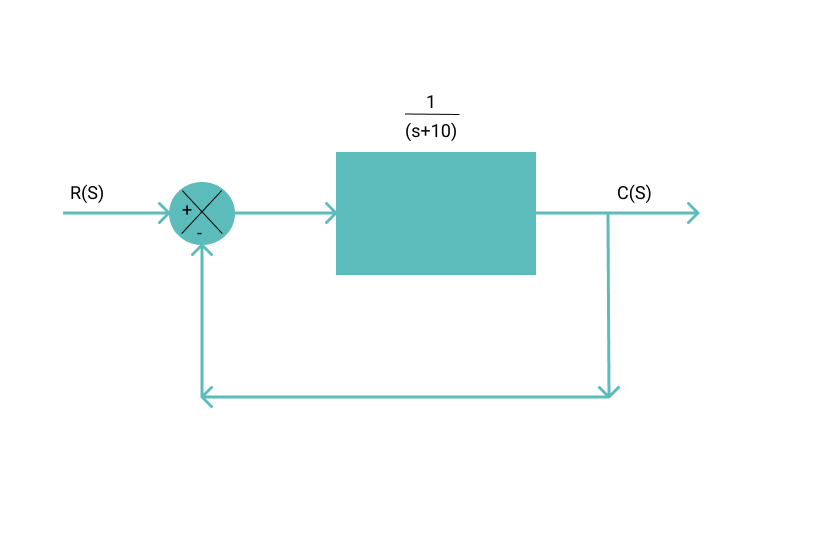
\includegraphics[width =10cm, height = 7cm]{images/exp1.png}
        \caption{Block Diagram}
        \label{Graph}
\end{figure}

\newline

\section*{\textcolor{black}{Theory :}}
Steady-state error is defined as the difference between the desired value and the actual value of a system output in the limit as time goes to infinity (i.e. when the response of the control system has reached steady-state).\par

Steady-state error is a property of the input/output response for a linear system. In general, a good control system will be one that has a low steady-state error
For a Type 0 system, the error is a non-zero, finite number, and Kp is equal to the Bode gain Kx. \par

\section*{\textcolor{black}{Code :}}

   s=\%s;\\ 
   g=syslin('c',1/(s+10))\\
   h=syslin('c',1/(0*s+1))\\
   G= g/.h\\
   t= 0:0.01:5;\\
   y= csim(t,t,G);\\
   plot(t,y)\\
   disp('STEADY STATE ERROR Ess:')\\
   disp(max(t)-max(y)) \par 

\section*{\textcolor{black}{OUTPUT/OBSERVATIONS}}

\begin{figure}[!hth]
        \centering
        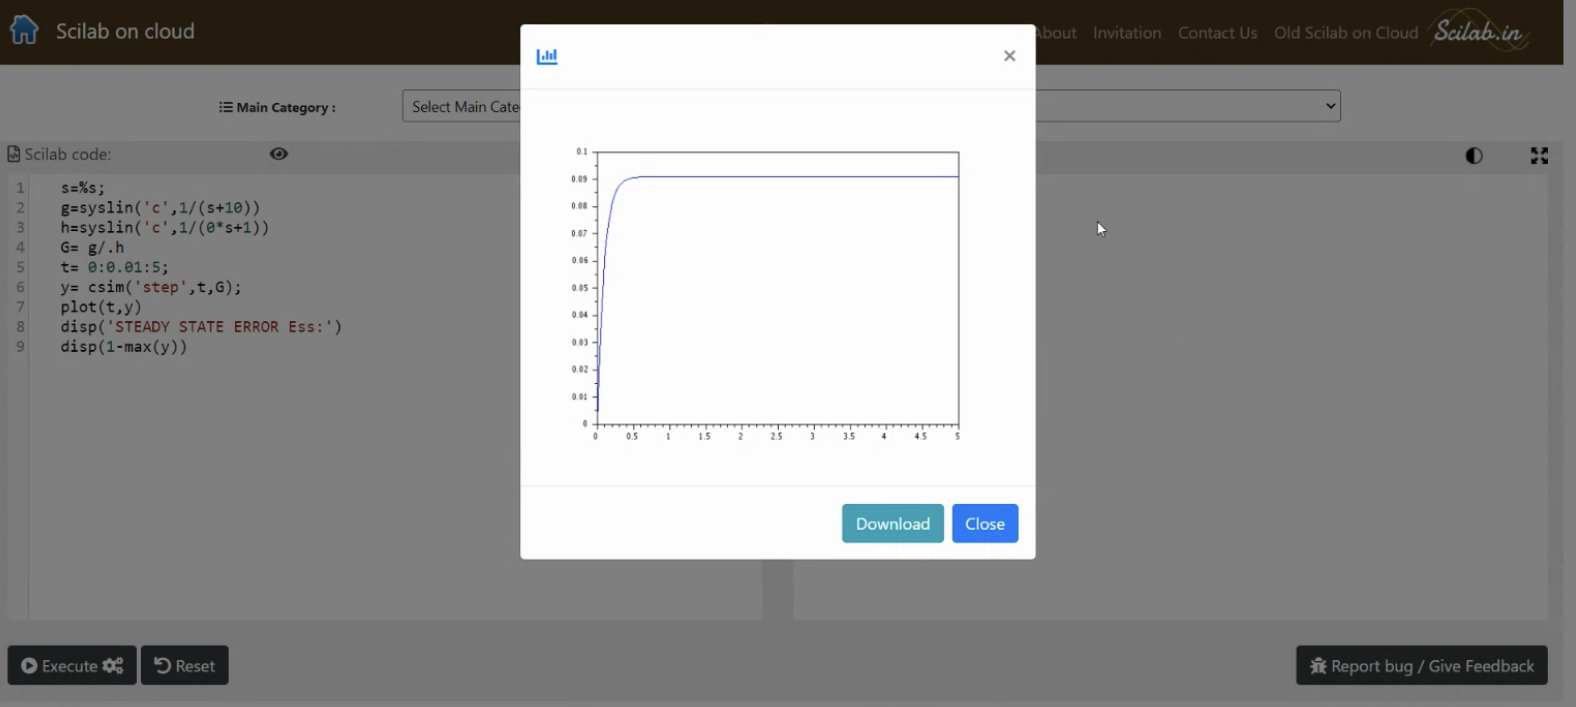
\includegraphics[width =10cm, height = 7cm]{images/exp11.png}
        \caption{Graph}
        \label{Graph}
\end{figure}
\begin{figure}[!hth]
        \centering
        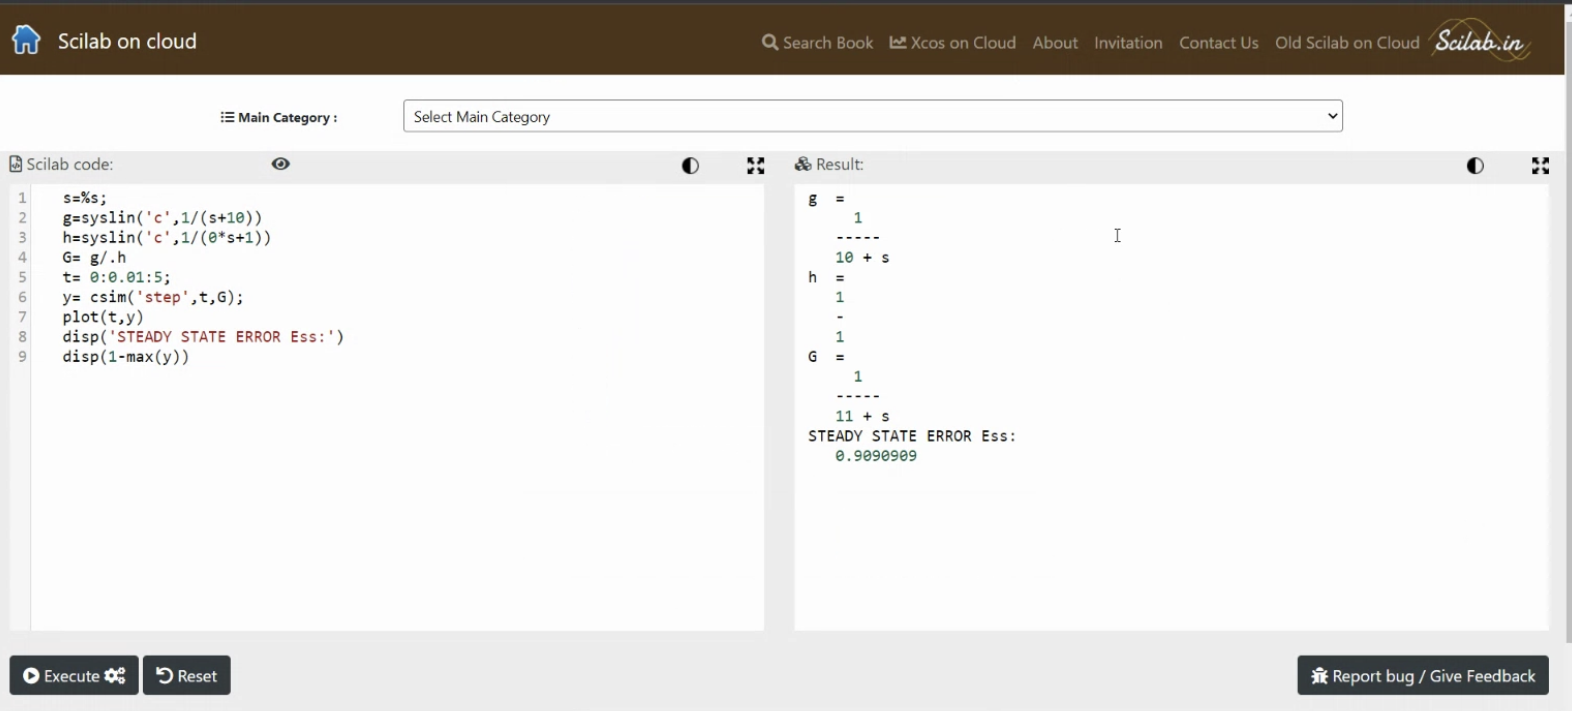
\includegraphics[width =10cm, height = 7cm]{images/exp12.png}
        \caption{Result}
        \label{Result}
\end{figure}

\section*{\textcolor{black}{Conclusion}}
We get a constant error of 0.909 in our case when we give step input in type 0.
 \pagebreak
 
%===============================
%.  Experiment 2
%===============================
\begin{center}
    \LARGE {EXPERIMENT NO : 2}
             
\end{center}

\section*{\textcolor{black}{AIM: }}
\text{To calculate steady state error in position of Type 0}

\section*{\textcolor{black}{Block Diagram :}}
\begin{figure}[!hth]
        \centering
        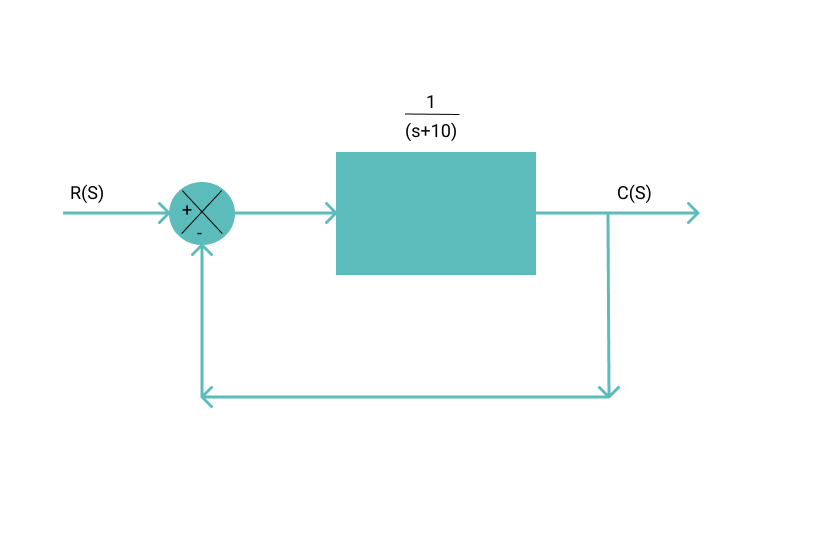
\includegraphics[width =10cm, height = 7cm]{images/exp2.png}
        \caption{Block Diagram}
        \label{Graph}
\end{figure}

\section*{\textcolor{black}{Theory :}}
Steady-state error is defined as the difference between the desired value and the actual value of a system output in the limit as time goes to infinity (i.e. when the response of the control system has reached steady-state).\par

Steady-state error is a property of the input/output response for a linear system. In general, a good control system will be one that has a low steady-state error
For a Type 0 system, the error is a non-zero, finite number, and Kp is equal to the Bode gain Kx. \par

\section*{\textcolor{black}{Code :}}

   s=\%s;\\ 
   g=syslin('c',1/(s+10))\\
   h=syslin('c',1/(0*s+1))\\
   G= g/.h\\
   t= 0:0.01:5;\\
   y= csim('step',t,G);\\
   plot(t,y)\\
   disp('STEADY STATE ERROR Ess:')\\
   disp(1-max(y)) \par 

\section*{\textcolor{black}{OUTPUT/OBSERVATIONS}}

\begin{figure}[!hth]
        \centering
        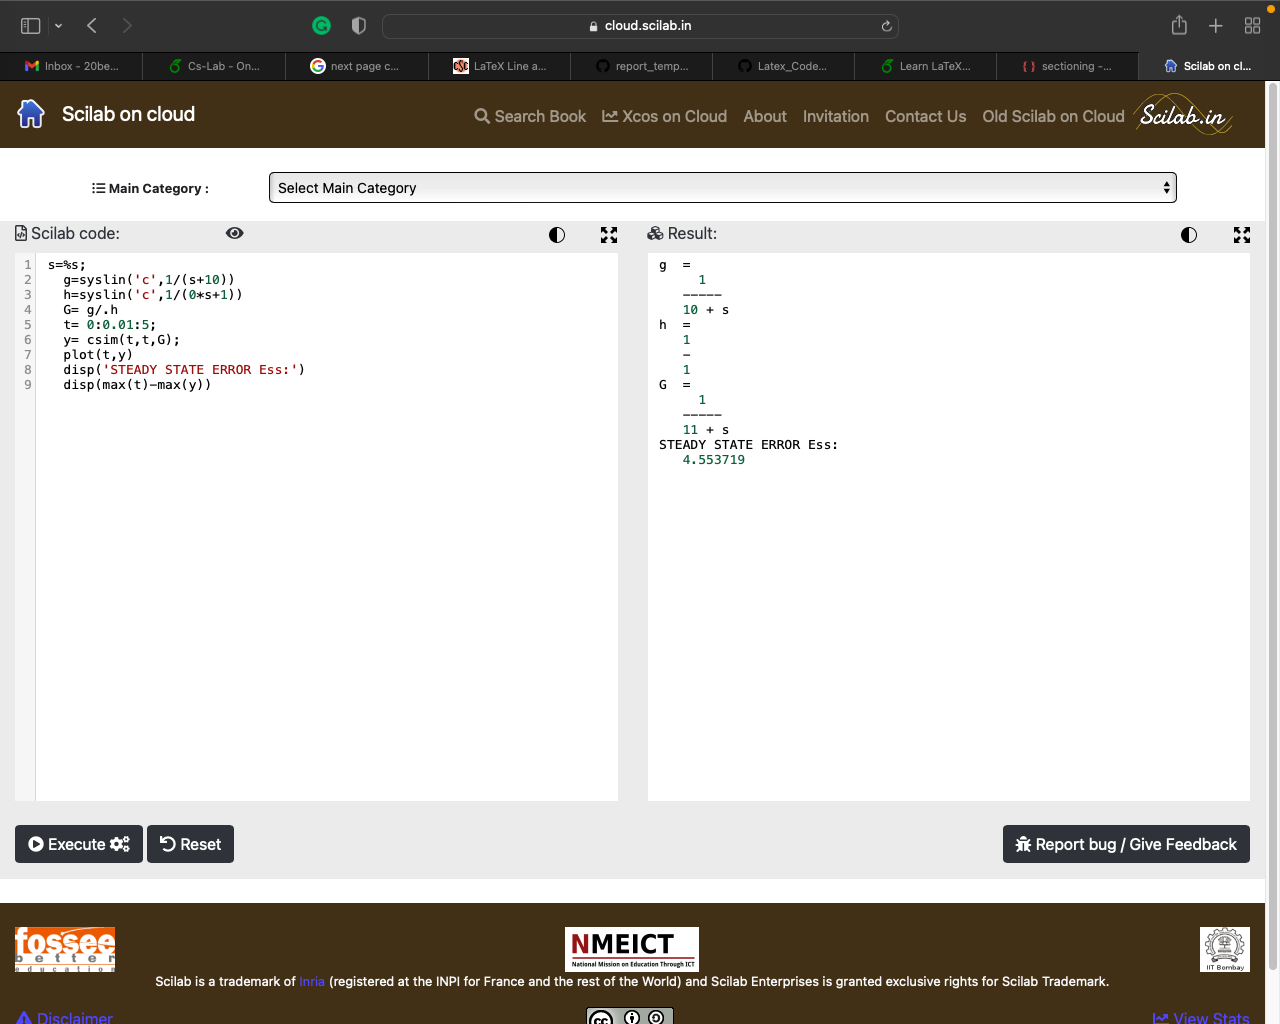
\includegraphics[width =10cm, height = 7cm]{images/exp21.png}
        \caption{Graph}
        \label{Graph}
\end{figure}
\begin{figure}[!hth]
        \centering
        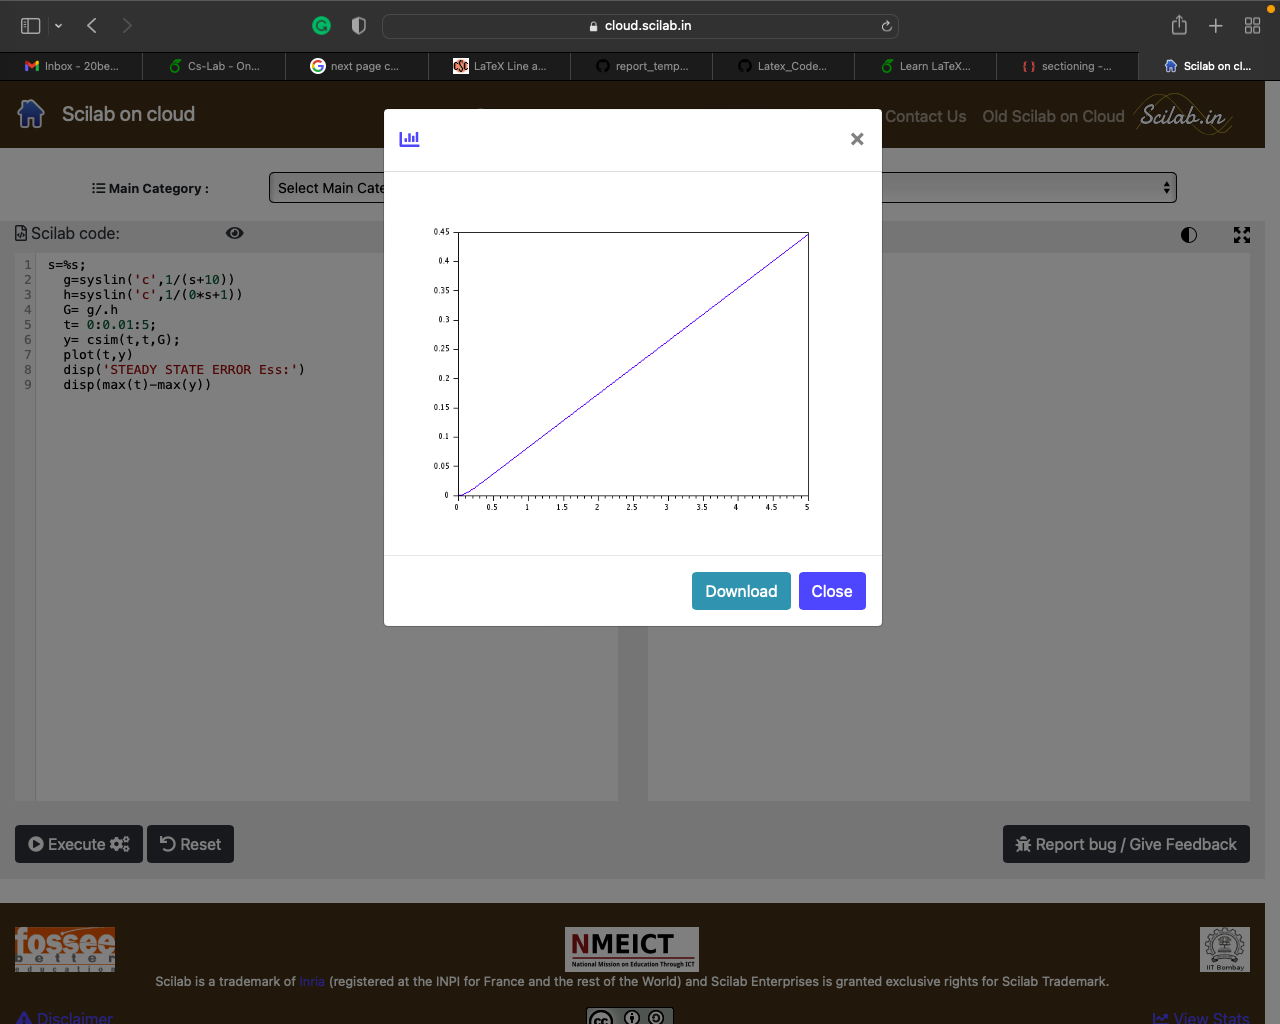
\includegraphics[width =10cm, height = 7cm]{images/exp22.png}
        \caption{Result}
        \label{Result}
\end{figure}

\section*{\textcolor{black}{Conclusion}}
We get a straigth line passing from origin when we give ramp input in type
0 and as we keep on increasing time we get infinte value difference.
\pagebreak
 
 
 
 %===============================
%.  Experiment 3
%===============================
\begin{center}
    \LARGE {EXPERIMENT NO : 3}
             
\end{center}

\section*{\textcolor{black}{AIM: }}
\text{To calculate steady state error in position of Type 0}

\section*{\textcolor{black}{Block Diagram :}}
\begin{figure}[!hth]
        \centering
        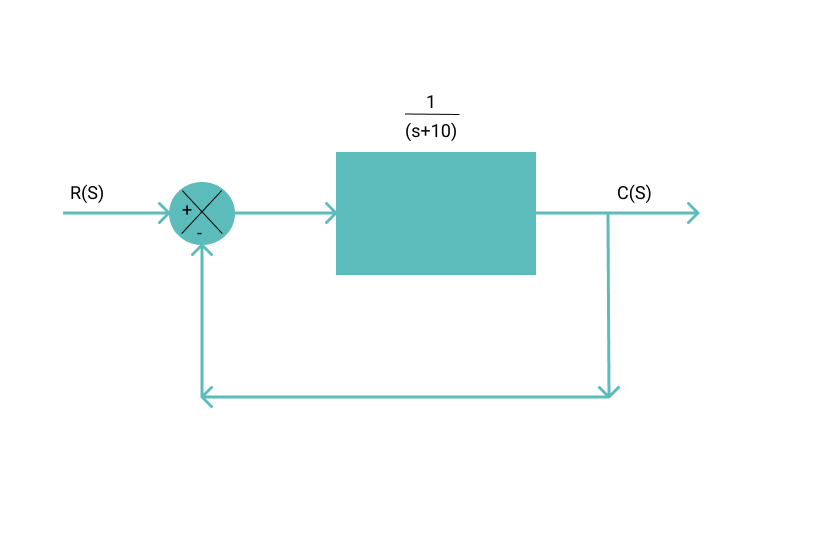
\includegraphics[width =10cm, height = 7cm]{images/exp3.png}
        \caption{Block Diagram}
        \label{Graph}
\end{figure}
\section*{\textcolor{black}{Theory :}}
Steady-state error is defined as the difference between the desired value and the actual value of a system output in the limit as time goes to infinity (i.e. when the response of the control system has reached steady-state).\par

Steady-state error is a property of the input/output response for a linear system. In general, a good control system will be one that has a low steady-state error
For a Type 0 system, the error is a non-zero, finite number, and Kp is equal to the Bode gain Kx. \par

\section*{\textcolor{black}{Code :}}

    s=\%s;\\ 
   g=syslin('c',1/(s+10))\\
   h=syslin('c',1/(0*s+1))\\
   G= g/.h\\
   t= 0:0.01:5;\\
   y= csim(t.\wedge2,t,G);\\
   plot(t,y)\\
   disp('STEADY STATE ERROR Ess:')\\
   disp(max(t.\wedge2)-max(y)) \par 

\section*{\textcolor{black}{OUTPUT/OBSERVATIONS}}

\begin{figure}[!hth]
        \centering
        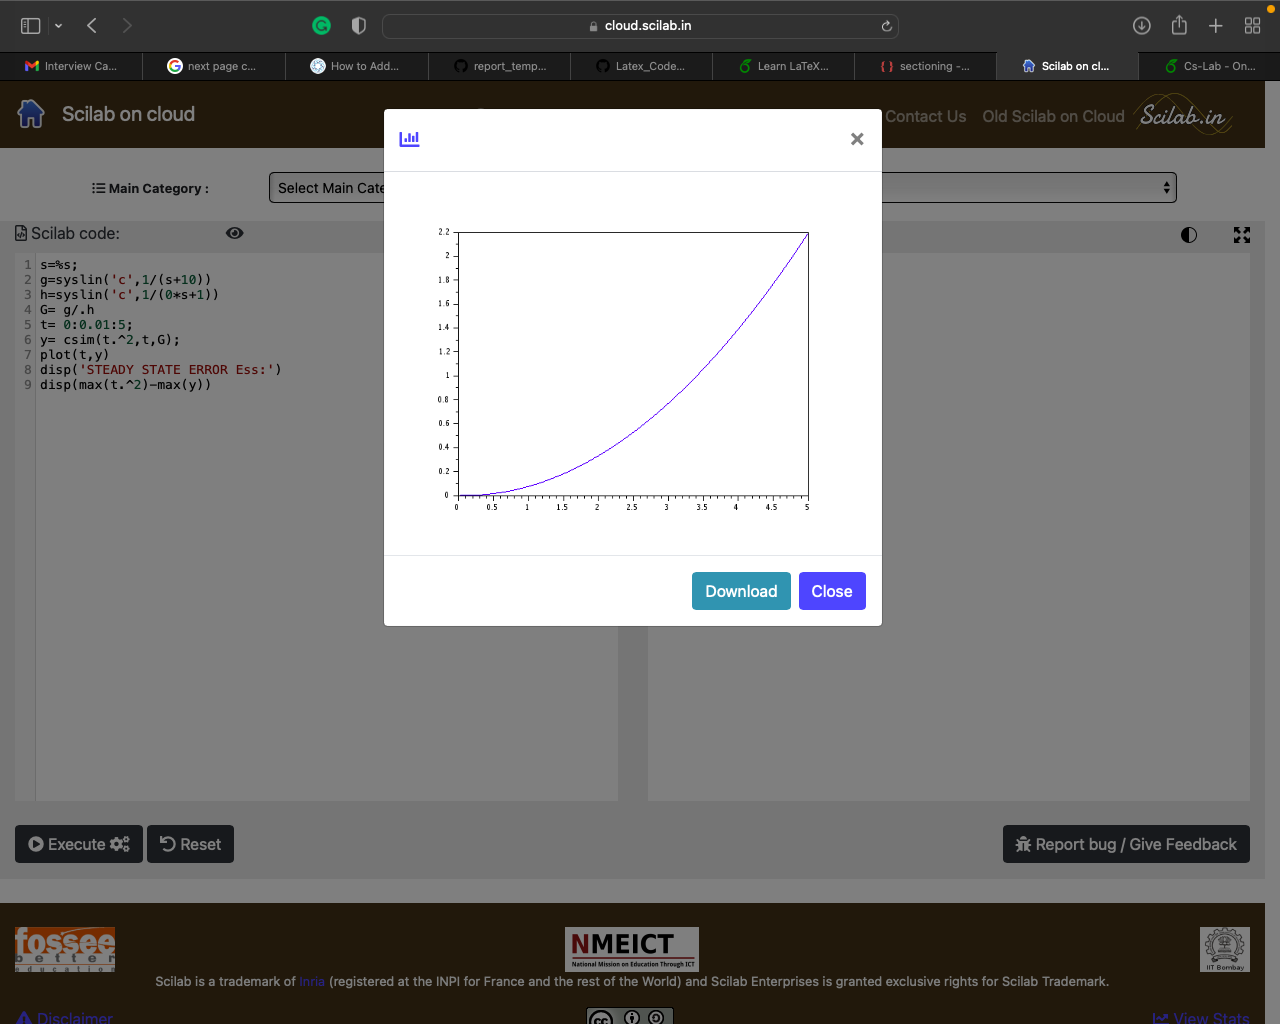
\includegraphics[width =10cm, height = 7cm]{images/exp31.png}
        \caption{Graph}
        \label{Graph}
\end{figure}
\begin{figure}[!hth]
        \centering
        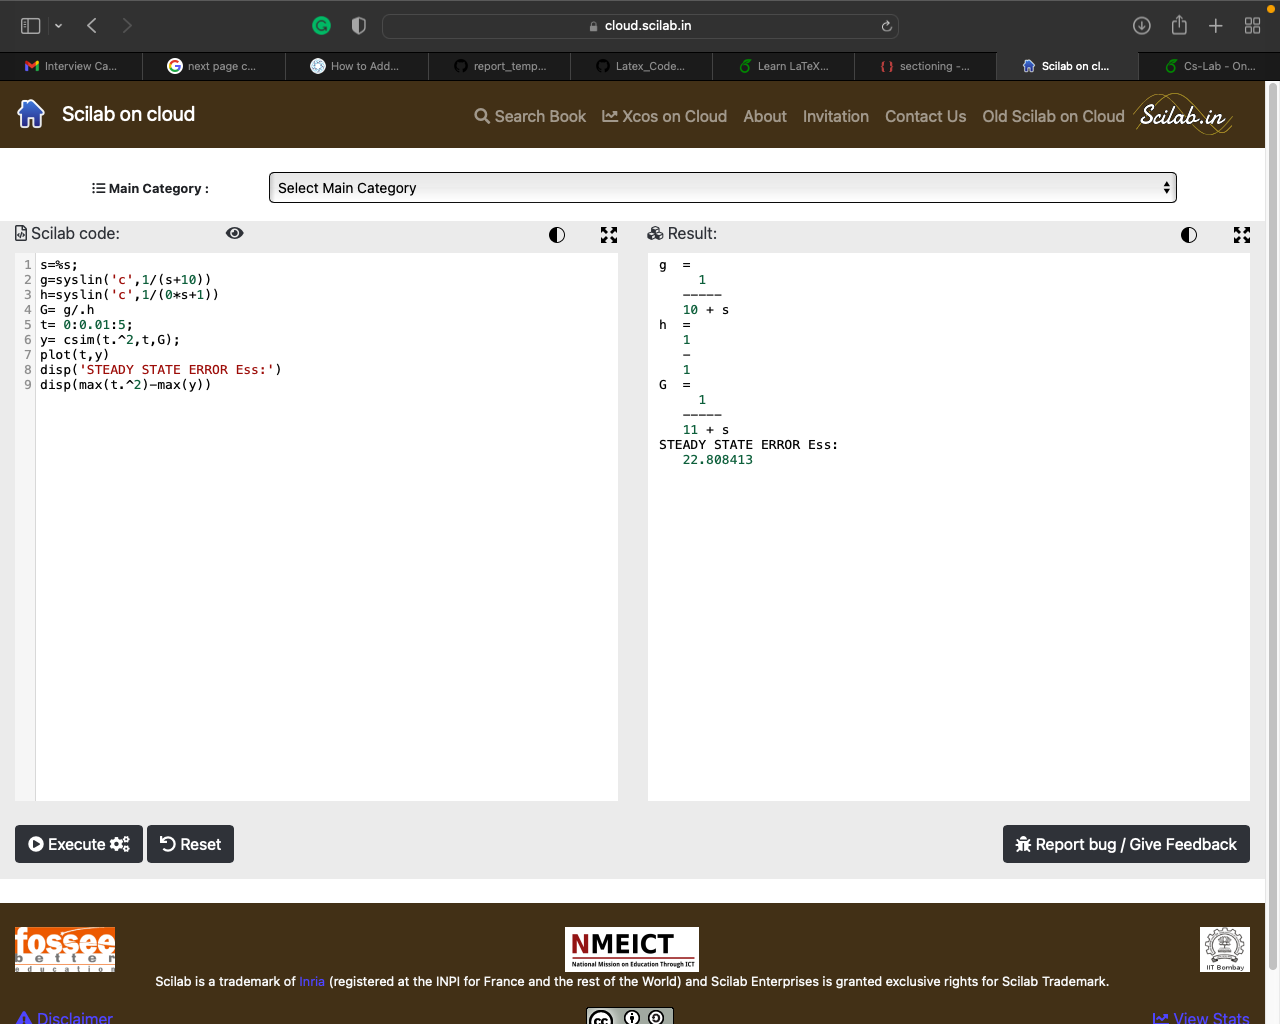
\includegraphics[width =10cm, height = 7cm]{images/exp32.png}
        \caption{Result}
        \label{Result}
\end{figure}

\section*{\textcolor{black}{Conclusion}}
 We get a parabolic curve when we give parabolic input in type 0 and as we keep on increasing time we get infinte value difference
 \pagebreak
 
 \begin{center}
    \LARGE {EXPERIMENT NO : 4}
             
\end{center}

\section*{\textcolor{black}{AIM: }}
\text{To calculate steady state error in position of Type 1}

\section*{\textcolor{black}{Block Diagram :}}
 \begin{figure}[!hth]
        \centering
        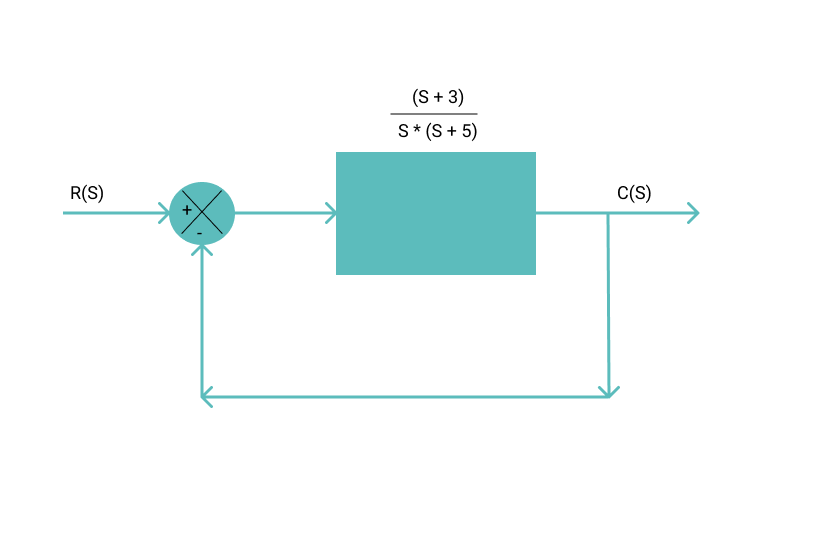
\includegraphics[width =10cm, height = 7cm]{images/exp4.png}
        \caption{Block Diagram}
        \label{Graph}
\end{figure}

\section*{\textcolor{black}{Theory :}}
Steady-state error is defined as the difference between the desired value and the actual value of a system output in the limit as time goes to infinity (i.e. when the response of the control system has reached steady-state).\par

Steady-state error is a property of the input/output response for a linear system. In general, a good control system will be one that has a low steady-state error
For a Type 0 system, the error is a non-zero, finite number, and Kp is equal to the Bode gain Kx. \par

\section*{\textcolor{black}{Code :}}

   s=\%s;\\ 
   g=syslin('c',(s+3)/s*(s+5))\\
   h=syslin('c',1/(0*s+1))\\
   G= g/.h\\
   t= 0:0.01:5;\\
   y= csim('step',t,G);\\
   plot(t,y)\\
   disp('STEADY STATE ERROR Ess:')\\
   disp(1-max(y)) \par 

\section*{\textcolor{black}{OUTPUT/OBSERVATIONS}}


\begin{figure}[!hth]
        \centering
        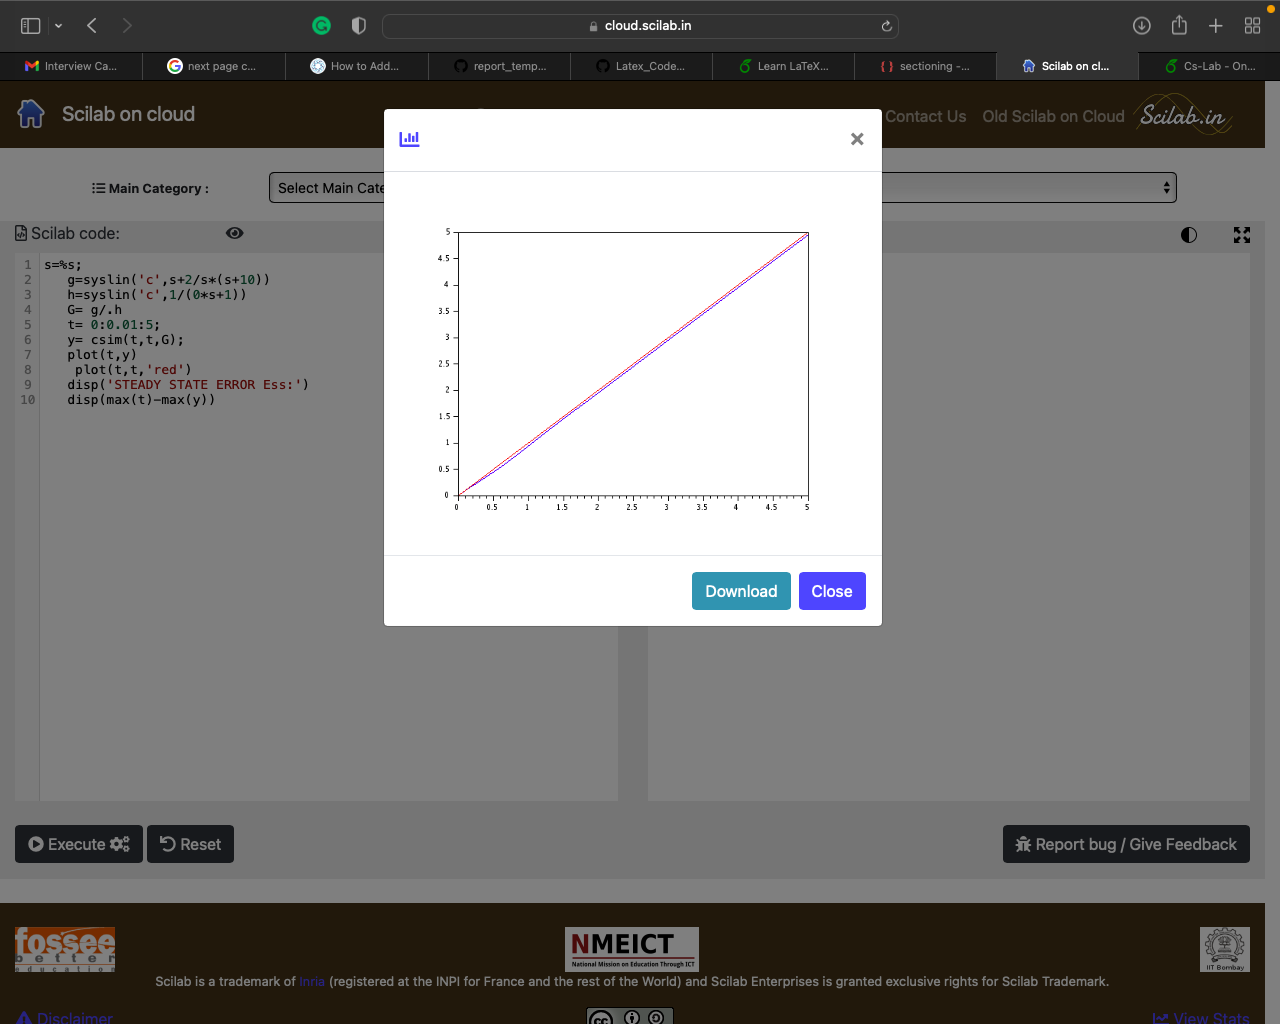
\includegraphics[width =10cm, height = 10cm]{images/exp41.png}
        \caption{Graph}
        \label{Result}
        
\end{figure}
        \begin{figure}[!hth]
        \centering
        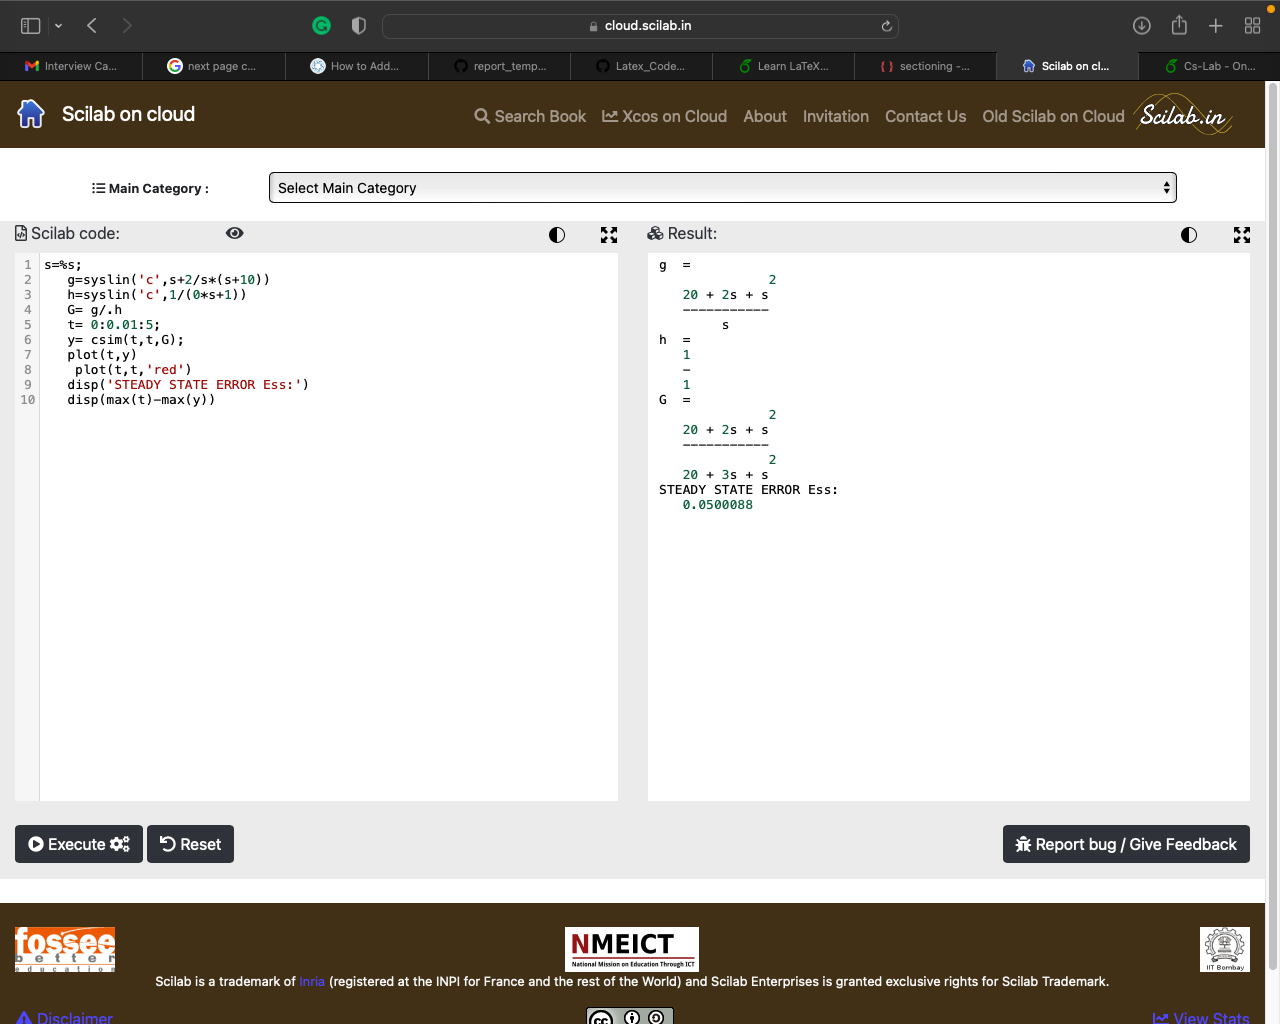
\includegraphics[width =10cm, height = 10cm]{images/exp42.png}
        \caption{Result}
        \label{Result}
\end{figure}

\section*{\textcolor{black}{Conclusion}}
We get a constant graph and as we increase the time , the error becomes 0 in case of step input in type 1.
  \pagebreak

\begin{center}
    \LARGE {EXPERIMENT NO : 5}
             
\end{center}

\section*{\textcolor{black}{AIM: }}
\text{To calculate steady state error in position of Type 1}

\section*{\textcolor{black}{Block Diagram :}}
\begin{figure}[!hth]
        \centering
        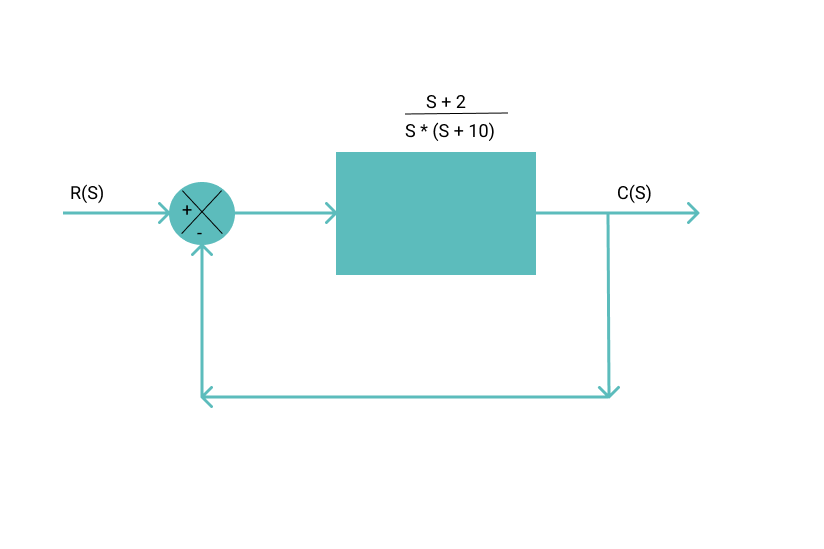
\includegraphics[width =10cm, height = 7cm]{images/exp5.png}
        \caption{Block Diagram}
        \label{Graph}
\end{figure}
\section*{\textcolor{black}{Theory :}}
Steady-state error is defined as the difference between the desired value and the actual value of a system output in the limit as time goes to infinity (i.e. when the response of the control system has reached steady-state).\par

Steady-state error is a property of the input/output response for a linear system. In general, a good control system will be one that has a low steady-state error
For a Type 0 system, the error is a non-zero, finite number, and Kp is equal to the Bode gain Kx. \par

\section*{\textcolor{black}{Code :}}

   s=\%s;\\ 
   g=syslin('c',s+2/s*(s+10))\\
   h=syslin('c',1/(0*s+1))\\
   G= g/.h\\
   t= 0:0.01:5;\\
   y= csim(t,t,G);\\
   plot(t,y)\\
    plot(t,t,'red')\\
   disp('STEADY STATE ERROR Ess:')\\
   disp(max(t)-max(y)) \par 

\section*{\textcolor{black}{OUTPUT/OBSERVATIONS}}

\begin{figure}[!hth]
        \centering
        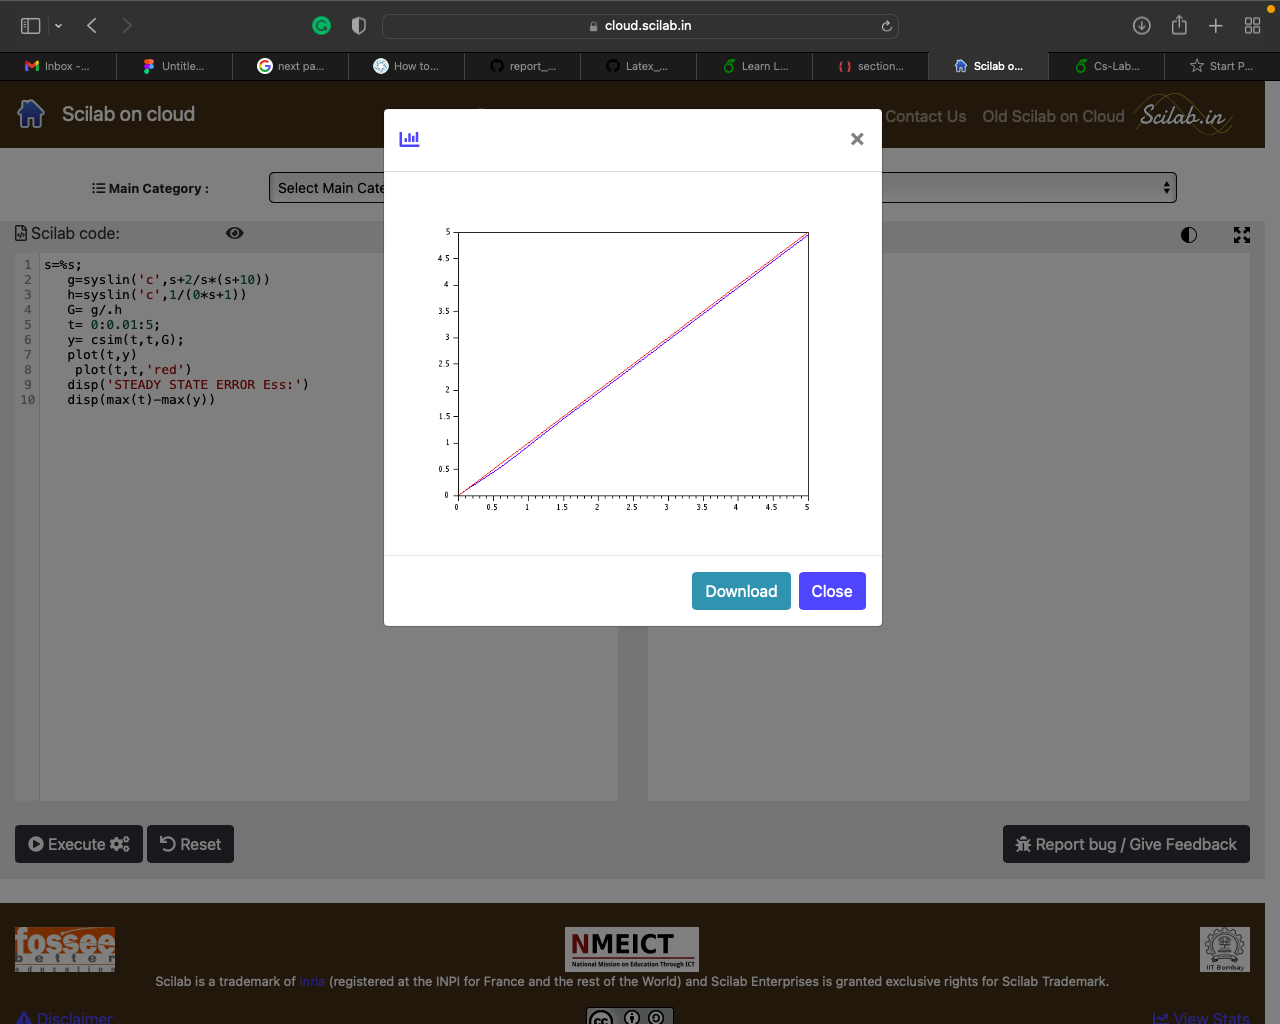
\includegraphics[width =10cm, height = 10cm]{images/exp51.png}
        \caption{Graph}
        \label{Graph}
\end{figure}
\begin{figure}[!hth]
        \centering
        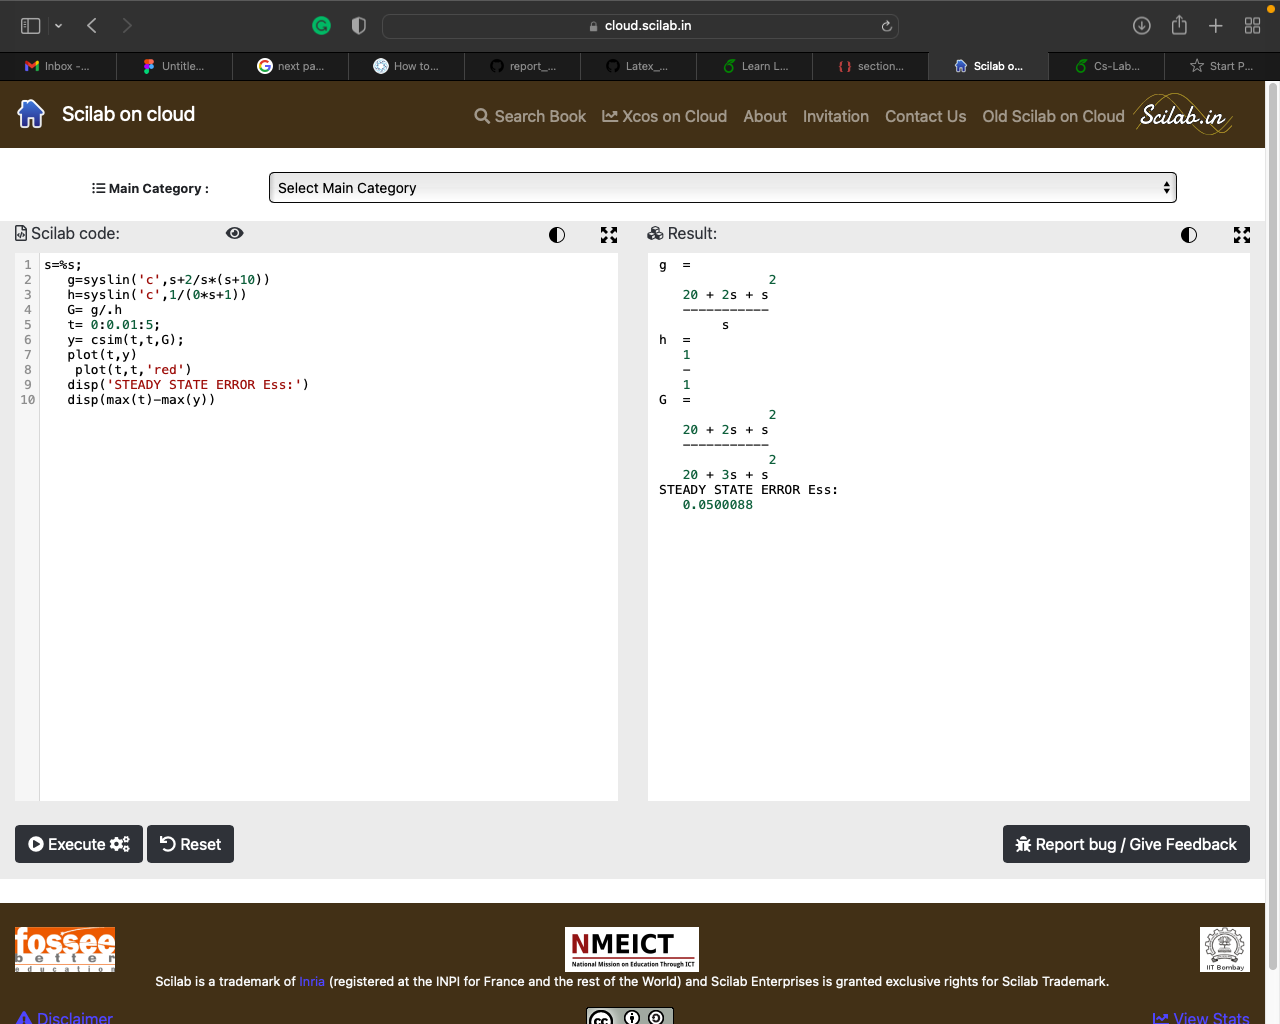
\includegraphics[width =10cm, height = 10cm]{images/exp52.png}
        \caption{Result}
        \label{Result}
\end{figure}

\section*{\textcolor{black}{Conclusion}}
We get a constant difference i.e. constant error which is equal to 1/Kv when we use ramp input in type 1.
 \pagebreak
 
 \begin{center}
    \LARGE {EXPERIMENT NO : 6}
             
\end{center}

\section*{\textcolor{black}{AIM: }}
\text{To calculate steady state error in acceleration of Type 1}

\section*{\textcolor{black}{Block Diagram :}}

\begin{figure}[!hth]
        \centering
        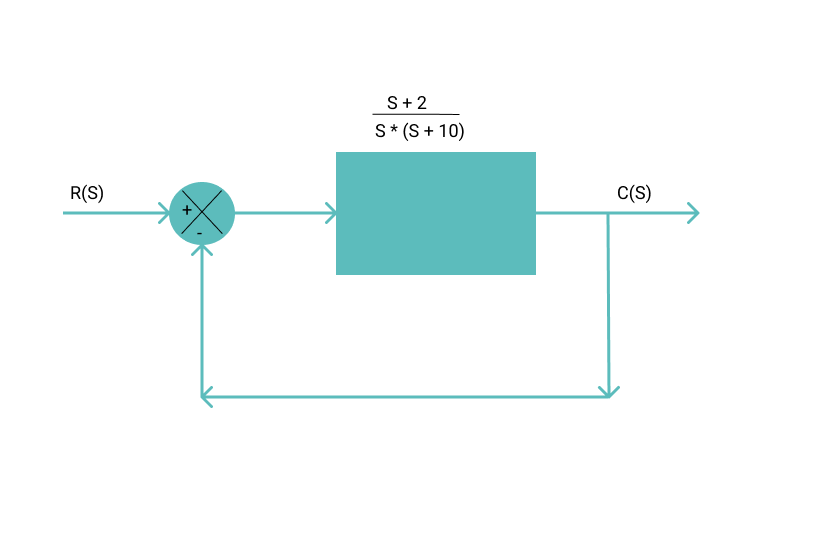
\includegraphics[width =10cm, height = 7cm]{images/exp6.png}
        \caption{Block Diagram}
        \label{Graph}
\end{figure}

\section*{\textcolor{black}{Theory :}}
Steady-state error is defined as the difference between the desired value and the actual value of a system output in the limit as time goes to infinity (i.e. when the response of the control system has reached steady-state).\par

Steady-state error is a property of the input/output response for a linear system. In general, a good control system will be one that has a low steady-state error
For a Type 0 system, the error is a non-zero, finite number, and Kp is equal to the Bode gain Kx. \par

\section*{\textcolor{black}{Code :}}

   s=\%s;\\ 
   g=syslin('c',(s+2)/s*(s+10))\\
   h=syslin('c',1/(0*s+1))\\
   G= g/.h\\
   t= 0:0.01:5;\\
   y= csim(t.\wedge2,t,G);\\
   plot(t,y)\\
    plot(t,t.\wedge2,'red')\\
   disp('STEADY STATE ERROR Ess:')\\
   disp(max(t.\wedge2)-max(y)) \par 

\section*{\textcolor{black}{OUTPUT/OBSERVATIONS}}

\begin{figure}[!hth]
        \centering
        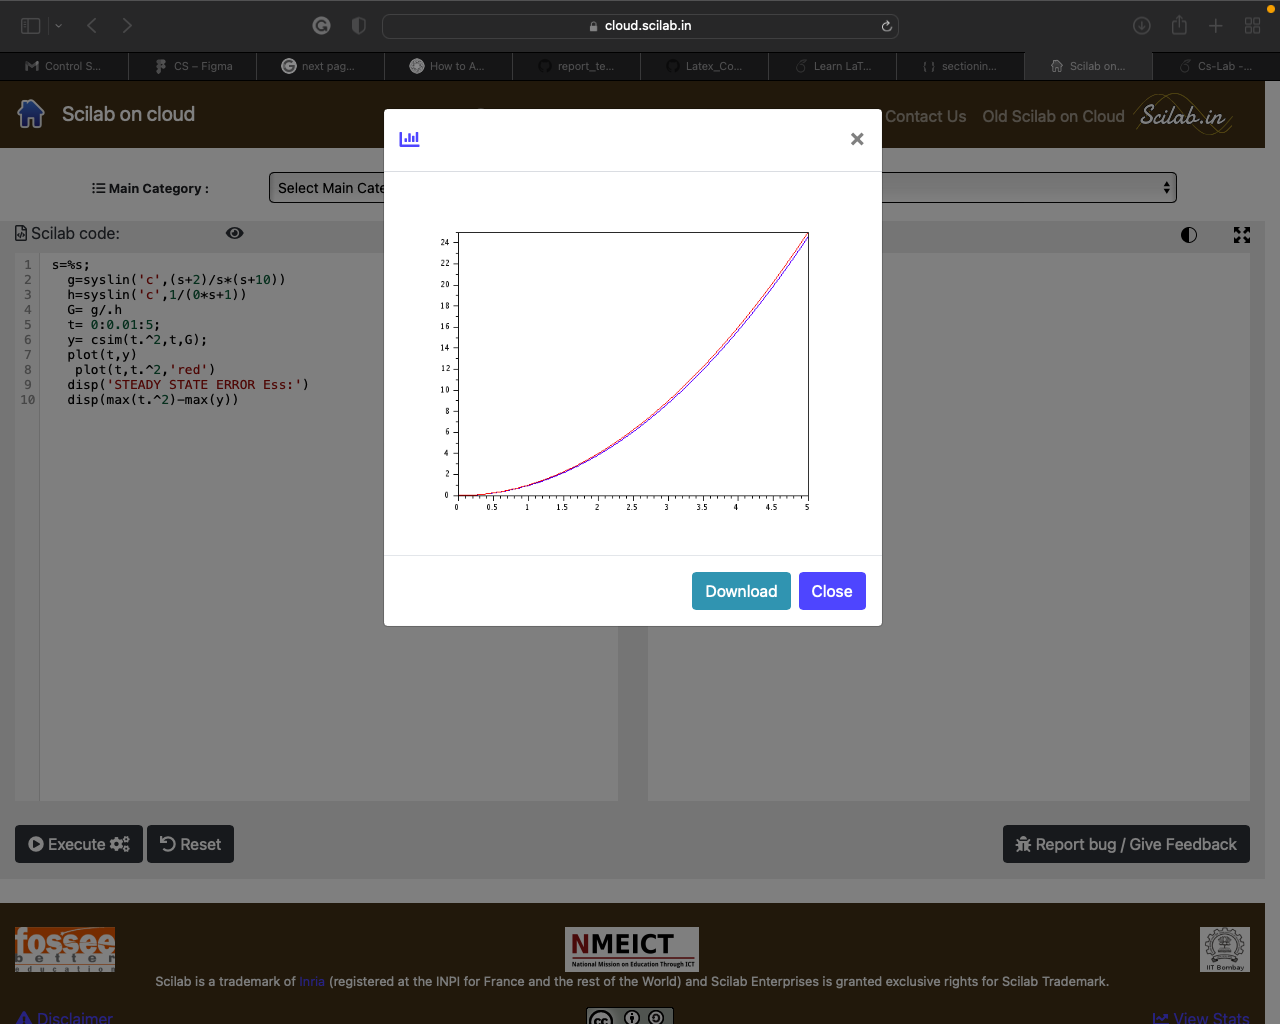
\includegraphics[width =10cm, height = 10cm]{images/exp61.png}
        \caption{Graph}
        \label{Graph}
\end{figure}
\begin{figure}[!hth]
        \centering
        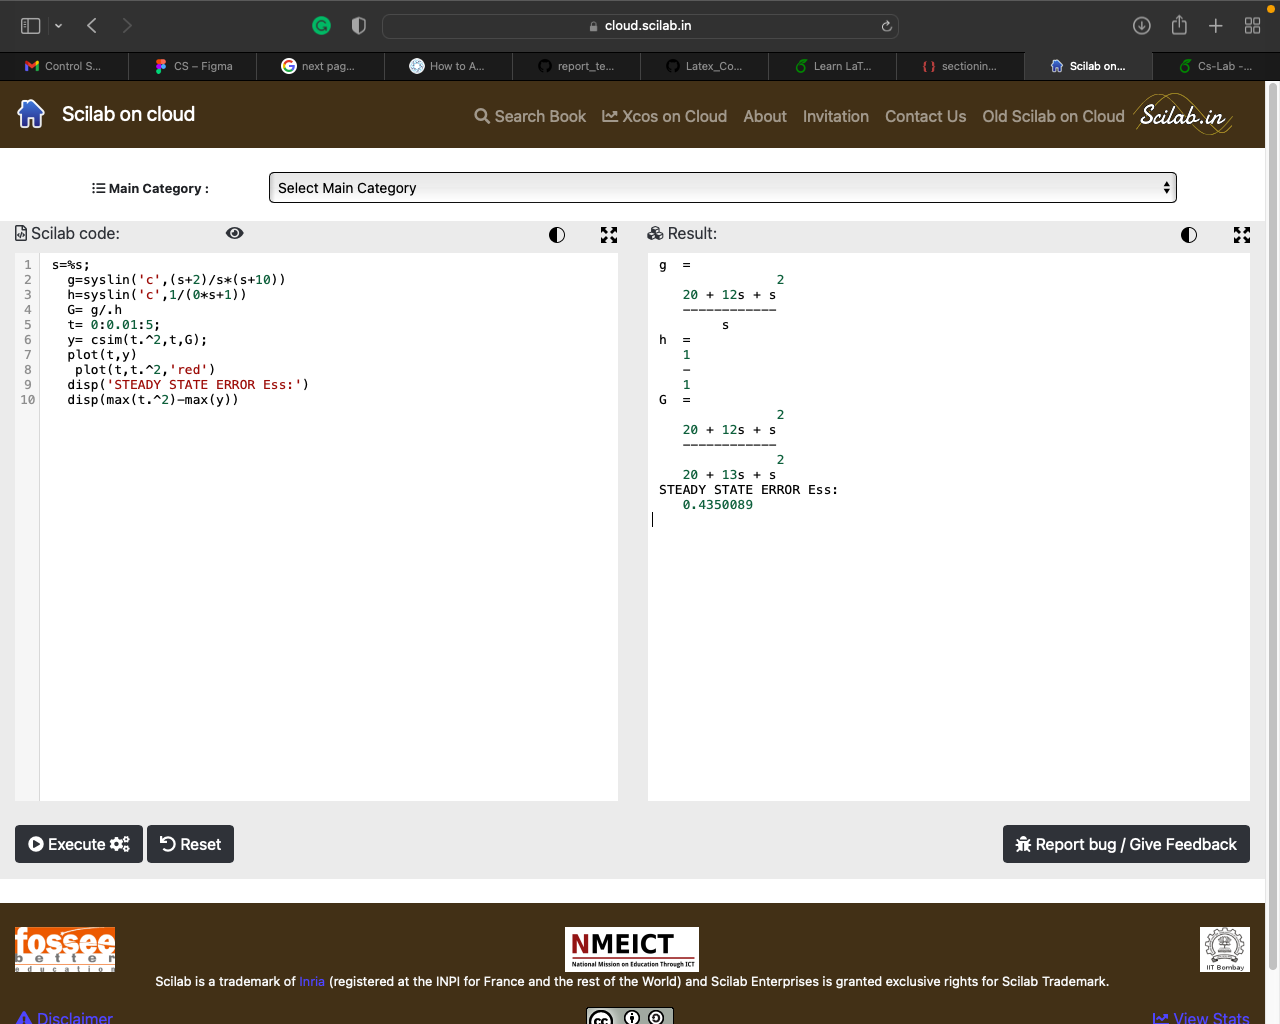
\includegraphics[width =10cm, height = 10cm]{images/exp62.png}
        \caption{Result}
        \label{Result}
\end{figure}


\section*{\textcolor{black}{Conclusion}}
 When we use a parabolic input in type 1 we get an increasing error which becomes infinite as we increase the time to infinite.
   \pagebreak
\maketitle
\begin{center}
    \LARGE {EXPERIMENT NO : 7}
             
\end{center}

\section*{\textcolor{black}{AIM: }}
\text{To calculate steady state error in position of Type 2}

\section*{\textcolor{black}{Block Diagram :}}

\begin{figure}[!hth]
        \centering
        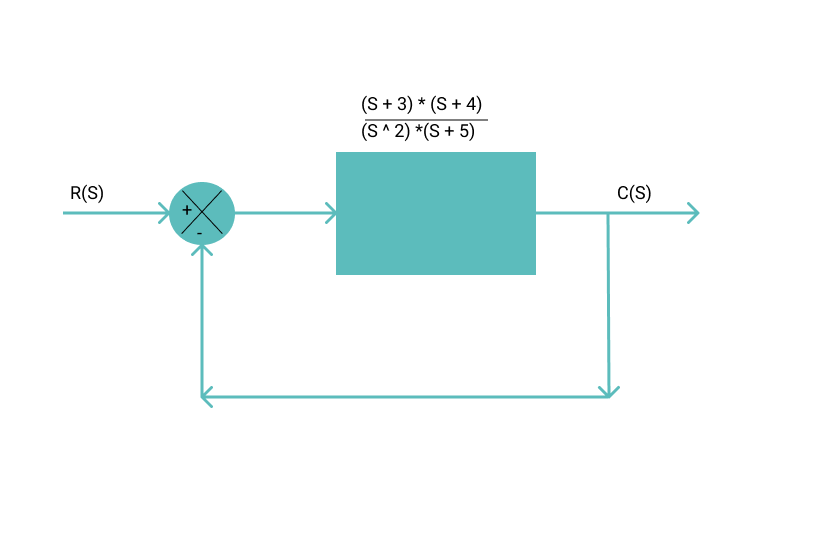
\includegraphics[width =10cm, height = 7cm]{images/exp7.png}
        \caption{Block Diagram}
        \label{Graph}
\end{figure}

\section*{\textcolor{black}{Theory :}}
Steady-state error is defined as the difference between the desired value and the actual value of a system output in the limit as time goes to infinity (i.e. when the response of the control system has reached steady-state).\par

Steady-state error is a property of the input/output response for a linear system. In general, a good control system will be one that has a low steady-state error
For a Type 0 system, the error is a non-zero, finite number, and Kp is equal to the Bode gain Kx. \par

\section*{\textcolor{black}{Code :}}

   s=\%s;\\ 
   g=syslin('c',(s+4)(s+3)/s.\wedge2(s+5))\\
   t= 0:0.01:5;\\
   y= csim('step',t,G);\\
   plot(t,y)\\
    plot(t,t,'red')\\
   disp('STEADY STATE ERROR Ess:')\\
   disp(1-max(y)) \par 

\section*{\textcolor{black}{OUTPUT/OBSERVATIONS}}

\begin{figure}[!hth]
        \centering
        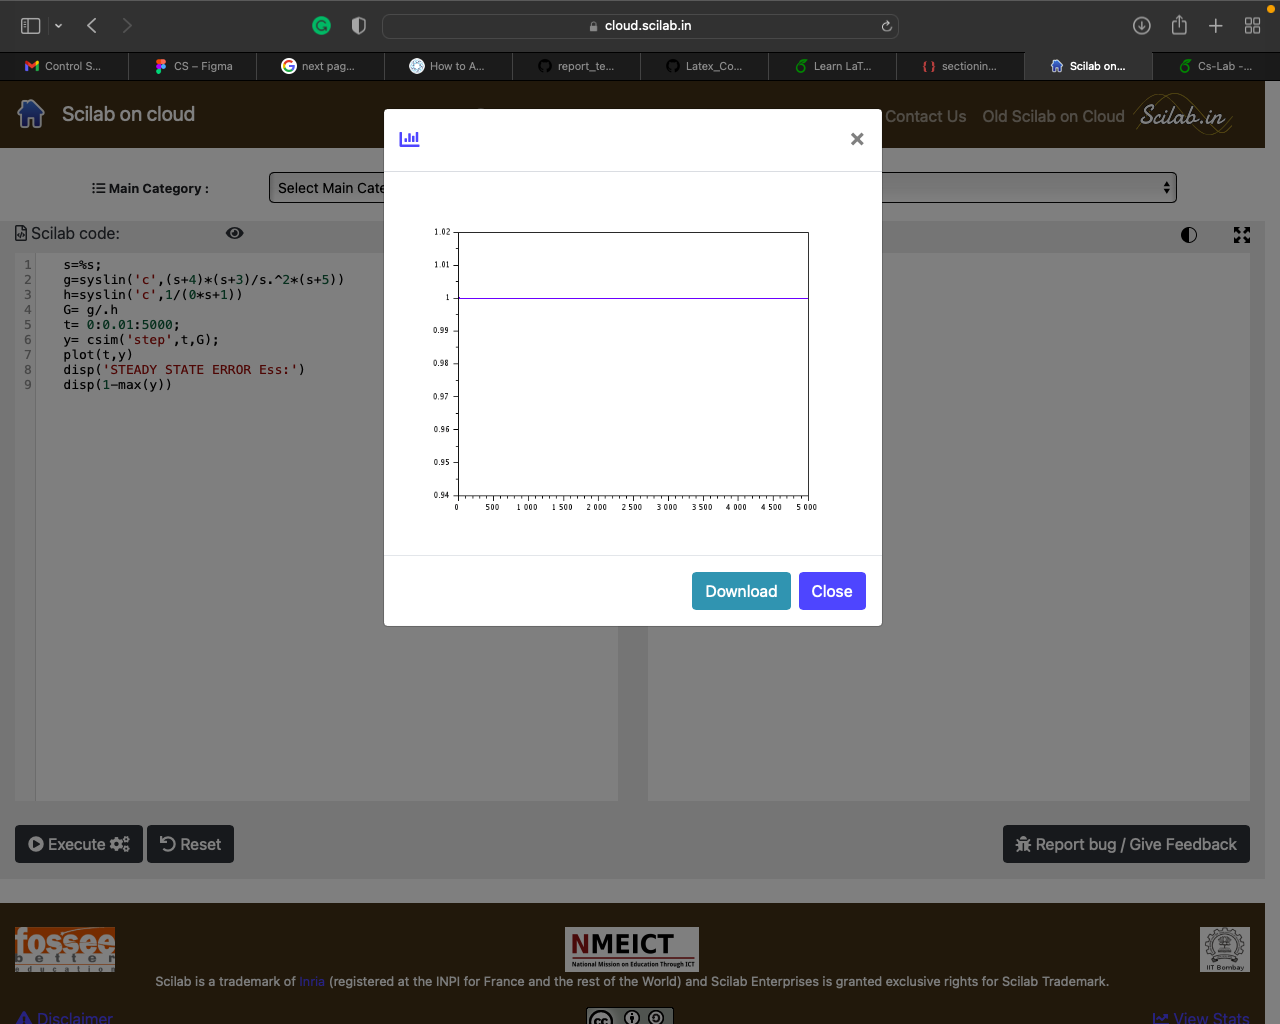
\includegraphics[width =10cm, height = 10cm]{images/exp71.png}
        \caption{Graph}
        \label{Graph}
\end{figure}
\begin{figure}[!hth]
        \centering
        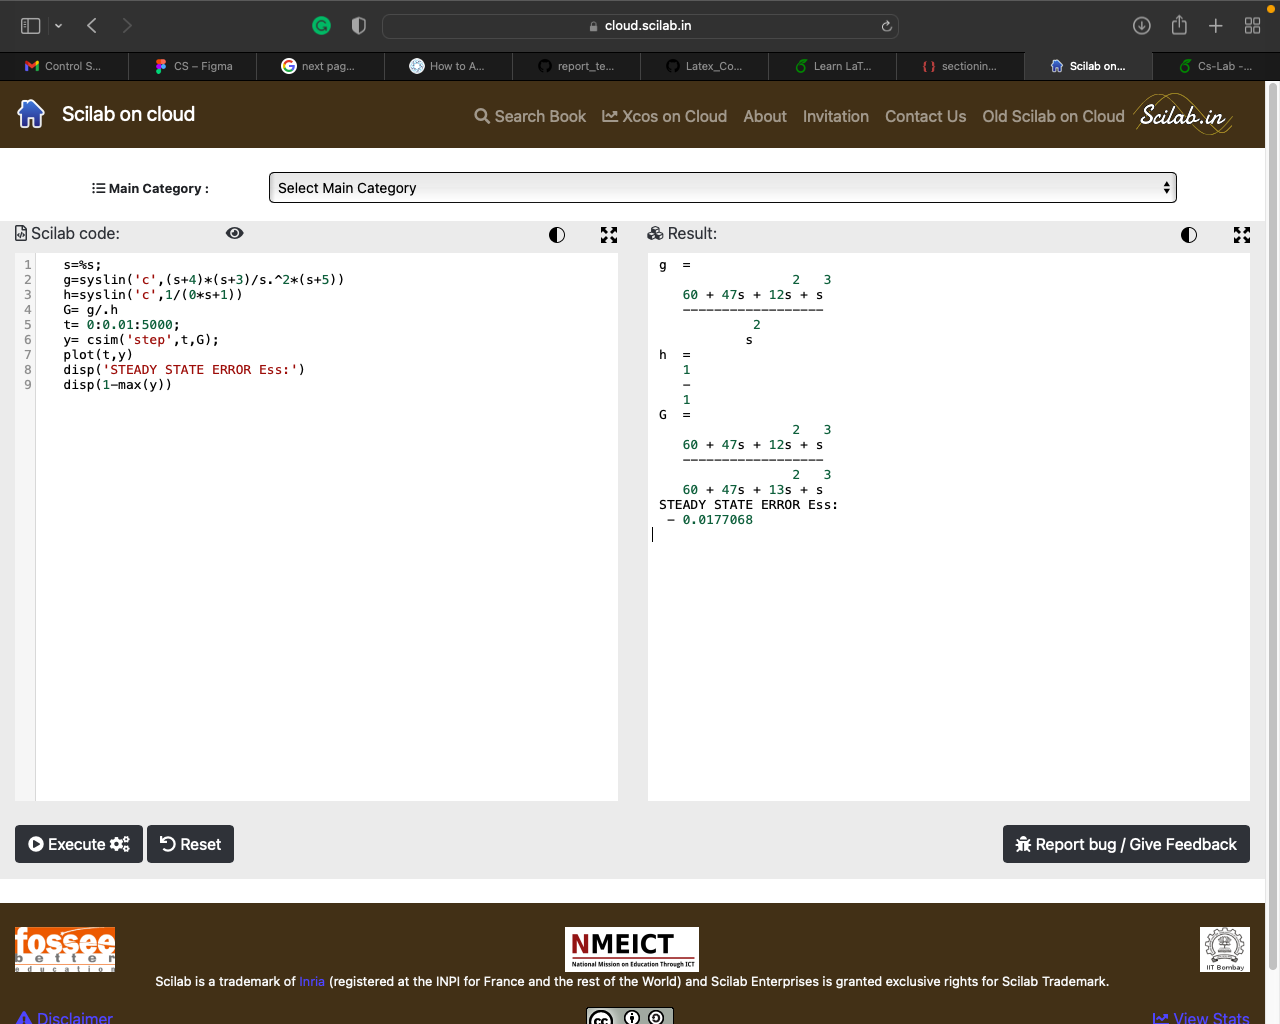
\includegraphics[width =10cm, height = 10cm]{images/exp72.png}
        \caption{Result}
        \label{Result}
\end{figure}

\section*{\textcolor{black}{Conclusion}}
 We get zero difference i.e zero error for step input in type 2 as we increase the time.
    \pagebreak
\maketitle
\begin{center}
    \LARGE {EXPERIMENT NO : 8}
             
\end{center}

\section*{\textcolor{black}{AIM: }}
\text{To calculate steady state error in velocity of Type 2}

\section*{\textcolor{black}{Block Diagram :}}

\begin{figure}[!hth]
        \centering
        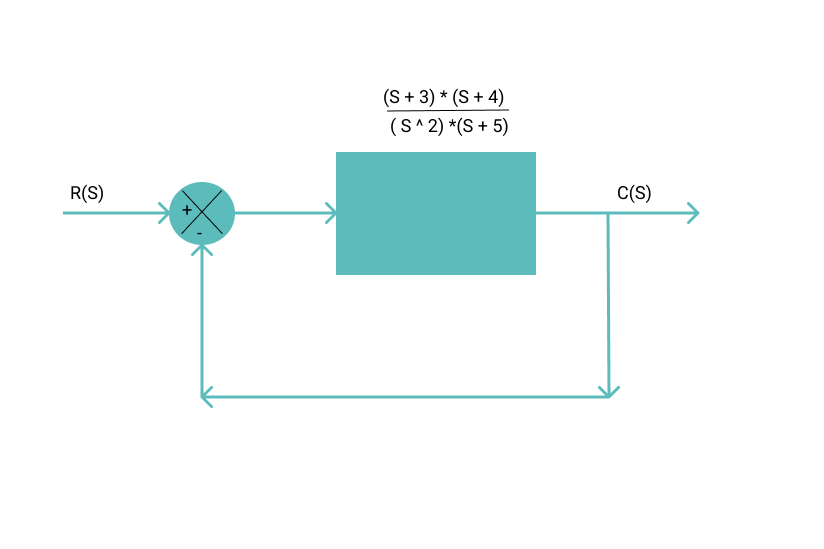
\includegraphics[width =10cm, height = 7cm]{images/exp8.png}
        \caption{Block Diagram}
        \label{Graph}
\end{figure}

\section*{\textcolor{black}{Theory :}}
Steady-state error is defined as the difference between the desired value and the actual value of a system output in the limit as time goes to infinity (i.e. when the response of the control system has reached steady-state).\par

Steady-state error is a property of the input/output response for a linear system. In general, a good control system will be one that has a low steady-state error
For a Type 0 system, the error is a non-zero, finite number, and Kp is equal to the Bode gain Kx. \par

\section*{\textcolor{black}{Code :}}

   s=\%s;\\ 
   g=syslin('c',(s+4)(s+3)/s.\wedge2(s+5))\\
   h=syslin('c',1/(0*s+1))\\
   G= g/.h\\
   t= 0:0.01:5;\\
   y= csim(t,t,G);\\
   plot(t,y)\\
    plot(t,t,'red')\\
   disp('STEADY STATE ERROR Ess:')\\
   disp(max(t)-max(y)) \par 

\section*{\textcolor{black}{OUTPUT/OBSERVATIONS}}

\begin{figure}[!hth]
        \centering
        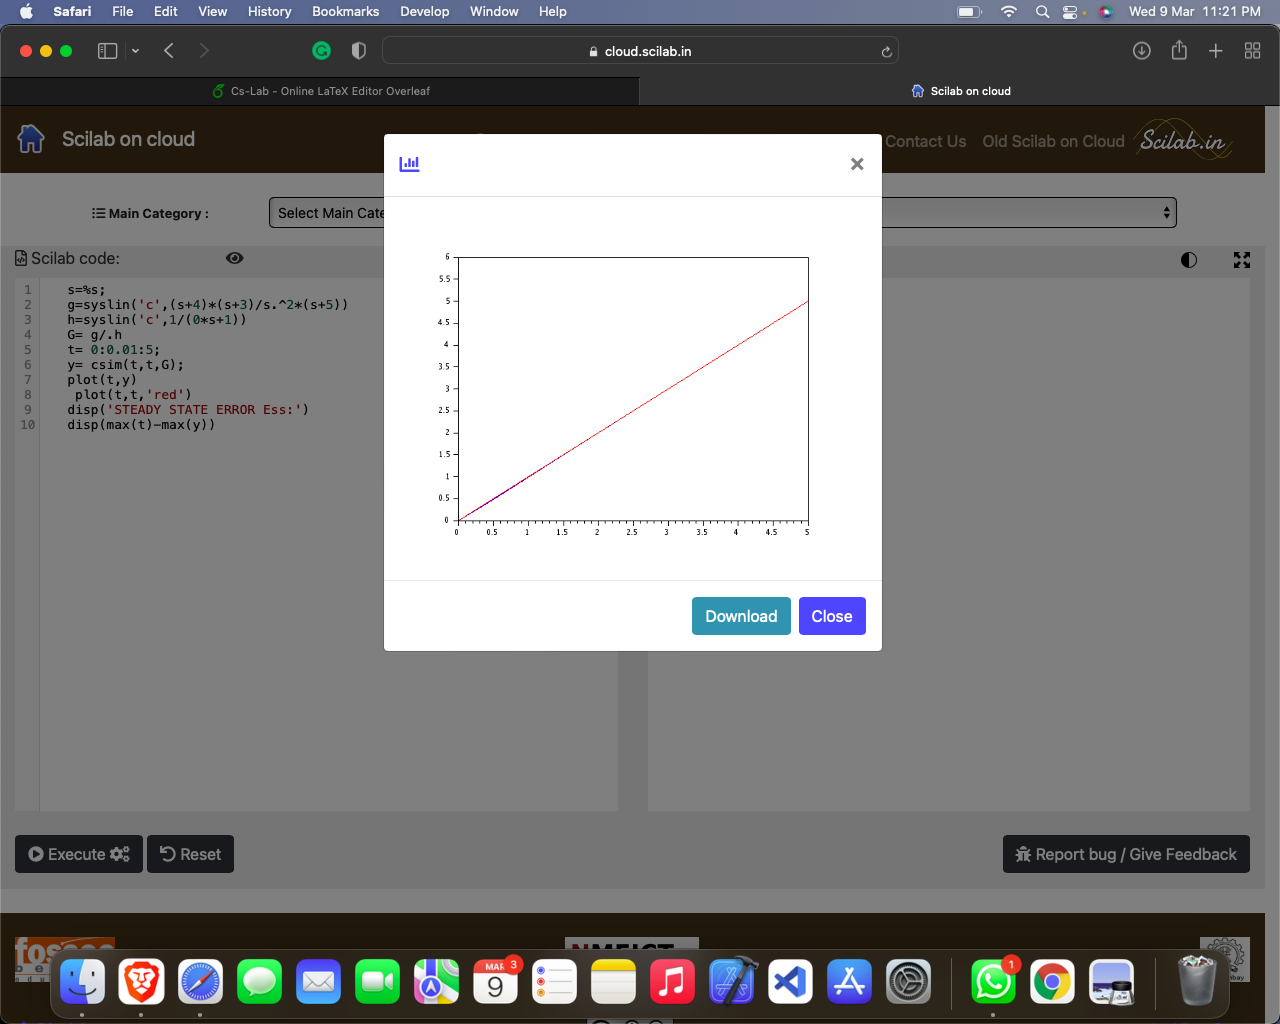
\includegraphics[width =10cm, height = 10cm]{images/exp81.png}
        \caption{Graph}
        \label{Graph}
\end{figure}
\begin{figure}[!hth]
        \centering
        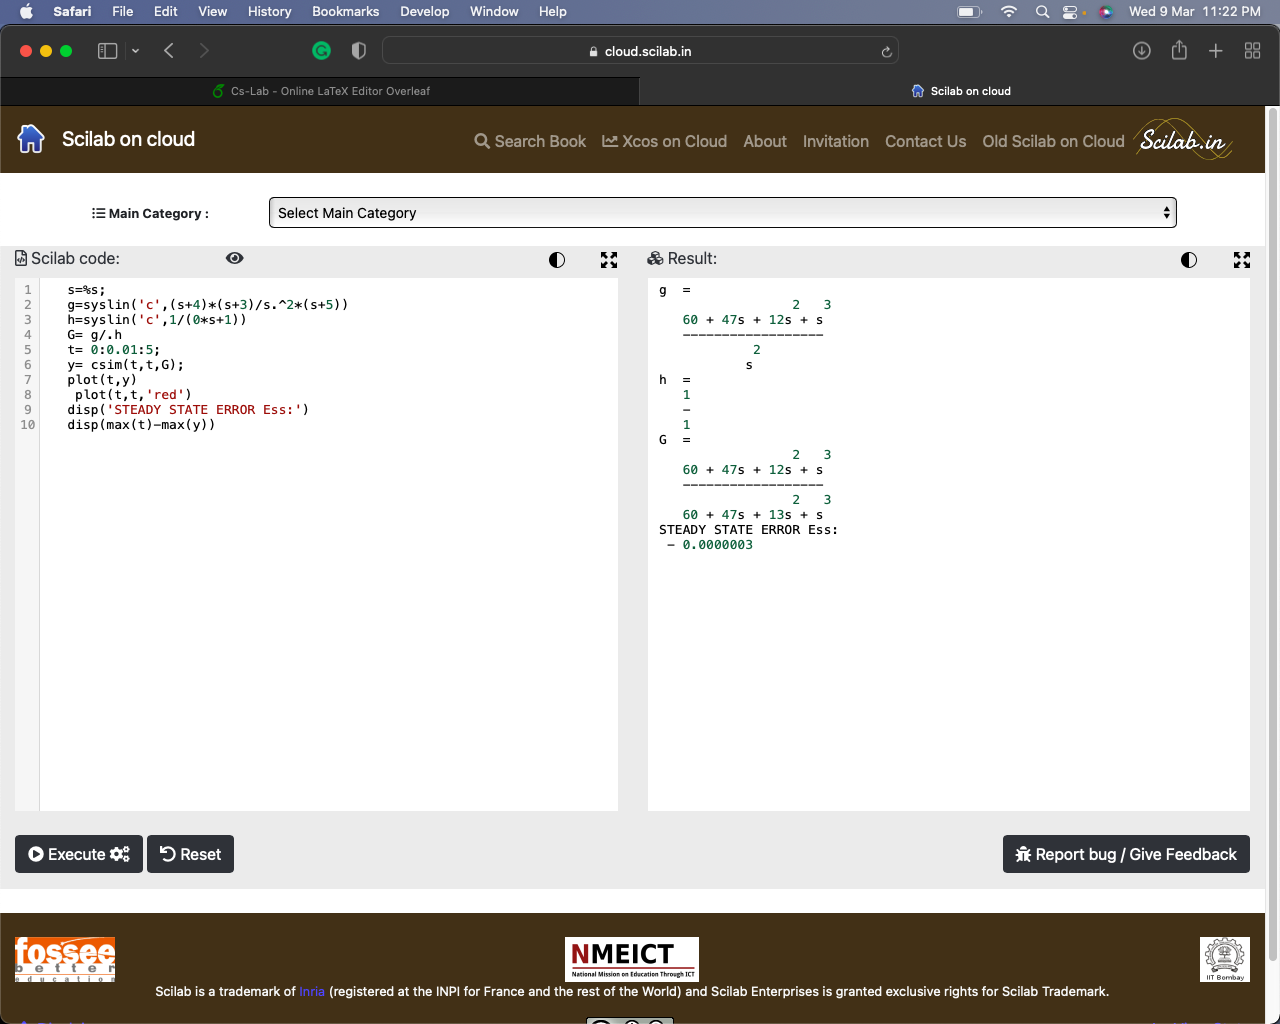
\includegraphics[width =10cm, height = 10cm]{images/exp82.png}
        \caption{Result}
        \label{Result}
\end{figure}

\section*{\textcolor{black}{Conclusion}}
 When we give a ramp input to type 2 system then we get 0 error as we increase the time.
     \pagebreak
\maketitle
\begin{center}
    \LARGE {EXPERIMENT NO : 9}
             
\end{center}

\section*{\textcolor{black}{AIM: }}
\text{To calculate steady state error in acceleration of Type 2}

\section*{\textcolor{black}{Block Diagram :}}

\begin{figure}[!hth]
        \centering
        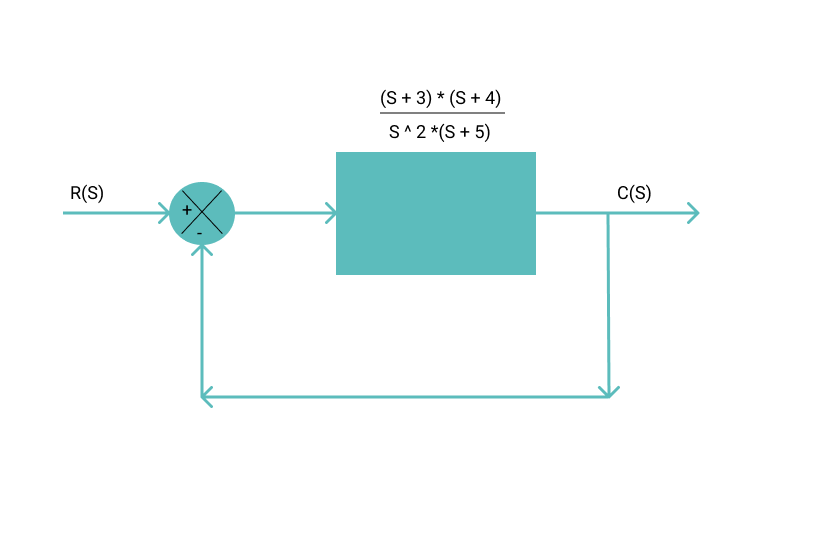
\includegraphics[width =10cm, height = 7cm]{images/exp9.png}
        \caption{Block Diagram}
        \label{Graph}
\end{figure}


\section*{\textcolor{black}{Theory :}}
Steady-state error is defined as the difference between the desired value and the actual value of a system output in the limit as time goes to infinity (i.e. when the response of the control system has reached steady-state).\par

Steady-state error is a property of the input/output response for a linear system. In general, a good control system will be one that has a low steady-state error
For a Type 0 system, the error is a non-zero, finite number, and Kp is equal to the Bode gain Kx. \par

\section*{\textcolor{black}{Code :}}

   s=\%s;\\ 
   g=syslin('c',(s+4)(s+3)/s.\wedge2(s+5))\\
   h=syslin('c',1/(0*s+1))\\
   G= g/.h\\
   t= 0:0.01:5;\\
   y= csim(t.\wedge2,t,G);\\
   plot(t,y)\\
    plot(t,t.\wedge2,'red')\\
   disp('STEADY STATE ERROR Ess:')\\
   disp(max(t.\wedge2)-max(y)) \par 

\section*{\textcolor{black}{OUTPUT/OBSERVATIONS}}

\begin{figure}[!hth]
        \centering
        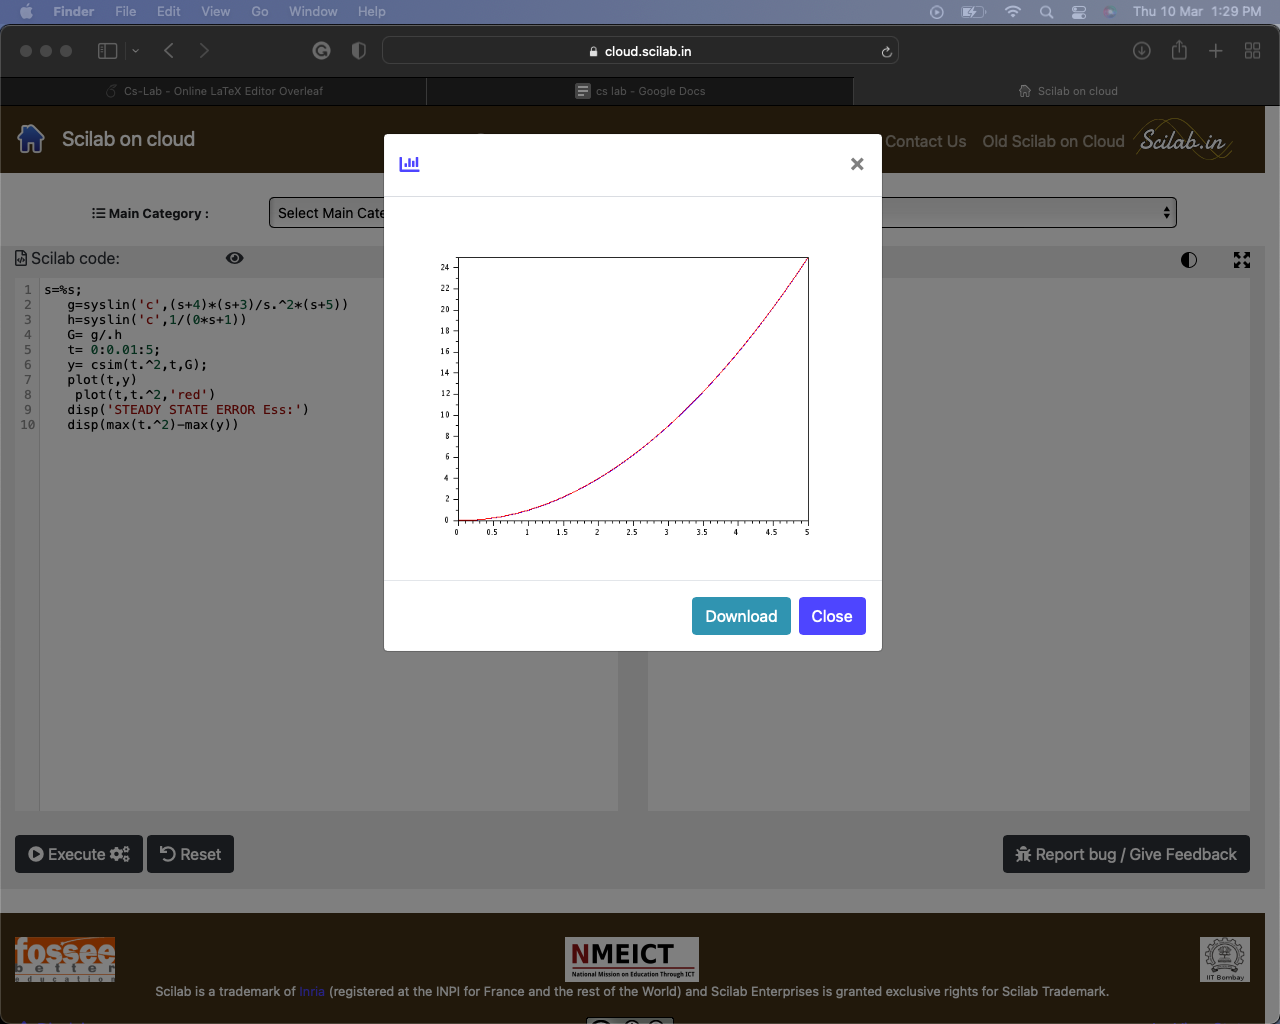
\includegraphics[width =10cm, height = 10cm]{images/exp91.png}
        \caption{Graph}
        \label{Graph}
\end{figure}
\begin{figure}[!hth]
        \centering
        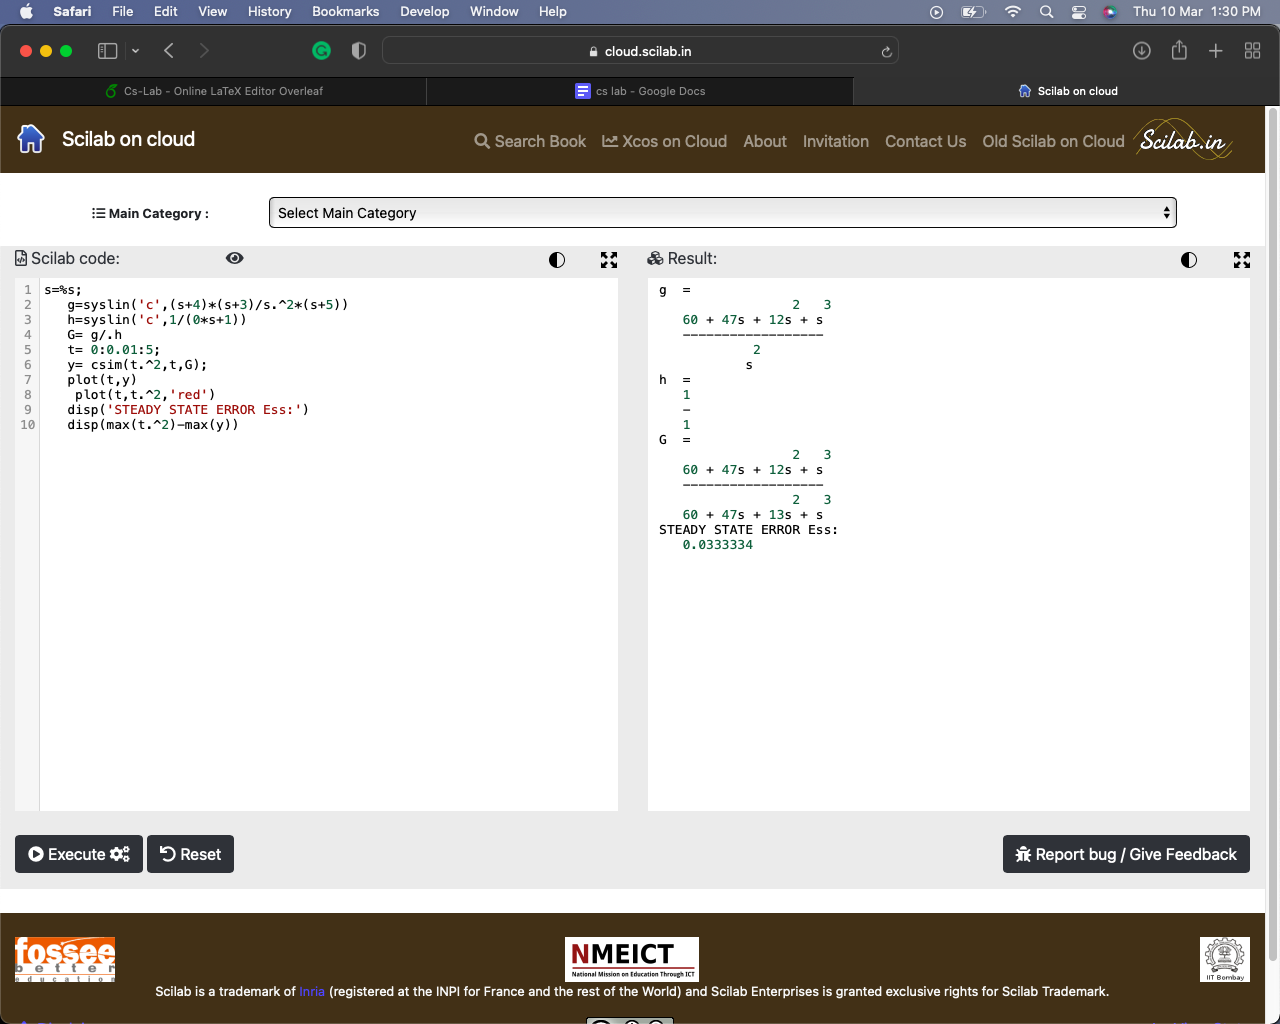
\includegraphics[width =10cm, height = 10cm]{images/exp92.png}
        \caption{Result}
        \label{Result}
\end{figure}

\section*{\textcolor{black}{Conclusion}}
After giving a parabolic input to type 2 system we get a constant error which is equal to 1/Ka.
 
 \pagebreak
 \begin{center}
    \LARGE {EXPERIMENT NO : 10}
             
\end{center}

\section*{\textcolor{black}{AIM:}}
\text{Calculating Transfer Function of Block Diagram by Reduction }

\section*{\textcolor{black}{Block Diagram :}}

\begin{figure}[!hth]
        \centering
        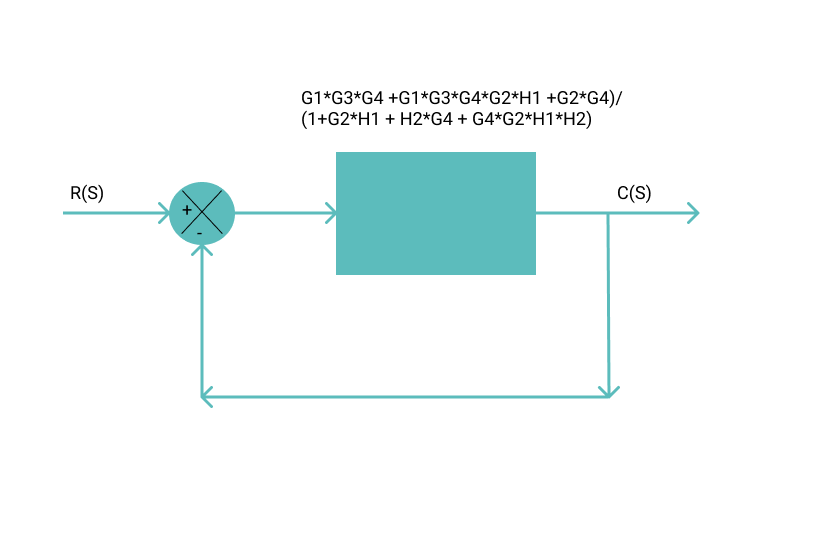
\includegraphics[width =10cm, height = 7cm]{images/Transfer funstion.png}
        \caption{Block Diagram}
        \label{Graph}
\end{figure}

\section*{\textcolor{black}{Theory :}}The gains in series are multiplied. And gain having a feedback having G(S) and H(s) is feedback gain .The combined value is given by $ G(S)/(1+H(S)*G(S)) $
 \par

\section*{\textcolor{black}{Code :}}
s=\%s;\\
g1= 10/(0*s +1);\\
G1 = syslin('c', g1);\\
g2=1/(s);\\
G2 = syslin('c', g2);\\
g3 = 1/(s+5);\\
G3 = syslin('c', g3);\\
g4= 2*s/(0*s+1);\\
G4 = syslin('c', g4);\\
h1 = 1/(s*0+1);\\
H1= syslin('c',h1);\\
h2= 1/s;\\
H2= syslin('c',h2);\\
//computing transfer function
Tmanual= (G1*G3*G4 +G1*G3*G4*G2*H1 +G2*G4)/(1+G2*H1 + H2*G4 + G4*G2*H1*H2);\\
disp('manually computed');\\
disp(Tmanual);\\
//computing using built-in commands
sub1=G1*G3;\\
sub2 = G2/.H1;\\
sub3 = G4/.H2;\\
sub4 = sub1 + sub2;\\
Tauto= sub4*sub3;\\
disp('auto computed');\\
disp(Tauto);\\ \par 

\section*{\textcolor{black}{OUTPUT/OBSERVATIONS}}

\begin{figure}[!hth]
        \centering
        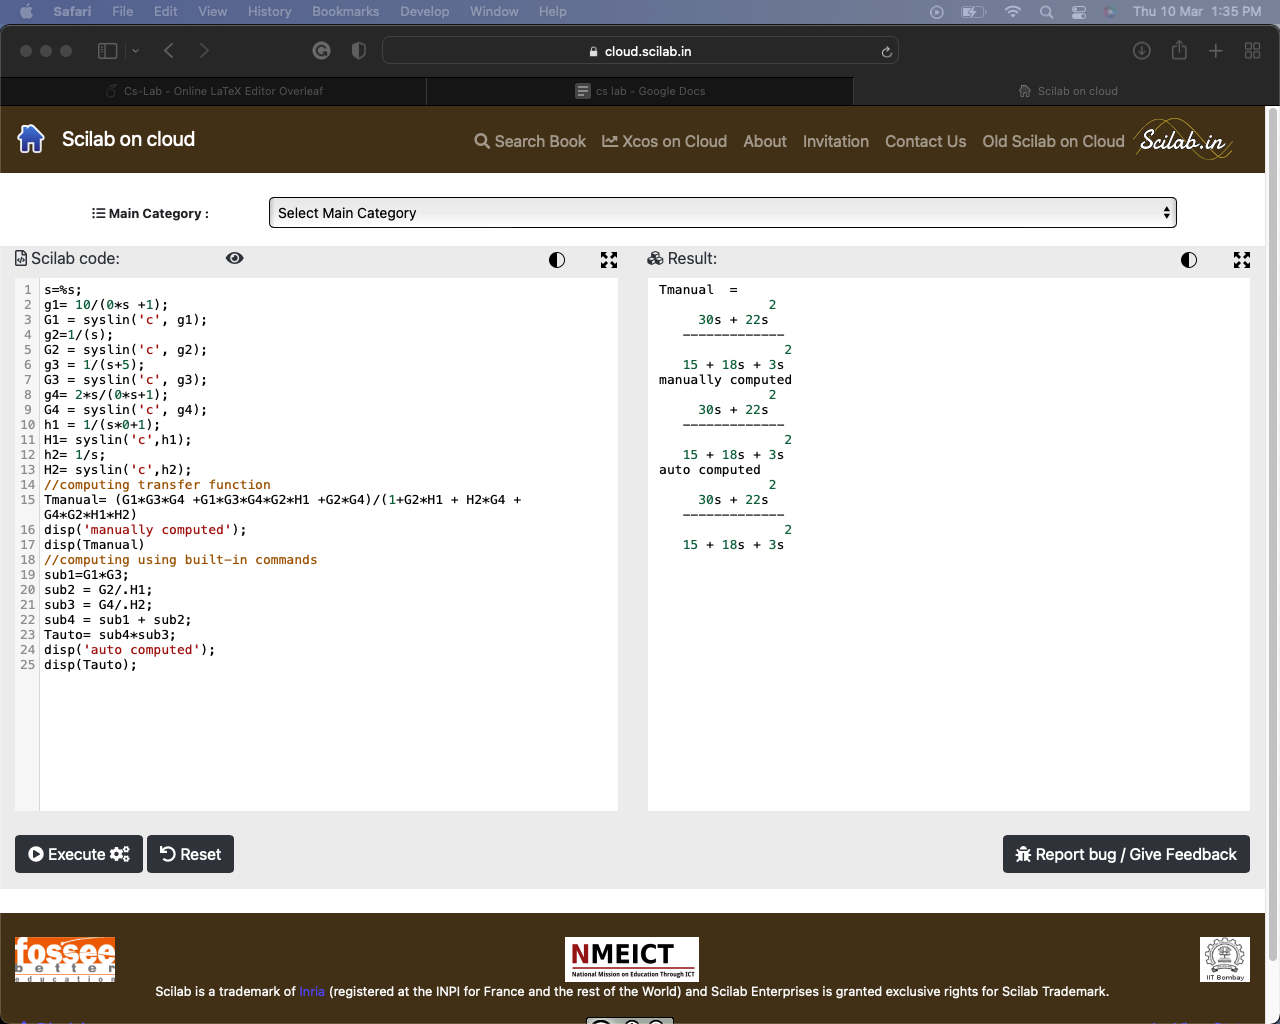
\includegraphics[width =10cm, height = 10cm]{images/exp101.png}
        \caption{Result}
        \label{Result}
\end{figure}


\section*{\textcolor{black}{Conclusion}}
It can be concluded that for complex block structures, block reduction tech- niques can be used to simplify the calculation and find our results without any error creeping in in our calculations.
 \pagebreak

 \begin{center}
    \LARGE {EXPERIMENT NO : 11}
             
\end{center}

\section*{\textcolor{black}{AIM: }}
\text{Speed Control in DC Motor}


\section*{\textcolor{black}{Block Diagram :}}

\begin{figure}[!hth]
        \centering
        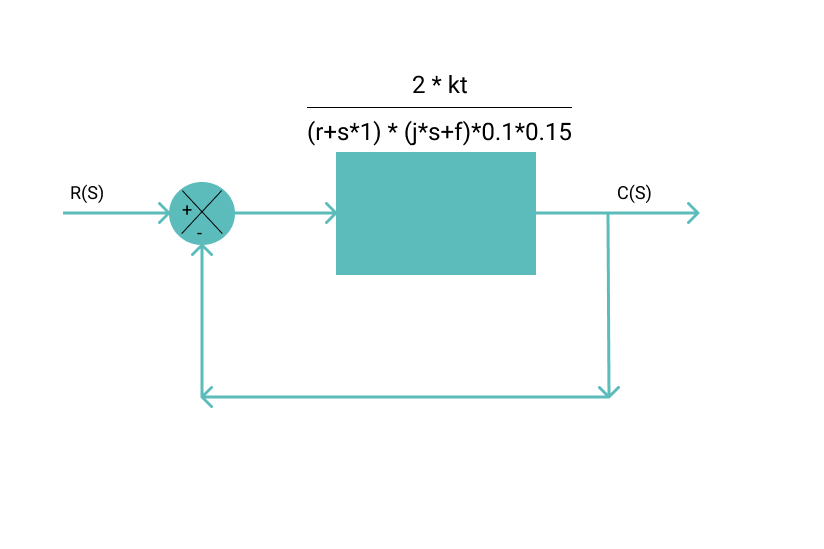
\includegraphics[width =10cm, height = 7cm]{images/speed control.png}
        \caption{Block Diagram}
        \label{Graph}
\end{figure}

\section*{\textcolor{black}{Theory :}}
We can control the speed of DC motor manually or through an automatic control device. This is different to speed regulation – where the speed can regulate against the natural change in speed due to a change in the load on the shaft.The speed of a DC motor (N) is equal to
N = K (V – IaRa)/ ø Where, K is a constant.

Thus, the speed of a DC motor can control in three ways;

-By varying the flux, and by varying the current through field winding
-By varying the armature voltage, and the armature resistance
-Through the supply voltage   
 \par

\section*{\textcolor{black}{Code :}}

  r=2;\\
l=0.5;\\
kt=0.1;   //magnetic flux\\
kb=0.1;\\
f=0.2;\\
j=0.02;\\
ka=2;       //f\\
ktm=0.15;  //feedback\\
 
s=\%s;\\
v2i=syslin('c',1/(r+s*1))\\
i2w=syslin('c',kt/(j*s+f))\\

dcm=v2i*i2w/.kb\\
tf=(ka*dcm)/.ktm\\
t=0:0.01:2;\\
ystep=csim('impulse',t,tf);\\

plot(t,ystep) \\\par 

\section*{\textcolor{black}{OUTPUT/OBSERVATIONS}}

\begin{figure}[!hth]
        \centering
        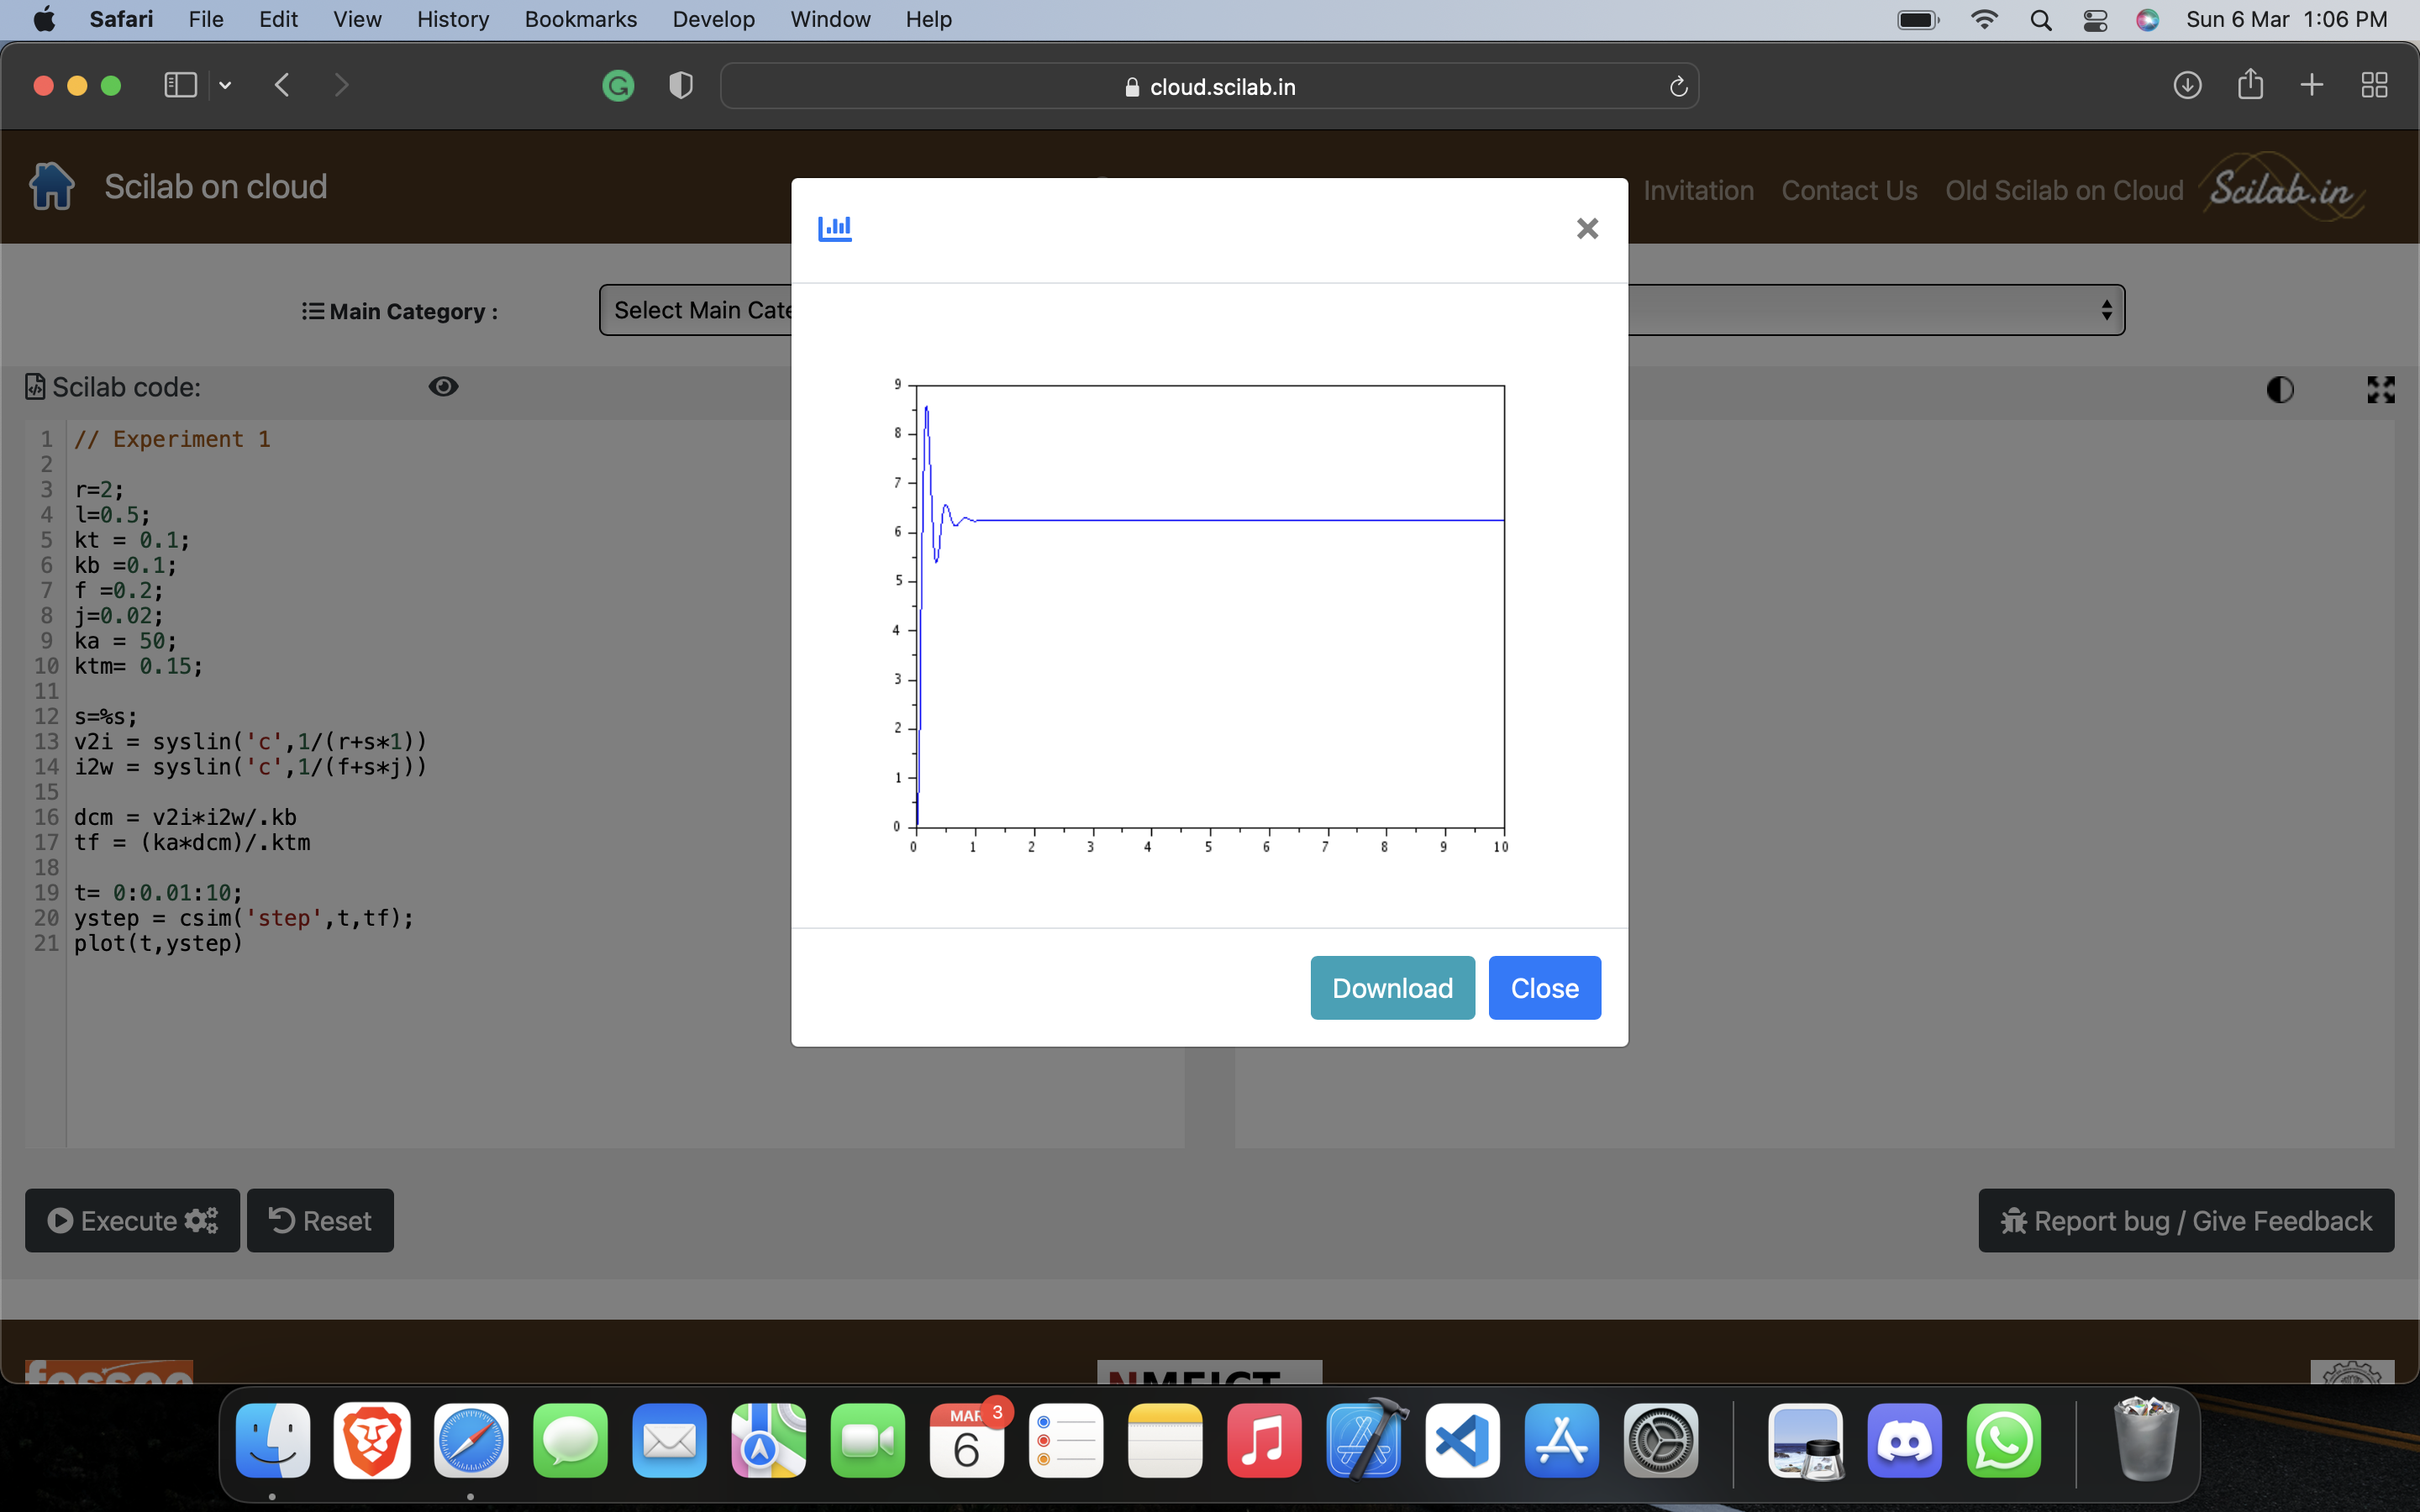
\includegraphics[width =10cm, height = 10cm]{images/Experiment1-output..png}
        \caption{Graph}
        \label{Graph}
\end{figure}
\begin{figure}[!hth]
        \centering
        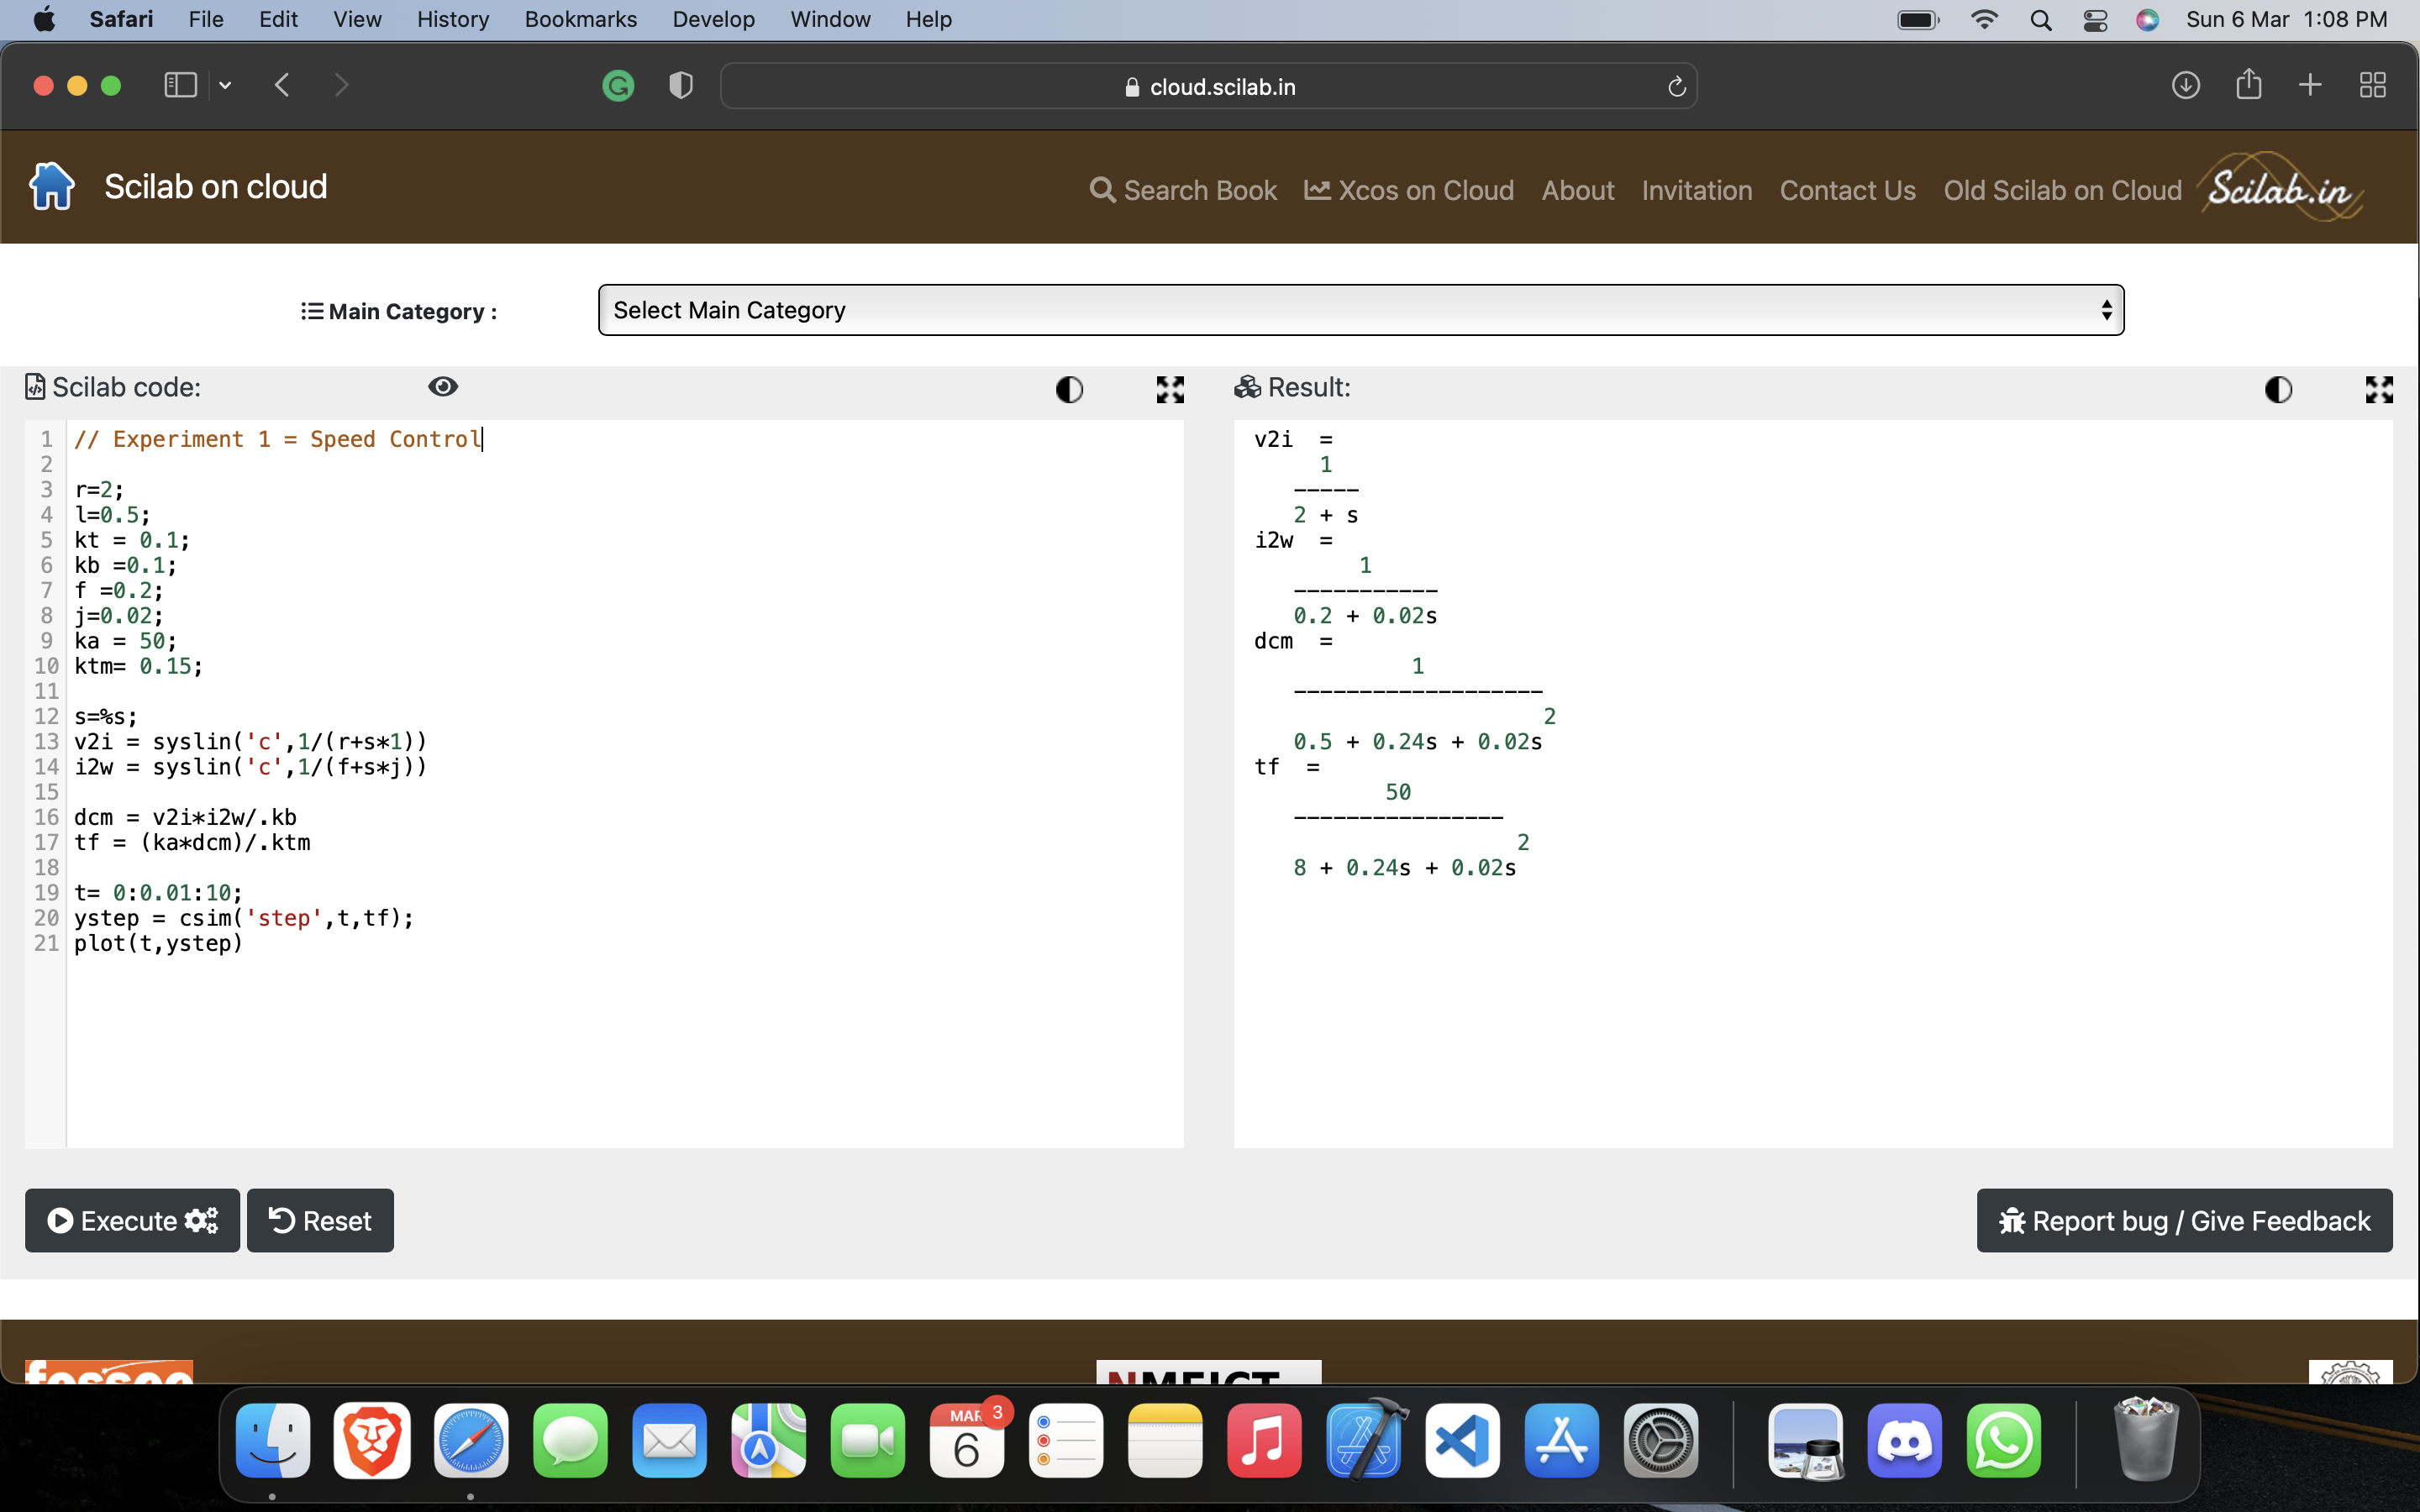
\includegraphics[width =10cm, height = 10cm]{images/Experiment1.png}
        \caption{Result}
        \label{Result}
\end{figure}

\section*{\textcolor{black}{Conclusion}}
From the above experiment, it can be concluded that various real world control systems can be realised and carefully calculated using control system tools. The speed control system of a motor can particularly be realised and its movements can be calculated by considering it as a second order system.
      
\pagebreak

\begin{center}
    \LARGE {EXPERIMENT NO : 12}
             
\end{center}

\section*{\textcolor{black}{AIM:}}
\text{Plotting Damping Factor and Wn values}

\section*{\textcolor{black}{Block Diagram :}}

\begin{figure}[!hth]
        \centering
        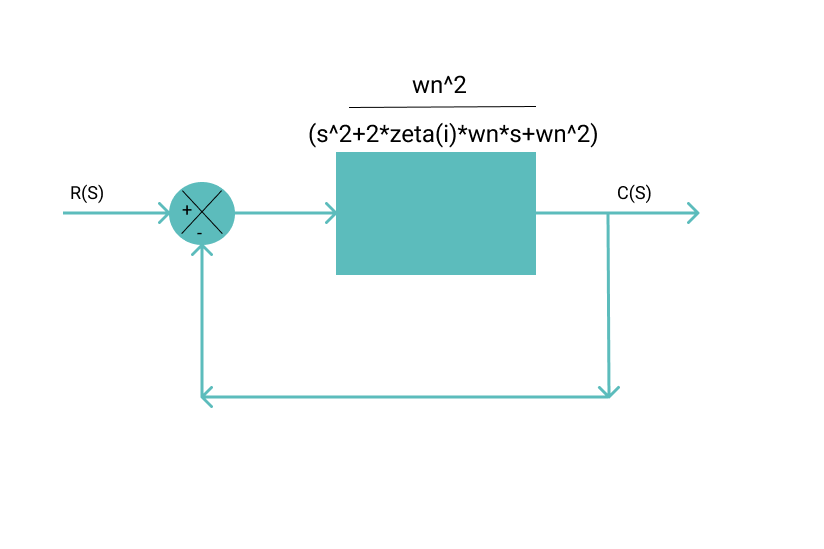
\includegraphics[width =10cm, height = 7cm]{images/damping factor.png}
        \caption{Block Diagram}
        \label{Graph}
\end{figure}

\section*{\textcolor{black}{Theory :}}
Plotting 2nd Order Time Response for different zeta values and a natural frequency value.Damping factor:
The damping ratio is defined as the number of oscillations in a system that can decay or restrain after an interruption and it is a dimensionless measurement. Most of the systems work in oscillatory mode when they are interrupted or disturbed from their initial position. For example, suspension of mass from a spring. If the mass is pulled and released, then it bounces up and down. The system tries to return to its initial static position after every bounce.
The damping ratio symbol is denoted as ‘ζ’ (Zeta).\par

\section*{\textcolor{black}{Code :}}
s= \%s;\\
zeta= [0 0.2 0.5 1 5 20];\\
wn=10;\\
col = ['r' 'b' 'g' 'b' 'r' 'g']\\
for i=1:6\\
     G=syslin('c',wn\wedge2/(s\wedge2+2*zeta(i)*wn*s+wn\wedge2))\\
     t=0:0.01:5;\\
     ystep=csim('step',t,G);\\
     plot(t,ystep,col(i));\\
end\\
   \par 

\section*{\textcolor{black}{OUTPUT/OBSERVATIONS}}

\begin{figure}[!hth]
        \centering
        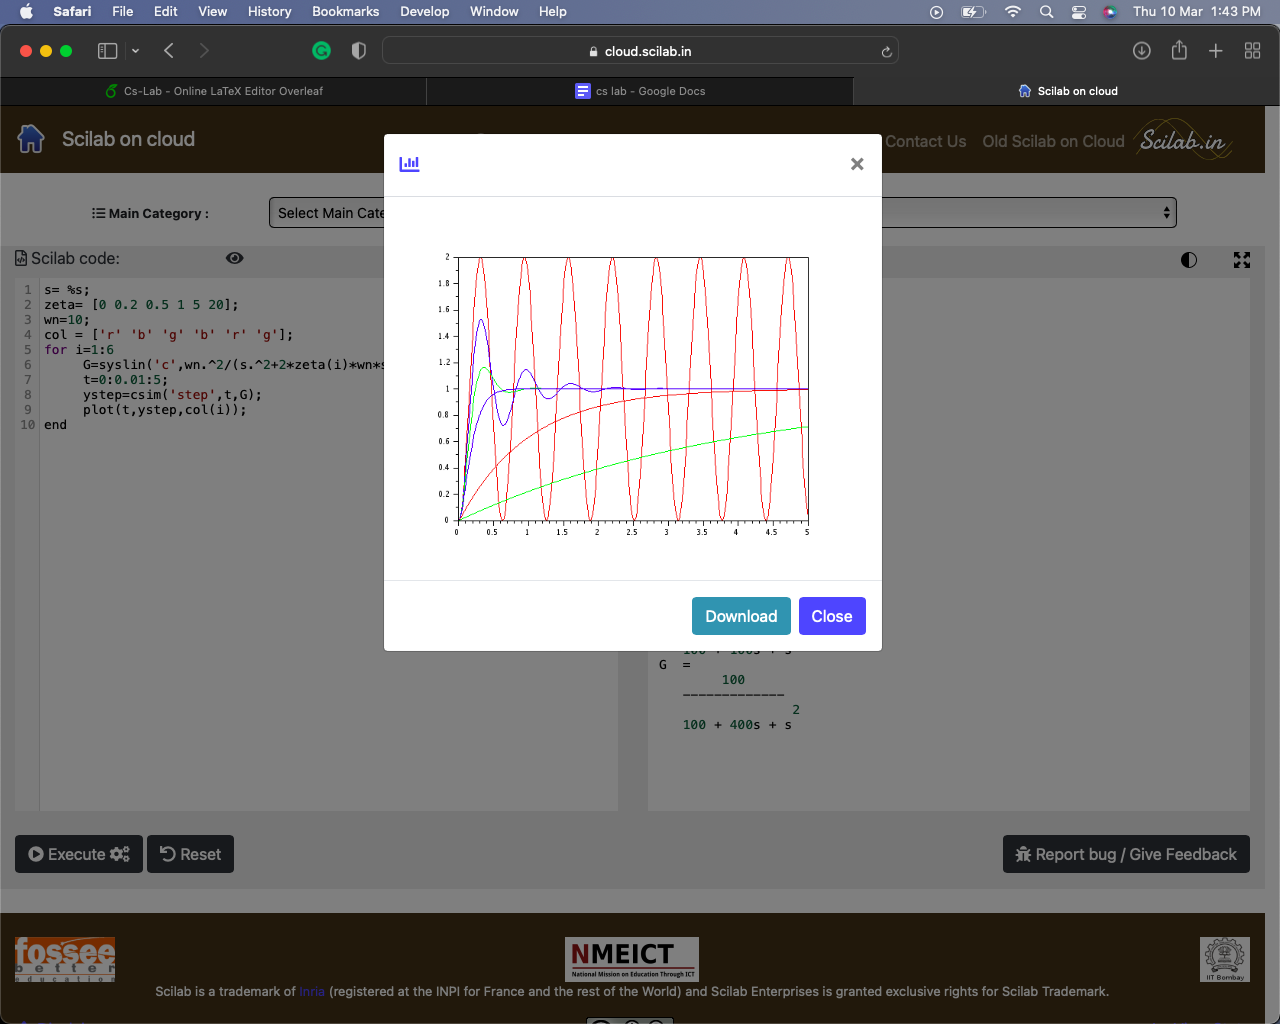
\includegraphics[width =10cm, height = 10cm]{images/exp121.png}
        \caption{Graph}
        \label{Graph}
\end{figure}
\begin{figure}[!hth]
        \centering
        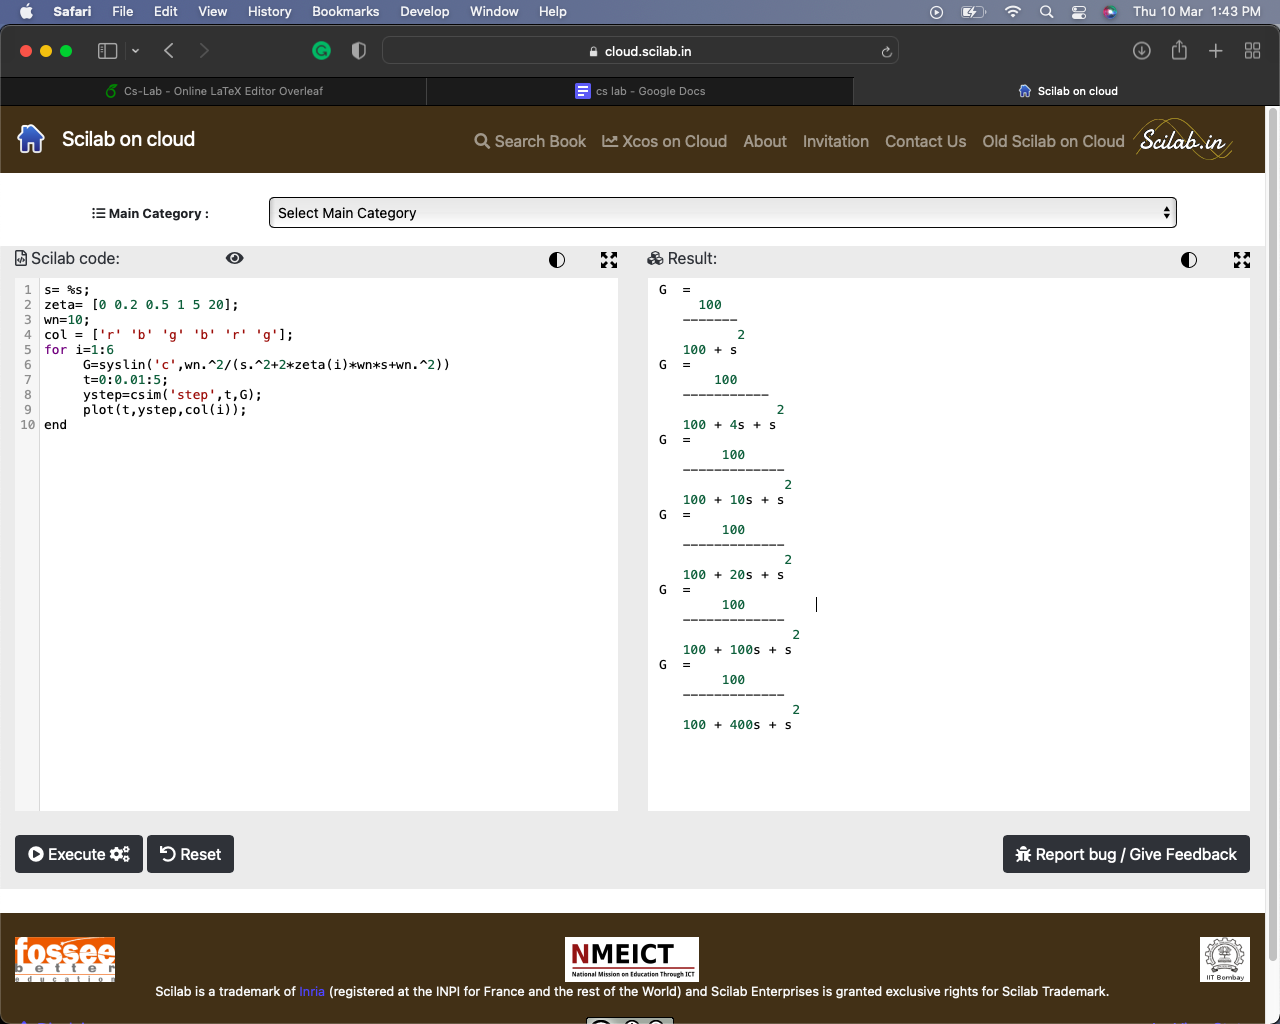
\includegraphics[width =10cm, height = 10cm]{images/exp122.png}
        \caption{Result}
        \label{Result}
\end{figure}

\section*{\textcolor{black}{Conclusion}}
From the above experiment, it can be concluded that for getting a desired output, we should consider the value of zeta between zero and one. This way, we get our system output in less time with few inconsistencies in the beginning.
 
 \pagebreak


\begin{center}
    \LARGE {EXPERIMENT NO : 13}
             
\end{center}

\section*{\textcolor{black}{AIM: }}
\text{Plot poles using different zeta values}

\section*{\textcolor{black}{Block Diagram :}}

\begin{figure}[!hth]
        \centering
        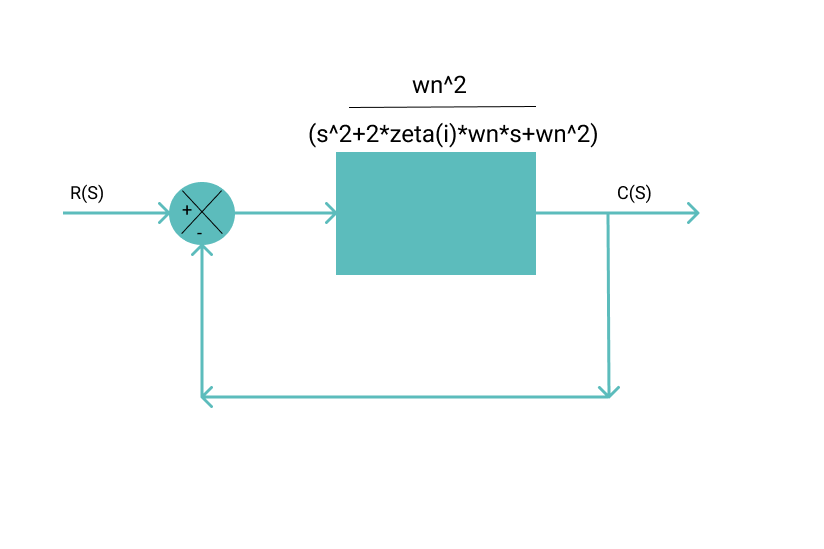
\includegraphics[width =10cm, height = 7cm]{images/damping factor.png}
        \caption{Block Diagram}
        \label{Graph}
\end{figure}

\section*{\textcolor{black}{Theory :}}
POLES:The values for which the equation in denominator for a transfer function is Zero.
 Zeta = Damping factor of 2nd order Time Response 
  wn =natural frequency.
zeta — Damping ratio of each pole
Damping ratios of each pole, returned as a vector sorted in the same order as wn .If sys is a discrete-time model with specified sample time, zeta contains the damping ratios of the equivalent continuous-time poles
 \par

\section*{\textcolor{black}{Code :}}
s= \%s;\\
zeta= [0 0.2 0.5 1 5 20];\\
wn=10;\\
col = ['r' 'b' 'g' 'b' 'r' 'g']\\
for i=1:6\\
     G=syslin('c',(wn)\wedge2/(s\wedge2+2*zeta(i)*wn*s+(wn)\wedge2))\\
     plzr(G)\\
end\\

   \par 

\section*{\textcolor{black}{OUTPUT/OBSERVATIONS}}

\begin{figure}[!hth]
        \centering
        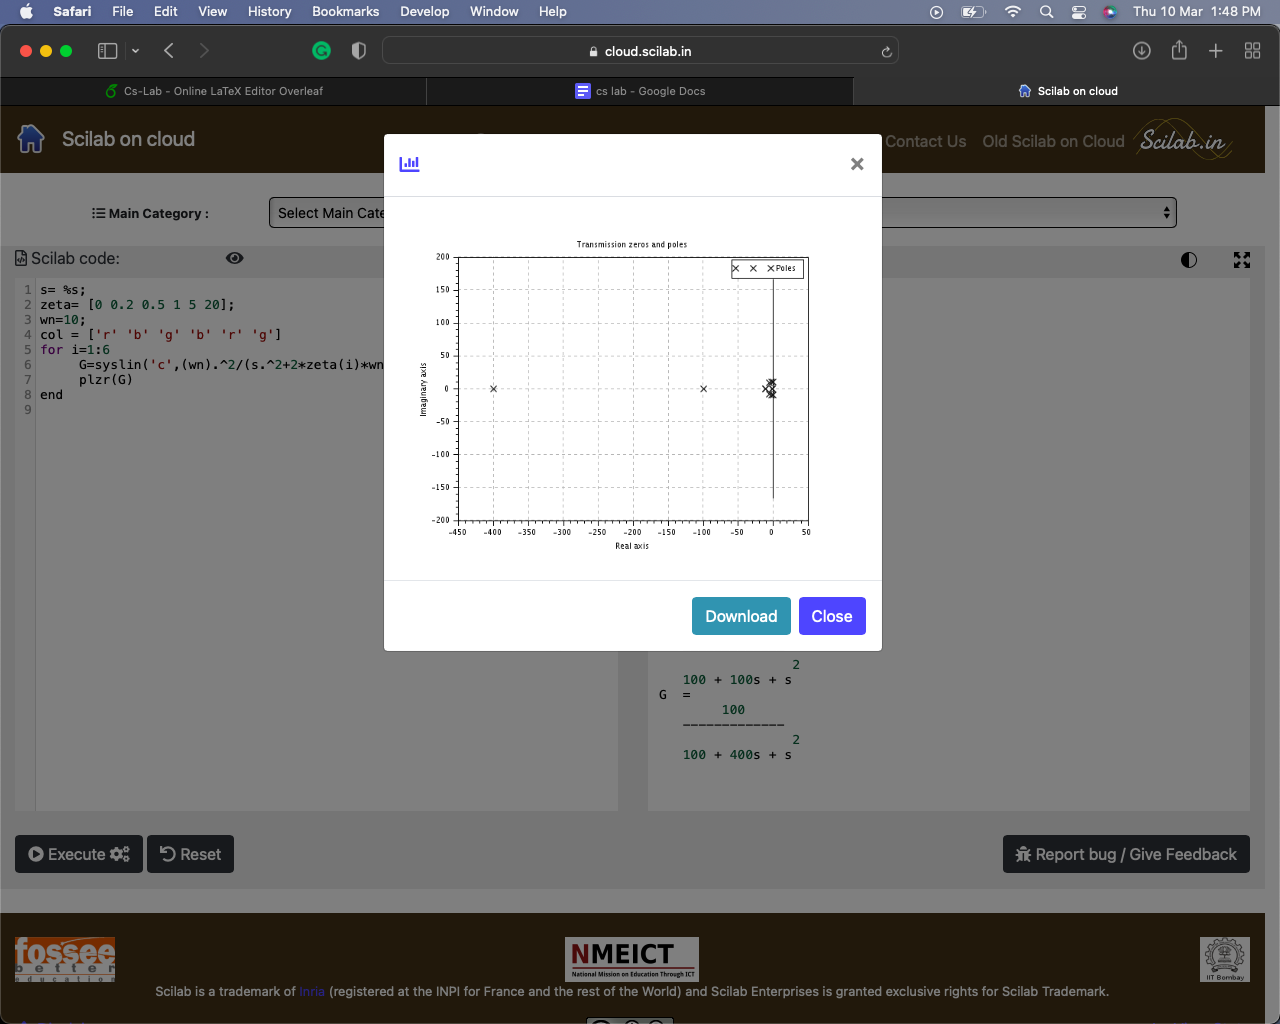
\includegraphics[width =10cm, height = 10cm]{images/exp131.png}
        \caption{Graph}
        \label{Graph}
\end{figure}

\begin{figure}[!hth]
        \centering
        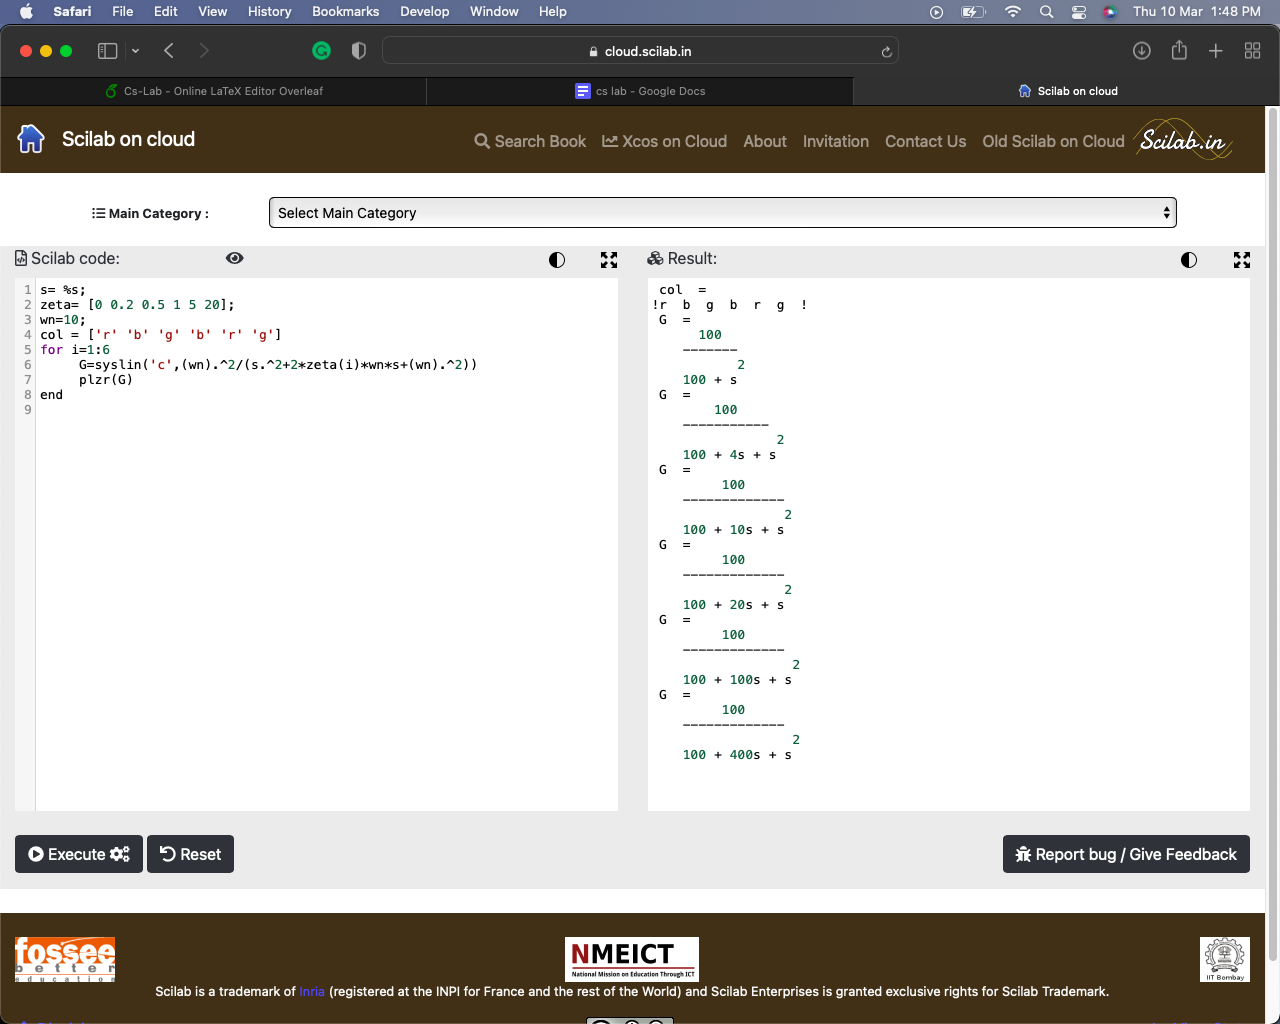
\includegraphics[width =10cm, height = 10cm]{images/exp132.png}
        \caption{Graph}
        \label{Result}
\end{figure}
\section*{\textcolor{black}{Conclusion}}
From the above analysis, it can be concluded that the closed-loop systems tend to be stable under certain conditions. the mere fact that all closed-loop poles lie in the left-half s plane does not guarantee satisfactory transient- response characteristics. If dominant complex-conjugate closed-loop poles lie close to the j axis, the transient response may exhibit excessive oscillations or may be very slow. Therefore, to guarantee fast, yet well-damped, transient-response characteristics, it is necessary that the closed-loop poles of the system lie in a particular region in the complex plane.
 \pagebreak


\begin{center}
    \LARGE {EXPERIMENT NO : 14}
             
\end{center}

\section*{\textcolor{black}{AIM: }}
\text{To find out the unstable roots in a system without calculating for it by using the routh stability criterion}

\section*{\textcolor{black}{Block Diagram :}}

\begin{figure}[!hth]
        \centering
        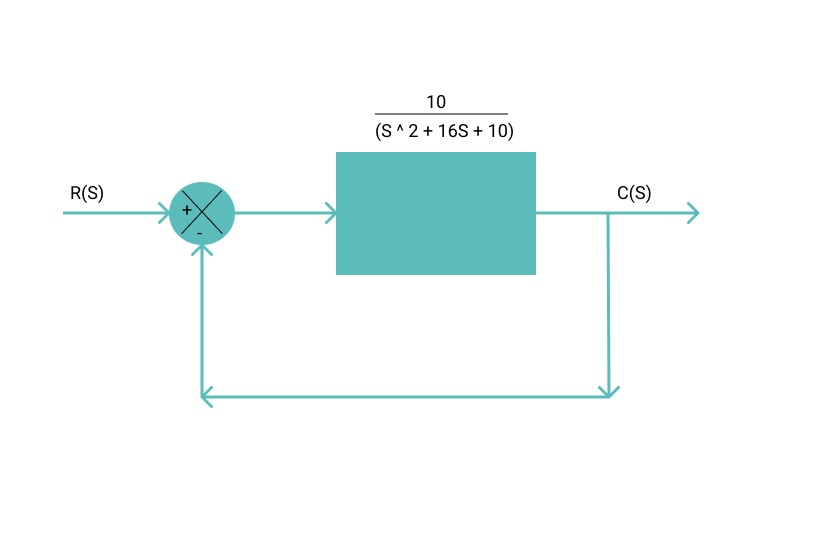
\includegraphics[width =10cm, height = 7cm]{images/exp141.png}
        \caption{Block Diagram}
        \label{Graph}
\end{figure}

\section*{\textcolor{black}{Theory :}}
Routh’s stability criterion tells us whether or not there are unstable roots in a polynomial equation without actually solving for them. This stability criterion applies to polynomials with only a finite number of terms. When the criterion is applied to a control system, information about absolute stability can be obtained directly from the coefficients of the characteristic equation.
To find the Routh’s stability criterion, we take the following steps:
1. Write the polynomial in s in the following form:
           
where the coefficients are real quantities. We assume that ; that is, any zero root has been removed. 
2. If any of the coefficients are zero or negative in the presence of at least one positive coefficient, a root or roots exist that are imaginary or that have positive real parts. Therefore, in such a case, the system is not stable.
3. If all coefficients are positive, arrange the coefficients of the polynomial in rows and columns according.

Here,  ,  and so on. Similarly, we can find c.
This process is continued until the nth row has been completed.Routh’s stability criterion states that the number of roots of characteristic equation with positive real parts is equal to the number of changes in sign of the coefficients of the first column of the array. It should be noted that the exact values of the terms in the first column need not be known; instead, only the signs are needed.
 \par

\section*{\textcolor{black}{Code :}}
s = \%s;\\
oltf= syslin('c',10/(s\wedge2+16*s+16))\\
fb=syslin('c',1/(0*s+1))\\
cltf = oltf/.fb\\
\texttt{[R\underline{{ }}arr,n]=routh\underline{{ }}t(denom(cltf))}\\
plzr(cltf)\\
   \par 

\section*{\textcolor{black}{OUTPUT/OBSERVATIONS}}

\begin{figure}[!hth]
        \centering
        \includegraphics[width =10cm, height = 10cm]{images/exp142.png}
        \caption{Graph}
        \label{Graph}
\end{figure}


\section*{\textcolor{black}{Observation and Conclusion}}
In the output we can see that in the first column of the Routh array there is no sign change and also no missing term or 0 term hence the given system is stable. If all the roots of the characteristic equation exist to the left half of the ‘s’ plane, then  system is stable. If at least one root of the characteristic equation exists to the right half of the ‘s’ plane, then  system is unstable.

 \pagebreak
 
 \begin{center}
    \LARGE {EXPT 15:Root Locus}
             
\end{center}

\section*{\textcolor{black}{AIM: }}
\text{To understand and find the root loci of a given system.}

\section*{\textcolor{black}{Block Diagram :}}

\begin{figure}[!hth]
        \centering
        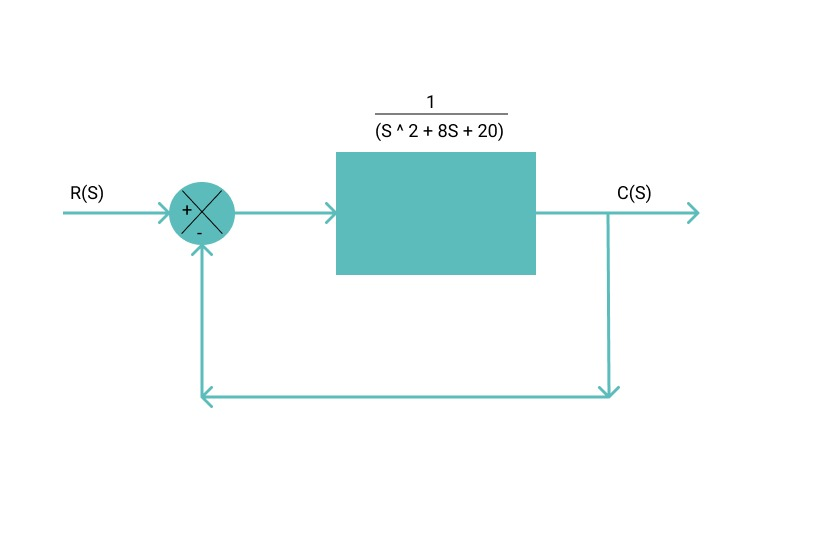
\includegraphics[width =20cm, height = 10cm]{images/root block.jpeg}
        \caption{Graph}
        \label{Graph}
\end{figure}

\section*{\textcolor{black}{Theory :}}
The root loci for the system are the loci of the closed-loop poles as the gain K is varied from zero to infinity.
A typical procedure for sketching the root-locus plot is as follows:\\
1. Determine the root loci on the real axis.\\
2. Determine the asymptotes of the root loci.\\
3. Determine the breakaway point.\\
4. Determine the points where the root loci cross the imaginary axis.\\
5. Choose a test point in the broad neighborhood of the jw axis and origin.\\
6. Draw the root loci, based on the information obtained.\\

 \par

\section*{\textcolor{black}{Code :}}
///Code 1
s=\%s;\\
g=syslin('c',1/((s.\wedge2+8*s+20)))\\
plzr(g)\\
sgrid()\\

///Code 2

s=\%s;\\
g=syslin('c',1/((s.\wedge2+8*s+20)))\\
plzr(g)\\
sgrid()\\

  \par 

\section*{\textcolor{black}{OUTPUT}}

\begin{figure}[!hth]
        \centering
        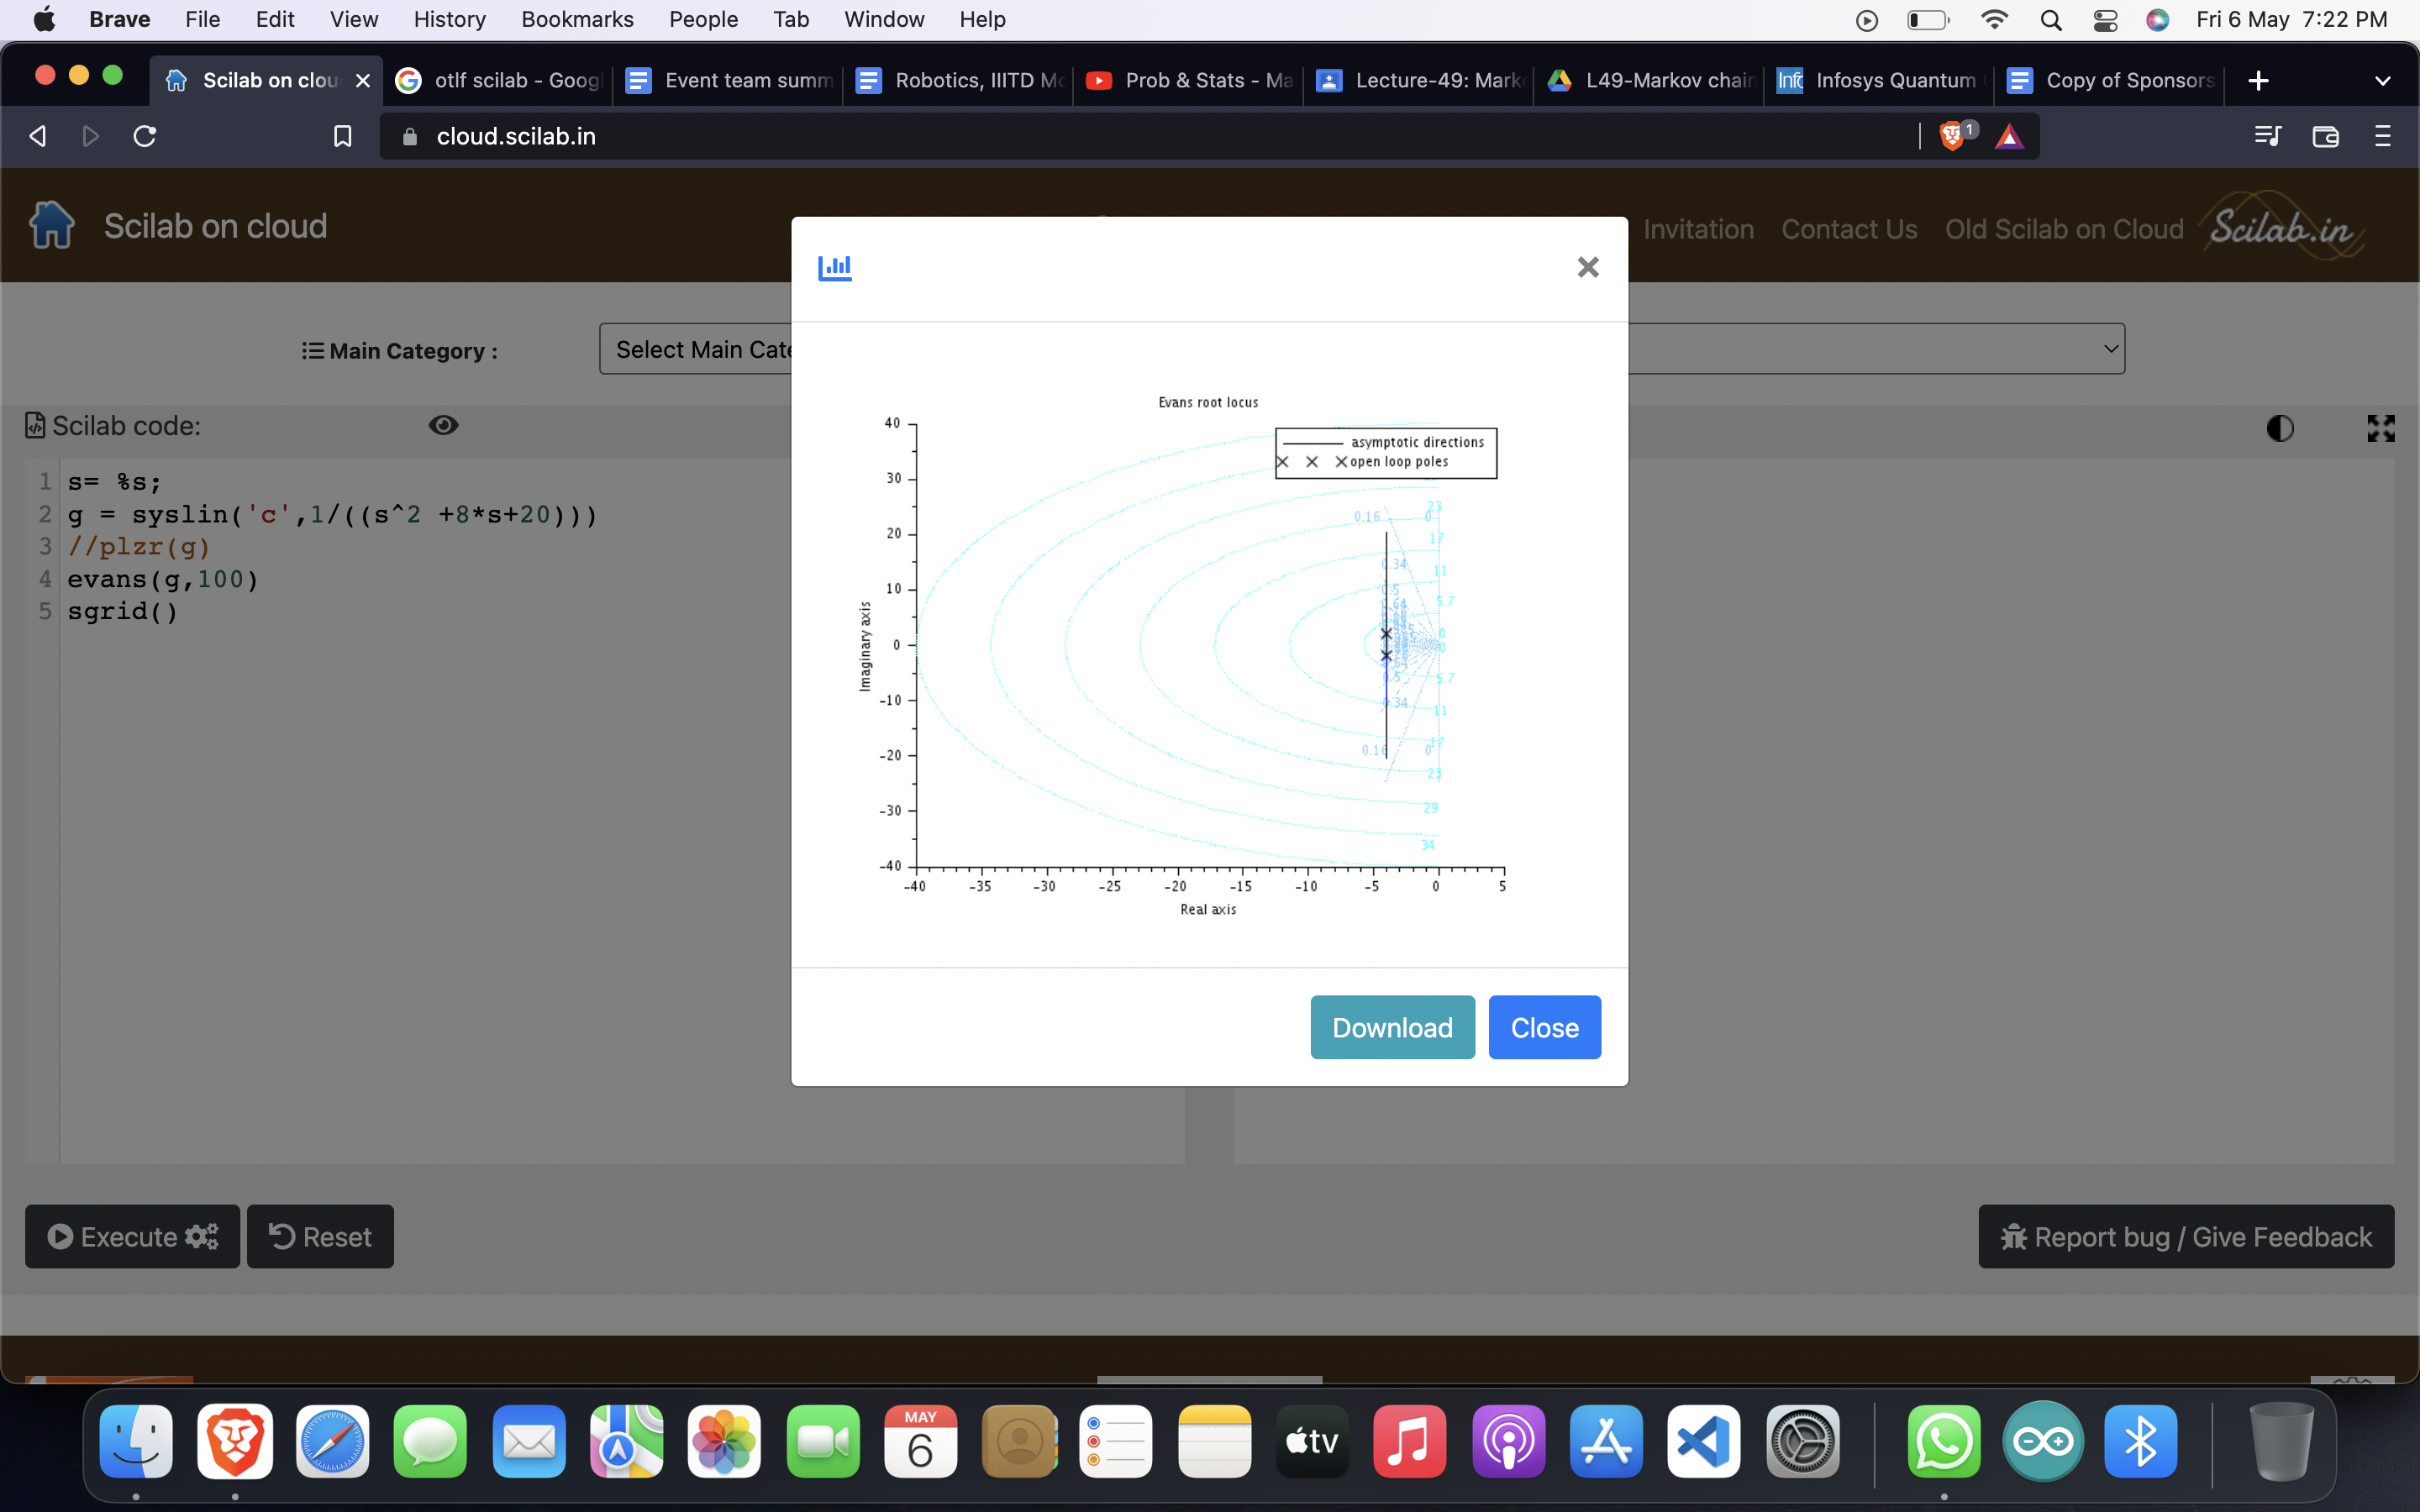
\includegraphics[width =20cm, height = 10cm]{images/exp151.png}
        \caption{Graph}
        \label{Graph}
\end{figure}
\begin{figure}[!hth]
        \centering
        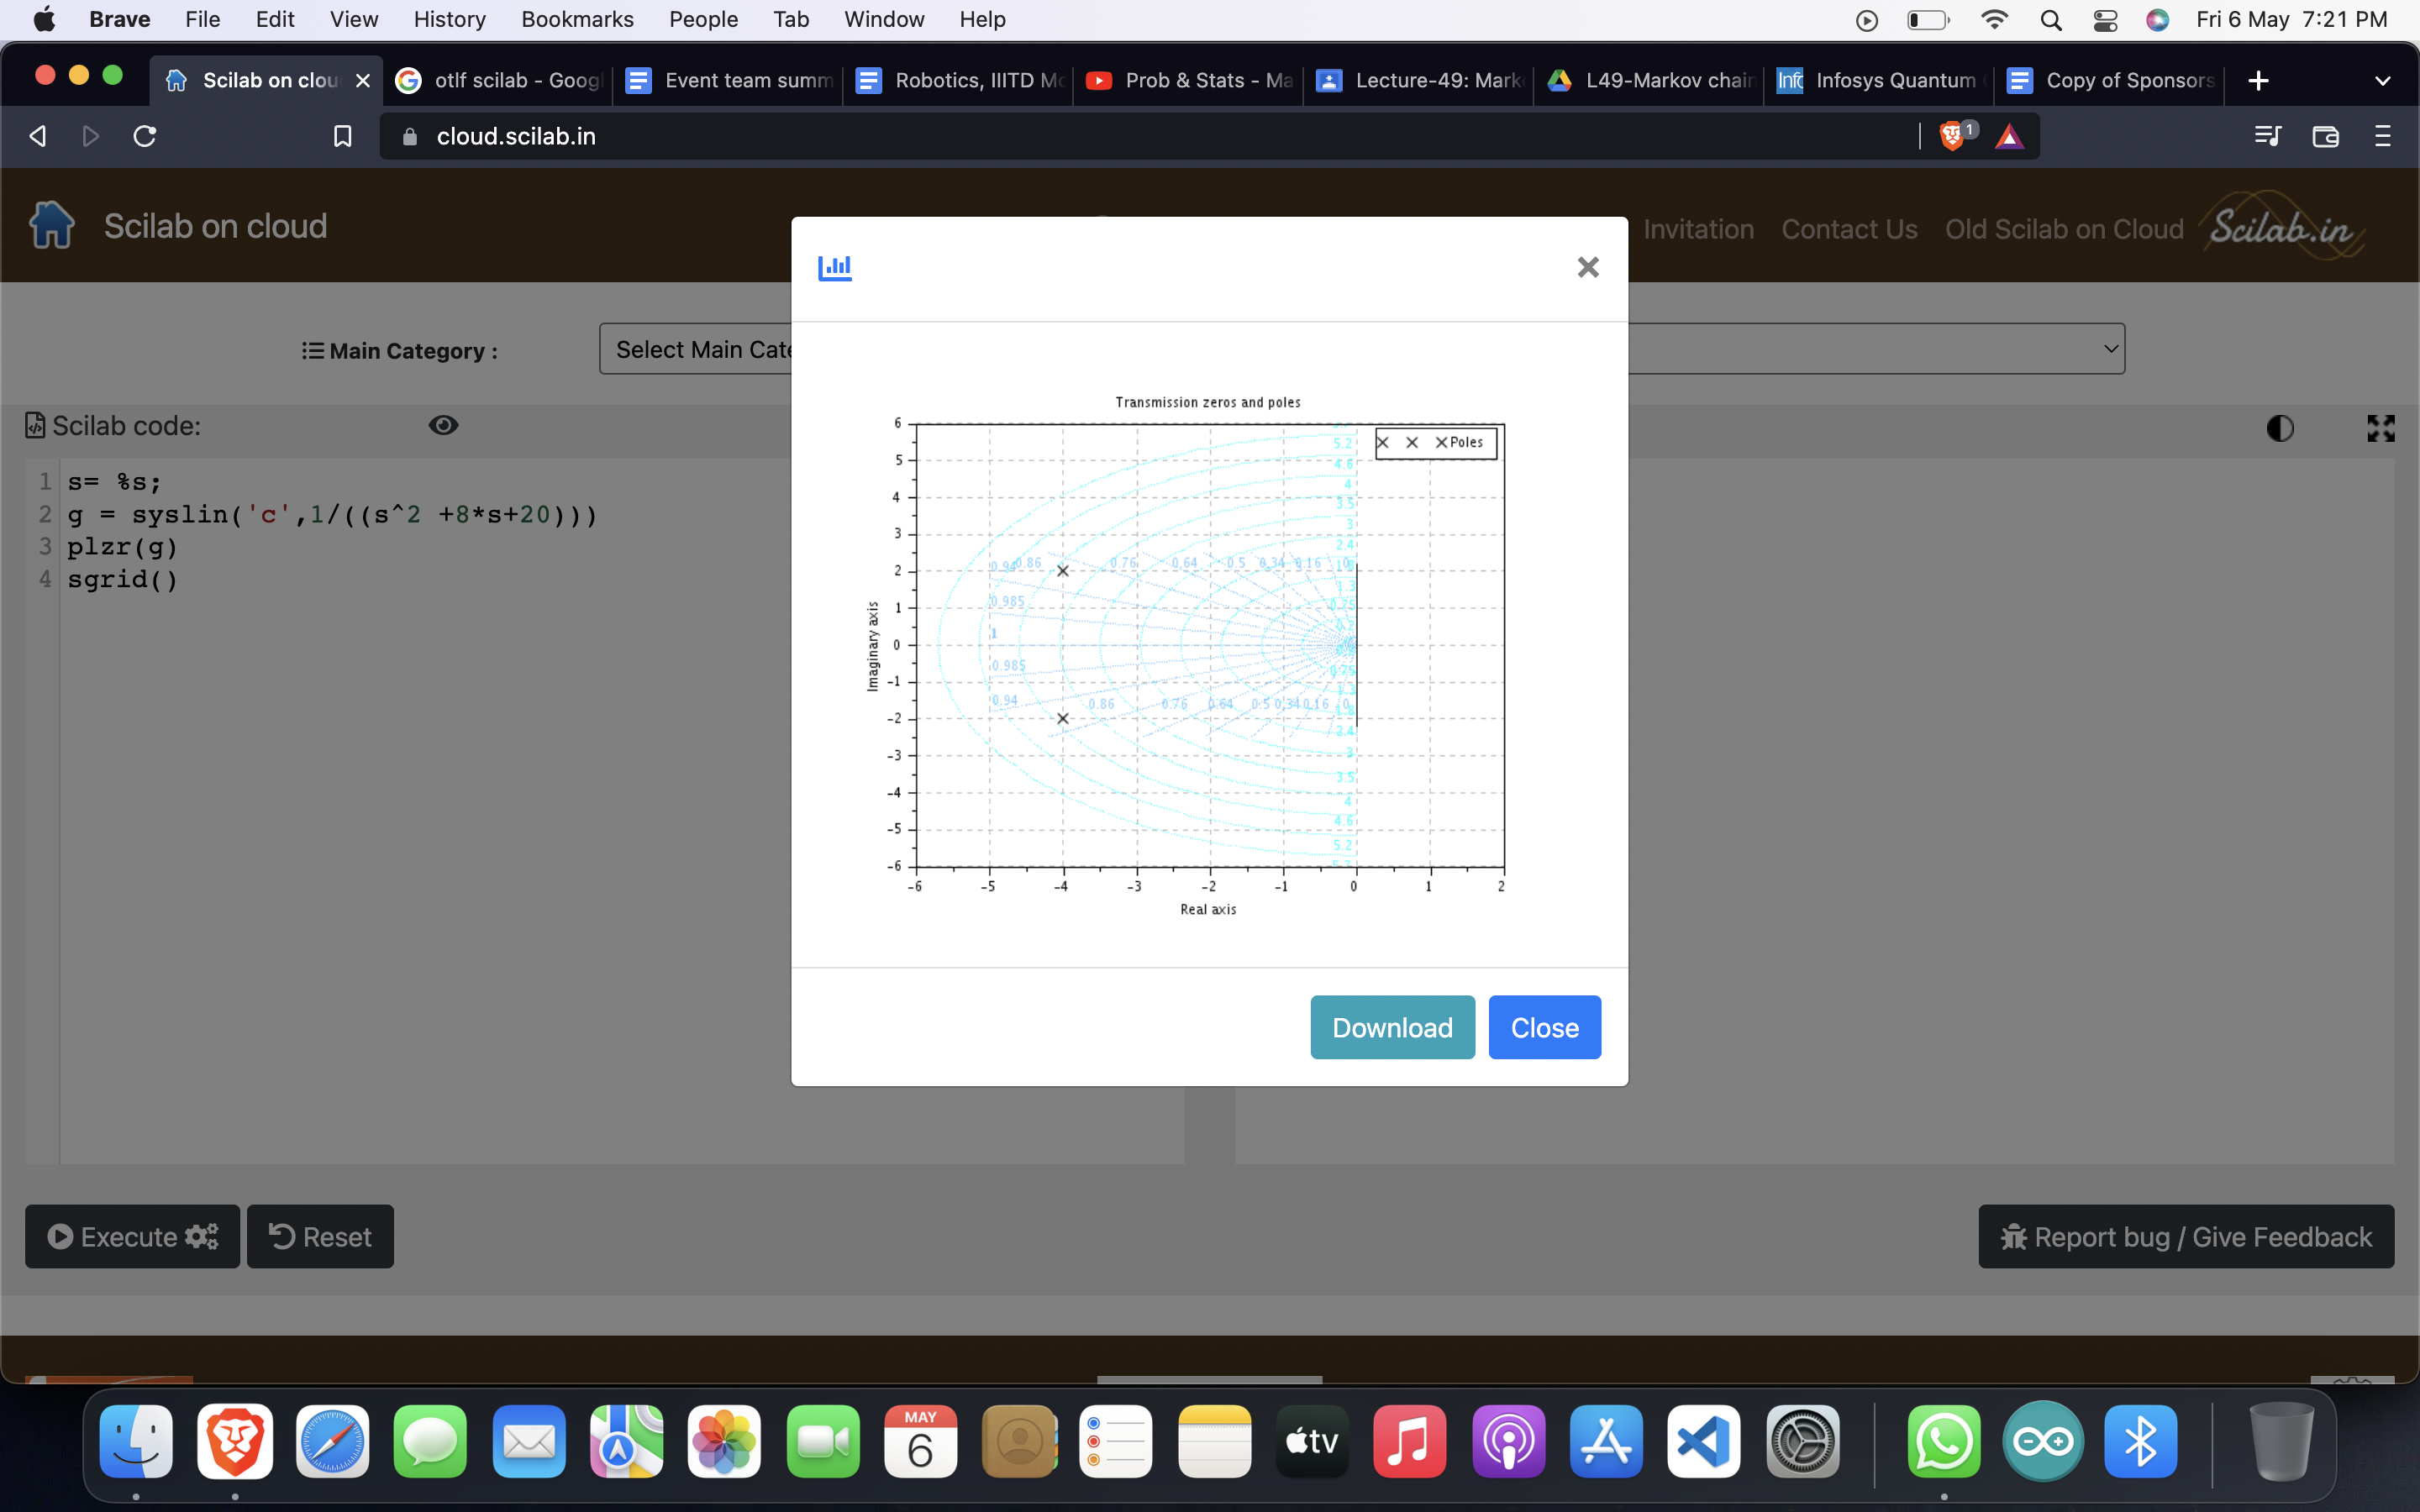
\includegraphics[width =20cm, height = 10cm]{images/exp152.png}
        \caption{Graph}
        \label{Graph}
\end{figure}

\section*{\textcolor{black}{Observation and Conclusion}}
The root locus starts at oltf poles and ends at the oltf zeroes.
\pagebreak
 
 
 
\begin{center}
    \LARGE {EXPT 16:Bode Plot}
             
\end{center}

\section*{\textcolor{black}{AIM: }}
\text{To understand the stability of a system using its Bode plot.}

\section*{\textcolor{black}{Block Diagram :}}

\begin{figure}[!hth]
        \centering
        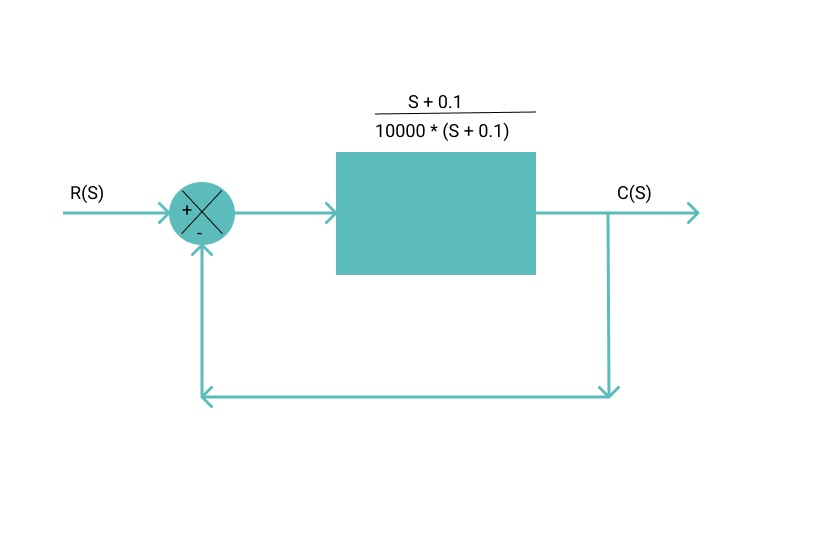
\includegraphics[width =20cm, height = 10cm]{images/bode block 1.jpeg}
        \caption{Graph}
        \label{Graph}
\end{figure}
\begin{figure}[!hth]
        \centering
        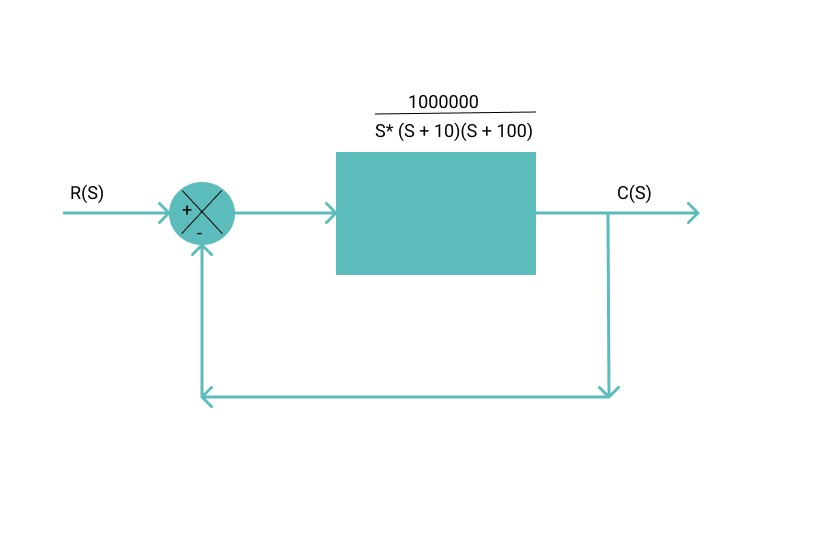
\includegraphics[width =20cm, height = 10cm]{images/bode block 2.jpeg}
        \caption{Graph}
        \label{Graph}
\end{figure}


\section*{\textcolor{black}{Theory :}}
A Bode diagram consists of two graphs: One is a plot of the logarithm of the magnitude of a sinusoidal transfer function; the other is a plot of the phase angle; both are plotted against the frequency on a logarithmic scale. The standard representation of the logarithmic magnitude of G(jw) is , where the base of the logarithm is 10.The unit used in this representation of the magnitude is the decibel, usually abbreviated dB.

The magnitude of the open loop transfer function in dB is -
  M=20log|G(jω)H(jω)|

The phase angle of the open loop transfer function in degrees is -
  ϕ=∠G(jω)H(jω)

 \par

\section*{\textcolor{black}{Code :}}

s = \%s;\\
p = syslin('c',1000000/(s*(s*1+10)*(s*1+ 100)))\\
h = syslin('c', (s*1+0.1)/(10000*(s*1+0.1)))\\
g = p*h \\        
bode(g)\\
bode(h)\\
bode(p)\\
\texttt{g\underline{{ }}margin(g)}\\
\texttt{p\underline{{ }}margin(g)}\\
\texttt{show\underline{{ }}margins(g)}\\


  \par 

\section*{\textcolor{black}{OUTPUT}}

\begin{figure}[!hth]
        \centering
        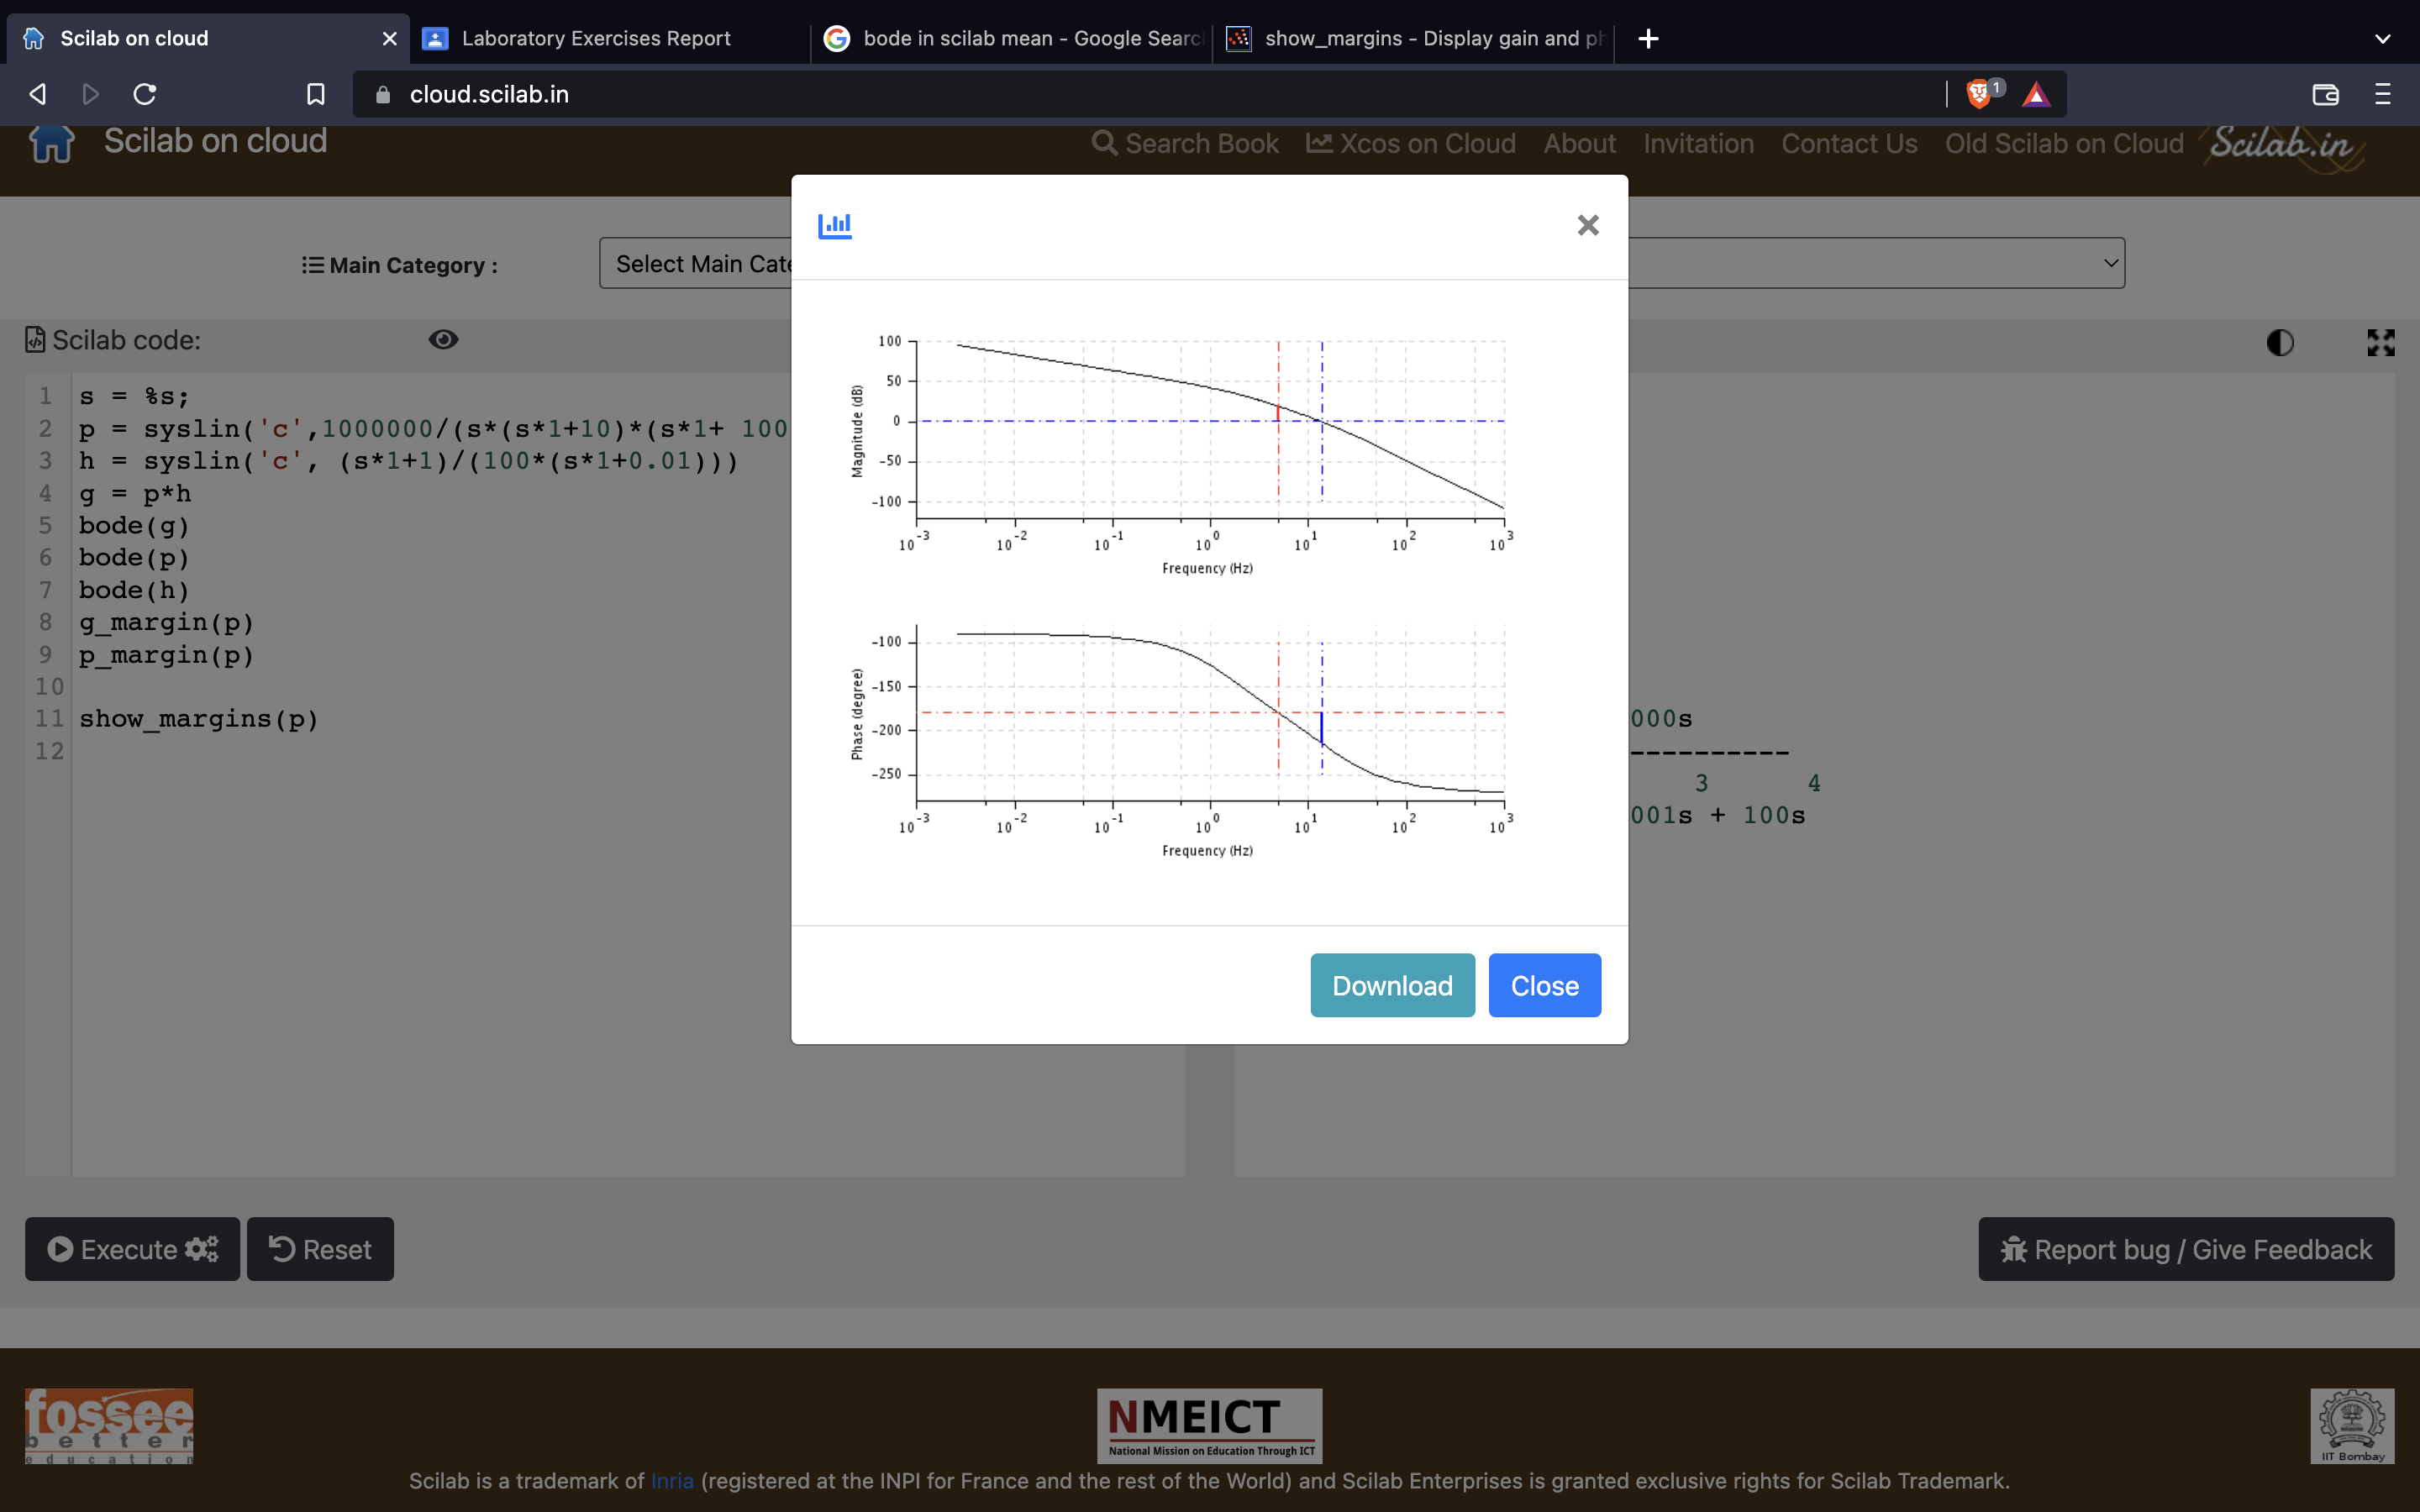
\includegraphics[width =20cm, height = 10cm]{images/bode plot.png}
        \caption{Graph}
        \label{Graph}
\end{figure}
\begin{figure}[!hth]
        \centering
        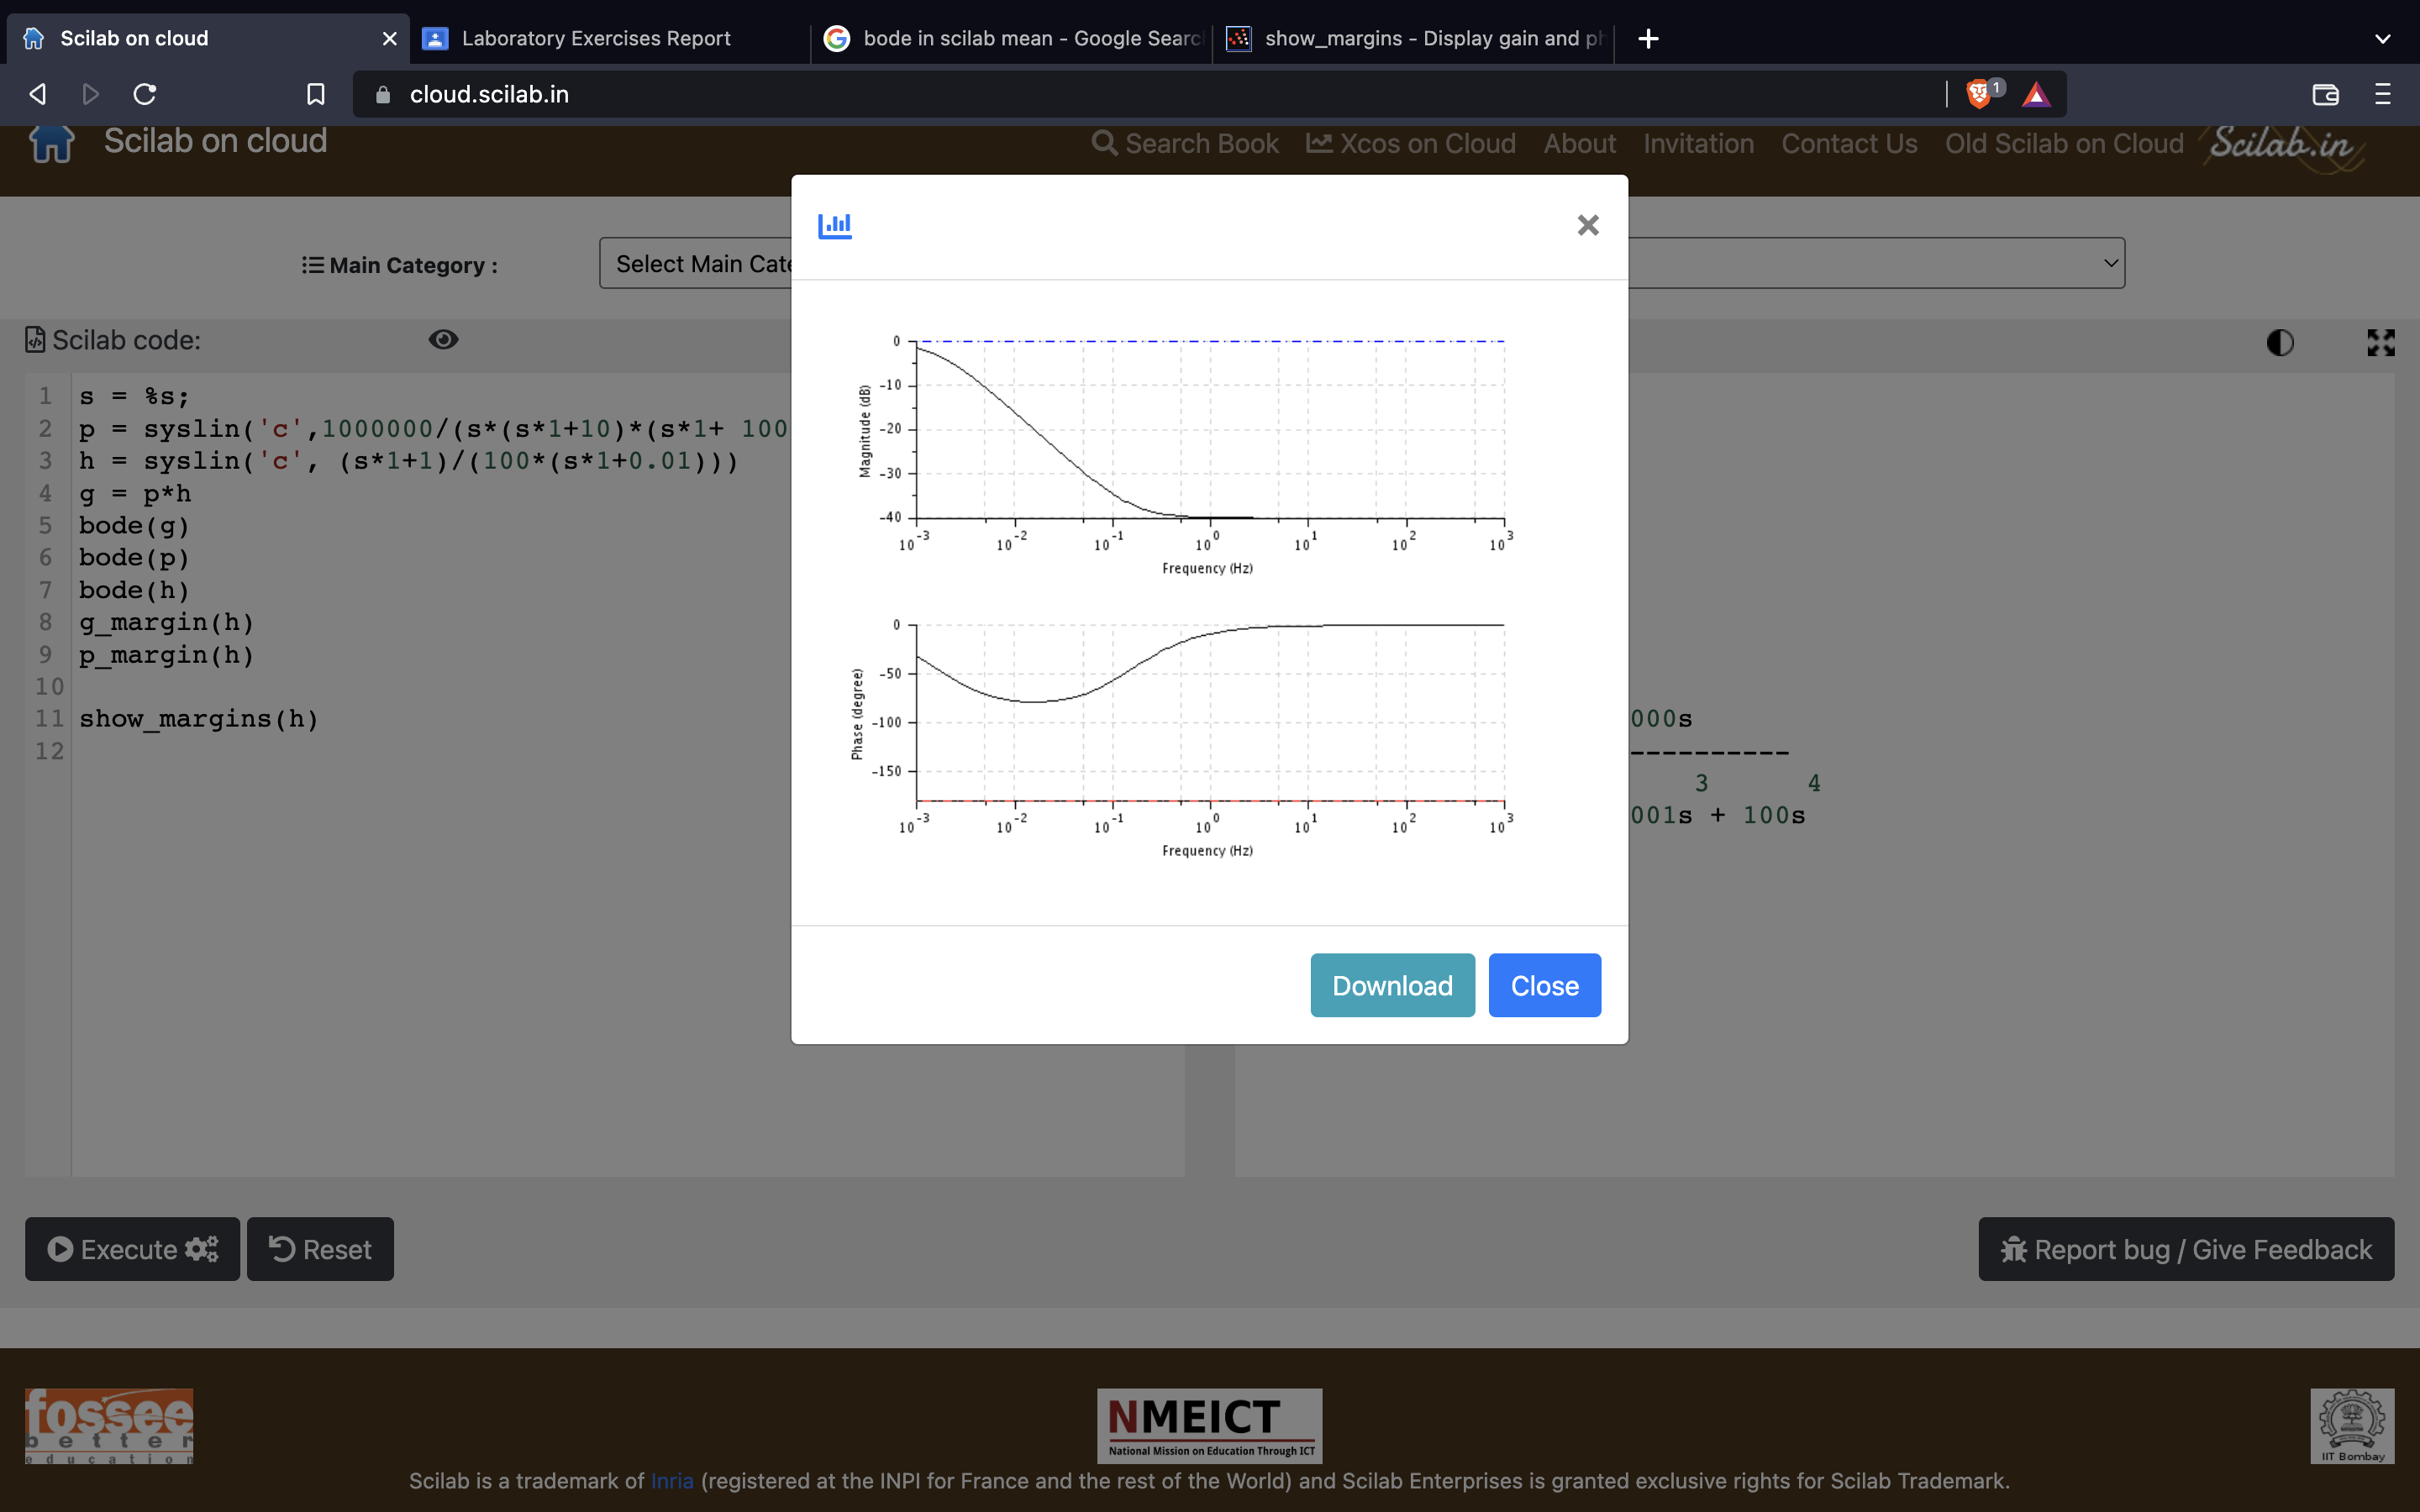
\includegraphics[width =20cm, height = 10cm]{images/bode ans.png}
        \caption{Graph}
        \label{Graph}
\end{figure}

\section*{\textcolor{black}{Observation and Conclusion}}
The stability of a system can be understood by the relation between gain and phase margin . If both GM and FM are positive system is stable , if both are equal to zero then marginally stable and if both are negative then unstable. 
In this case the FM and GM are both positive hence stable


\pagebreak

\begin{center}
    \LARGE {EXPT 17:Nyquist Plot}
             
\end{center}

\section*{\textcolor{black}{AIM: }}
\text{ To understand wheather a given open-loop system is stable when converted to closed-loop.}

\section*{\textcolor{black}{Block Diagram :}}

\begin{figure}[!hth]
        \centering
        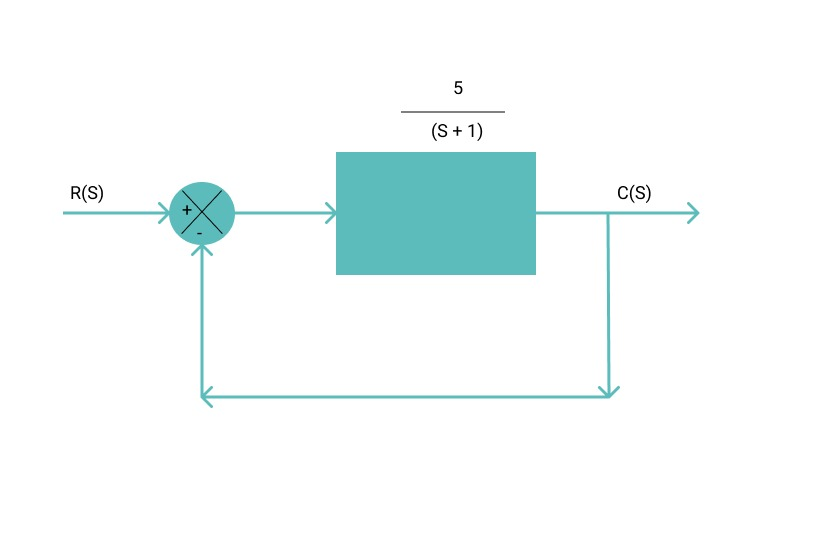
\includegraphics[width =20cm, height = 10cm]{images/Nyquist block..jpeg}
        \caption{Graph}
        \label{Graph}
\end{figure}

\section*{\textcolor{black}{Theory :}}
Nyquist plots, are commonly used in the frequency-response representation of linear, time-invariant, feedback control systems. Nyquist plots are polar plots, used for finding the stability of an open-loop system when converted to closed-loop system.
Here, z=n+p.
Where, no. of OLTF poles on RHS. no. of encirclements on .Positive for clockwise and negative for anti-clockwise, no. of CLTF zeroes on RHS.
For closed loop to be stable, z should be equal to zero, or n=-p .

 \par

\section*{\textcolor{black}{Code :}}

s = \%s;\\
g=5/(s-1);\\
G=syslin('c',g)\\
nyquist(G)\\


  \par 

\section*{\textcolor{black}{OUTPUT}}
We analyse the plots for 5 diff systems
1. g=5/(s-1)
2. g=120/(s-2)(s+6)(s+8)
3. g=50/(s-2)(s+6)(s+8)
4. g=(s+1)(s+2)/(s-3)(s-4)
5. g=10(s+1)(s+2)/(s-3)(s-4)

\begin{figure}[!hth]
        \centering
        \includegraphics[width =20cm, height = 10cm]{images/Nyquist Plot.png}
        \caption{Graph}
        \label{Graph}
\end{figure}
\begin{figure}[!hth]
        \centering
        \includegraphics[width =20cm, height = 10cm]{images/nyquist 2.png}
        \caption{Graph}
        \label{Graph}
\end{figure}
\begin{figure}[!hth]
        \centering
        \includegraphics[width =20cm, height = 10cm]{images/nyquist 3.png}
        \caption{Graph}
        \label{Graph}
\end{figure}
\begin{figure}[!hth]
        \centering
        \includegraphics[width =20cm, height = 10cm]{images/nyquist 4.png}
        \caption{Graph}
        \label{Graph}
\end{figure}
\begin{figure}[!hth]
        \centering
        \includegraphics[width =20cm, height = 10cm]{images/nyquist 5.png}
        \caption{Graph}
        \label{Graph}
\end{figure}

\section*{\textcolor{black}{Observation and Conclusion}}
To check the stability we check the number of encirclements around-1+jw and see the direction to get values of n and number of oltf poles on RHS of s-plane if n=-p then the system is stable.
So by that 1st, 2nd and 5th are stable systems.
So in this way we can check the stability of an open loop system when converted to closed loop, by the use of Nyquist Plot.
\pagebreak

\begin{center}
    \LARGE {EXPT 18:PID Control}
             
\end{center}

\section*{\textcolor{black}{AIM: }}
\text{ To understand the working of the speed control system of a motor using the properties of second order system.}

\section*{\textcolor{black}{Block Diagram :}}

\begin{figure}[!hth]
        \centering
        \includegraphics[width =20cm, height = 10cm]{images/pid block.jpeg}
        \caption{Graph}
        \label{Graph}
\end{figure}

\section*{\textcolor{black}{Theory :}}
The usefulness of PID controls lies in their general applicability to most control systems. In particular, when the mathematical model of the plant is not known and therefore analytical design methods cannot be used, PID controls prove to be most useful. If a mathematical model of the plant can be derived, then it is possible to apply various design techniques for determining parameters of the controller that will meet the transient and steady-state specifications of the closed-loop system. However, if the plant is so complicated that its mathematical model cannot be easily obtained, then an analytical or computational approach to the design of a PID controller is not possible. Then we must resort to experimental approaches to the tuning of PID controllers.

The transfer function of a PID controller is given as
kp + ki/s + kd*s

Here, kp acts as the stabilizer, ki acts as the integrator and kd acts as the differentiator.

 \par

\section*{\textcolor{black}{Code :}}

s = \%s;\\
col=['r','g','b','y','b']\\
for i=1:5\\
kp=10;\\
ki=8;\\
kd=i*2;\\
t=0:0.01:10;\\
G=syslin('c',1/((s+2)*(s+3)));\\
C=syslin('c',kp + ki/s + kd*s);\\
H=syslin('c',1/(s*0+1));\\
sys=(C*G)/.H;\\
plot(t, csim('step',t,sys),col(i));\\
end\\


  \par 

\section*{\textcolor{black}{OUTPUT}}

\begin{figure}[!hth]
        \centering
        \includegraphics[width =20cm, height = 10cm]{images/PID.png}
        \caption{Graph}
        \label{Graph}
\end{figure}

\section*{\textcolor{black}{Observation and Conclusion}}
The proportional integral derivative controller is used to improve the stability of the control system and to decrease steady state error.

\pagebreak
\end{document}
